

% ******************************* DIBRIS PhD Thesis Template **************************
% Please have a look at the README.md file for info on how to use the template

\documentclass[a4paper,12pt,oneside,times,authoryear,print,index]{Classes/PhDThesisPSnPDF}

% ******************************************************************************
% ******************************* Class Options ********************************
% *********************** See README for more details **************************
% ******************************************************************************

% `a4paper'(The University of Cambridge PhD thesis guidelines recommends a page
% size a4 - default option) or `a5paper': A5 Paper size is also allowed as per
% the Cambridge University Engineering Deparment guidelines for PhD thesis
%
% `11pt' or `12pt'(default): Font Size 10pt is NOT recommended by the University
% guidelines
%
% `oneside' or `twoside'(default): Printing double side (twoside) or single
% side.
%
% `print': Use `print' for print version with appropriate margins and page
% layout. Leaving the options field blank will activate Online version.
%
% `index': For index at the end of the thesis
%
% `draftclassic': For draft mode without loading any images (same as draft in book)
%
% `draft': Special draft mode with line numbers, images, and water mark with
% timestamp and custom text. Position of the text can also be modified.
%
% `abstract': To generate only the title page and abstract page with
% dissertation title and name, to submit to the Student Registry
%
% `chapter`: This option enables only the specified chapter and it's references
%  Useful for review and corrections.
%
% ************************* Custom Page Margins ********************************
%
% `custommargin`: Use `custommargin' in options to activate custom page margins,
% which can be defined in the preamble.tex. Custom margin will override
% print/online margin setup.
%
% *********************** Choosing the Fonts in Class Options ******************
%
% `times' : Times font with math support. (The Cambridge University guidelines
% recommend using times)
%
% `fourier': Utopia Font with Fourier Math font (Font has to be installed)
%            It's a free font.
%
% `customfont': Use `customfont' option in the document class and load the
% package in the preamble.tex
%
% default or leave empty: `Latin Modern' font will be loaded.
%
% ********************** Choosing the Bibliography style ***********************
%
% `authoryear': For author-year citation eg., Krishna (2013)
%
% `numbered': (Default Option) For numbered and sorted citation e.g., [1,5,2]
%
% `custombib': Define your own bibliography style in the `preamble.tex' file.
%              `\RequirePackage[square, sort, numbers, authoryear]{natbib}'.
%              This can be also used to load biblatex instead of natbib
%              (See Preamble)
%
% **************************** Choosing the Page Style *************************
%
% `default (leave empty)': For Page Numbers in Header (Left Even, Right Odd) and
% Chapter Name in Header (Right Even) and Section Name (Left Odd). Blank Footer.
%
% `PageStyleI': Chapter Name next & Page Number on Even Side (Left Even).
% Section Name & Page Number in Header on Odd Side (Right Odd). Footer is empty.
%
% `PageStyleII': Chapter Name on Even Side (Left Even) in Header. Section Number
% and Section Name in Header on Odd Side (Right Odd). Page numbering in footer

% Uncomment to change page style
%\pagestyle{PageStyleII}

% ********************************** Preamble **********************************
% Preamble: Contains packages and user-defined commands and settings
% ******************************************************************************
% ****************************** Custom Margin *********************************

% Add `custommargin' in the document class options to use this section
% Set {innerside margin / outerside margin / topmargin / bottom margin}  and
% other page dimensions
\ifsetCustomMargin
  \RequirePackage[left=37mm,right=30mm,top=35mm,bottom=30mm]{geometry}
  \setFancyHdr % To apply fancy header after geometry package is loaded
\fi


\usepackage{pdfpages}
%\usepackage{algorithmicx}


\usepackage{wrapfig}

\usepackage{amsmath}

\usepackage{tikz} %  for extensive game tree representation
\usetikzlibrary{positioning}
\usetikzlibrary{calc}
% to set line spaceing default is 'onehalf'
\usepackage{setspace}
%\doublespacing % or \doublespacing
\onehalfspacing % onehalf, default

% Add spaces between paragraphs
%\setlength{\parskip}{0.5em}
% Ragged bottom avoids extra whitespaces between paragraphs
\raggedbottom
% To remove the excess top spacing for enumeration, list and description
%\usepackage{enumitem}
%\setlist[enumerate,itemize,description]{topsep=0em}

%% track changes
%\usepackage[authormarkup=none]{changes} %% use this to see markup
\usepackage[final]{changes} %% use this to make final version without markup
\definechangesauthor[name={Per cusse}, color=orange]{MS} %% define  colors for different reviewers
\definechangesauthor[name={Per cusse}, color=blue]{EB}
\definechangesauthor[name={Per cusse}, color=green]{VS}
%% please check full documentation of 'changes' package


% *****************************************************************************
% ******************* Fonts (like different typewriter fonts etc.)*************

% Add `customfont' in the document class option to use this section

\ifsetCustomFont
  % Set your custom font here and use `customfont' in options. Leave empty to
  % load computer modern font (default LaTeX font).
  %\RequirePackage{helvet}

  % For use with XeLaTeX
  %  \setmainfont[
  %    Path              = ./libertine/opentype/,
  %    Extension         = .otf,
  %    UprightFont = LinLibertine_R,
  %    BoldFont = LinLibertine_RZ, % Linux Libertine O Regular Semibold
  %    ItalicFont = LinLibertine_RI,
  %    BoldItalicFont = LinLibertine_RZI, % Linux Libertine O Regular Semibold Italic
  %  ]
  %  {libertine}
  %  % load font from system font
  %  \newfontfamily\libertinesystemfont{Linux Libertine O}
\fi

% *****************************************************************************
% **************************** Custom Packages ********************************

% ************************* Algorithms and Pseudocode **************************


\usepackage{algorithm,algorithmicx}
\usepackage[noend]{algpseudocode}


% ********************Captions and Hyperreferencing / URL **********************

% Captions: This makes captions of figures use a boldfaced small font.
%\RequirePackage[small,bf]{caption}

\RequirePackage[labelsep=space,tableposition=top]{caption}
\renewcommand{\figurename}{Figure } %to support older versions of captions.sty

\usepackage{stackengine}

\usepackage{epigraph}
%\usepackage{subfig}
%\usepackage{subcaption}


% *************************** Graphics and figures *****************************

%\usepackage{rotating}
%\usepackage{wrapfig}

% Uncomment the following two lines to force Latex to place the figure.
% Use [H] when including graphics. Note 'H' instead of 'h'
%\usepackage{float}
%\restylefloat{figure}

% Subcaption package is also available in the sty folder you can use that by
% uncommenting the following line
% This is for people stuck with older versions of texlive
%\usepackage{sty/caption/subcaption}
\usepackage{subcaption}

%todo list
\usepackage{xcolor} 

\usepackage{todonotes}\setlength{\marginparwidth}{2.7cm}\reversemarginpar
%\reversemarginpar to have notes on the left margin (I have also modified the \marginparwidth otherwise the notes go out of the page)
% \todo{Comment}    % \todo[noline]{}   % \todo[inline]{}
% \todo[color=red!50]{Revision}
% \todo[color=blue!40]{Improve}
% \todo[color=purple!50]{Nice}

% ********************************** Tables ************************************
\usepackage{booktabs} % For professional looking tables
\usepackage{multirow}


%\usepackage{multicol}
%\usepackage{longtable}
%\usepackage{tabularx}


% *********************************** SI Units *********************************
\usepackage{siunitx} % use this package module for SI units


% ******************************* Line Spacing *********************************

% Choose linespacing as appropriate. Default is one-half line spacing as per the
% University guidelines

% \doublespacing
% \onehalfspacing
% \singlespacing


% ************************ Formatting / Footnote *******************************

% Don't break enumeration (etc.) across pages in an ugly manner (default 10000)
%\clubpenalty=500
%\widowpenalty=500

%\usepackage[perpage]{footmisc} %Range of footnote options

\newtheorem{proposition}{Proposition}
\newtheorem{definition}{Definition}
\newtheorem{theorem}{Theorem}
\newtheorem{proof}{Proof}


% *****************************************************************************
% *************************** Bibliography  and References ********************

%\usepackage{cleveref} %Referencing without need to explicitly state fig /table

% Add `custombib' in the document class option to use this section
\ifuseCustomBib
   \RequirePackage[square, sort, numbers, authoryear]{natbib} % CustomBib

% If you would like to use biblatex for your reference management, as opposed to the default `natbibpackage` pass the option `custombib` in the document class. Comment out the previous line to make sure you don't load the natbib package. Uncomment the following lines and specify the location of references.bib file

%\RequirePackage[backend=biber, style=numeric-comp, citestyle=numeric, sorting=nty, natbib=true]{biblatex}
%\bibliography{References/references} %Location of references.bib only for biblatex

\fi

% changes the default name `Bibliography` -> `References'
\renewcommand{\bibname}{References}
\usepackage{hyperref}
%\usepackage[colorlinks]{hyperref}
%
% \hypersetup{
%    citecolor=Violet,
%    linkcolor=Red,   
%    urlcolor=Magenta}


% ******************************************************************************
% ************************* User Defined Commands ******************************
% ******************************************************************************

% *********** To change the name of Table of Contents / LOF and LOT ************

%\renewcommand{\contentsname}{My Table of Contents}
%\renewcommand{\listfigurename}{My List of Figures}
%\renewcommand{\listtablename}{My List of Tables}


% ********************** TOC depth and numbering depth *************************

\setcounter{secnumdepth}{2}
\setcounter{tocdepth}{2}


% ******************************* Nomenclature *********************************

% To change the name of the Nomenclature section, uncomment the following line

%\renewcommand{\nomname}{Symbols}


% ********************************* Appendix ***********************************

% The default value of both \appendixtocname and \appendixpagename is `Appendices'. These names can all be changed via:

%\renewcommand{\appendixtocname}{List of appendices}
%\renewcommand{\appendixname}{Appndx}

% *********************** Configure Draft Mode **********************************

% Uncomment to disable figures in `draft'
%\setkeys{Gin}{draft=true}  % set draft to false to enable figures in `draft'

% These options are active only during the draft mode
% Default text is "Draft"
%\SetDraftText{DRAFT}

% Default Watermark location is top. Location (top/bottom)
%\SetDraftWMPosition{bottom}

% Draft Version - default is v1.0
%\SetDraftVersion{v1.1}

% Draft Text grayscale value (should be between 0-black and 1-white)
% Default value is 0.75
%\SetDraftGrayScale{0.8}


% ******************************** Todo Notes **********************************
%% Uncomment the following lines to have todonotes.

%\ifsetDraft
%	\usepackage[colorinlistoftodos]{todonotes}
%	\newcommand{\mynote}[1]{\todo[author=kks32,size=\small,inline,color=green!40]{#1}}
%\else
%	\newcommand{\mynote}[1]{}
%	\newcommand{\listoftodos}{}
%\fi

% Example todo: \mynote{Hey! I have a note}



% ************************ Thesis Information & Meta-data **********************
% Thesis title and author information, refernce file for biblatex
% ************************ Thesis Information & Meta-data **********************
%% The title of the thesis
\title{{Experimenting with Constraint Programming Techniques in 
		Artificial Intelligence: Automated System Design and 
		Verification of Neural Networks}}
%\texorpdfstring is used for PDF metadata. Usage:
%\texorpdfstring{LaTeX_Version}{PDF Version (non-latex)} eg.,
%\texorpdfstring{$sigma$}{sigma}

%% Subtitle (Optional)
%\subtitle{Using the Latex thesis template}

%% The full name of the author
\author{Andrea Gimellii}

%% Department (eg. Department of Engineering, Maths, Physics)
\dept{DIBRIS}

%% University and Crest
\university{University of Genova}

%% Full title of the Degree
\degreetitle{Master Degree}

\subject{LaTeX} \keywords{{LaTeX} {Master Thesis} {Computer Engineering } {University of
Genova}}

\DeclareMathOperator*{\argmax}{arg\,max}

%%%% CUSTOM COMMANDS %%%%
\newcommand{\liftcreate}{\textsc{LiftCreate}}
\newcommand{\liftcreatebf}{\textsc{LiftCreate-BF}}
\newcommand{\liftcreaters}{\textsc{LiftCreate-RS}}
\newcommand{\liftcreatehr}{\textsc{LiftCreate-HR}}
\newcommand{\liftcreatega}{\textsc{LiftCreate-GA}}
\newcommand{\liftcreatesmt}{\textsc{LiftCreate-SMT}}
\newcommand{\liftcreatecp}{\textsc{LiftCreate-CP}}
\newcommand{\never}{\textsc{NeVer}}
\newcommand{\nevertwo}{\textsc{NeVer2}}
\newcommand{\pynever}{\textsc{pyNeVer}}
\newcommand{\coconet}{\textsc{CoCoNet}}
\newcommand{\shark}{\textsc{shark}}
\newcommand{\hysat}{\textsc{HySAT}}
\newcommand{\pytorch}{\textsc{PyTorch}}
\newcommand{\tensorflow}{\textsc{TensorFlow}}
\newcommand{\gym}{\textsc{Gym}}
\newcommand{\stableb}{\textsc{Stable Baseline3}}
\newcommand{\pybullet}{\textsc{PyBullet}}
\newcommand{\drones}{\textsc{gym-pybullet-drones}}

\newcommand{\conc}[1]{\textsf{#1}}
\newcommand{\absc}[1]{\textsf{\textit{#1}}}


% ***************************** Abstract Separate ******************************
% To printout only the titlepage and the abstract with the PhD title and the
% author name for submission to the Student Registry, use the `abstract' option in
% the document class.

\ifdefineAbstract
 \pagestyle{empty}
 \includeonly{Declaration/declaration, Abstract/abstract}
\fi

% ***************************** Chapter Mode ***********************************
% The chapter mode allows user to only print particular chapters with references
% Title, Contents, Frontmatter are disabled by default
% Useful option to review a particular chapter or to send it to supervisior.
% To use choose `chapter' option in the document class

\ifdefineChapter
 \includeonly{Chapter3/chapter3}
\fi

% ******************************** Front Matter ********************************
\begin{document}

%%%%%%%%%%%%%%%%%%%%%%%%%%%%%%%%%%%%%%%%%%%%%%%%%%%%%%%%%%%%%%%%%%%%%%%%
%						TITLE PAGE							
%%%%%%%%%%%%%%%%%%%%%%%%%%%%%%%%%%%%%%%%%%%%%%%%%%%%%%%%%%%%%%%%%%%%%%%%
%% Also check thesis-info.tex page%%%%%

\thispagestyle{empty}
\begin{figure}[h!]
 \centering
 
\includegraphics[scale=0.20]{Logo_Unige.png} % here you can also place other logs, by properly adjusting the scale and margin
	\begin{center} 
		\Large
		%\textbf{\textsc{University of Genoa}}\\
		{\textsc{University of Genova}}\\
		  \vspace{0.5em}
		  \large
	         \textsc{Master thesis in Computer Engineering}\\

	\end{center}
\end{figure}



\begin{center} 
	
	%\vspace{1em}


		\Large
		\textbf{Verification of neural networks} \\
\end{center}

 	\begin{center} 
		by \\
		\vspace{0.5em}
		\textbf{Andrea Gimelli}\\
		\vspace{1em}
	
		
	%\textsc{Doctoral School in Sciences and Technologies for Information and Knowledge} \\
    \vspace{0.5em}
	\vspace{1cm}	
		\normalsize
		Thesis submitted for the degree of \textit{Master degree} ($35^\circ$ cycle) \\
	\vspace{1cm}	
		\normalsize
		May 2023\\ 
	\end{center}
	\vspace{2em}

\vfill


	\noindent {Armando Tacchella} \hfill  {Supervisor}	
	\\
	\noindent {Stefano Demarchi}  \hfill  {Relator}	


\vspace{2em}
\vfill
\begin{figure}[h!]
 \centering
 
\includegraphics{Logo_Dibris.png}
\begin{center} 
		\small{Department of Informatics, Bioengineering, Robotics and Systems Engineering\\}
	\end{center}
\end{figure}
	

%%%%%%%%%%%%%%%%%%%%%%%%%%%%%%%%%%%%%%%%%%%%%%%%%%%%%%%%%%%%%%%%%%%%%%%%



\frontmatter

%\maketitle

%% ******************************* Thesis Dedidcation ********************************

\begin{dedication} 

I would like to dedicate this thesis to  \dots

\end{dedication}


%% ******************************* Thesis Declaration ***************************

\begin{declaration}

I hereby declare that except where specific reference is made to the work of 
others, the contents of this dissertation are original and have not been 
submitted in whole or in part for consideration for any other degree or 
qualification in this, or any other university. This dissertation is my own 
work and contains nothing which is the outcome of work done in collaboration 
with others, except as specified in the text and Acknowledgements. This 
dissertation contains fewer than 65,000 words including appendices, 
bibliography, footnotes, tables and equations and has fewer than 150 figures.

% Author and date will be inserted automatically from thesis.tex \author \degreedate

\end{declaration}


% ************************** Thesis Acknowledgements **************************

\begin{acknowledgements}      

    To all who helped the University of Genoa complete my master's thesis, I would like to take this opportunity to express my sincere gratitude.
    First and foremost, I want to express my gratitude to Prof. Armando Tacchella for his invaluable advice, steadfast support, and ongoing encouragement throughout this research process. He played a key role in the development of this thesis and my academic development with his knowledge, commitment, and patience. 
    Additionally, I would like to express my sincere gratitude to Stefano Demarchi, who served as my thesis advisor. His advice and expertise were very helpful in helping me to improve the methodology and content of my research. 
    I owe a debt of gratitude to Genoa University's faculty and staff for creating a welcoming learning environment and providing necessary tools for my research. My learning experience has been greatly enhanced by their dedication to excellence. 
    I want to thank my classmates and coworkers for their help and cooperation. They contributed thoughtful ideas, shared their expertise, and took part in insightful discussions. In helping me to develop my ideas and widen my perspective, their contributions have been invaluable. 
    I'm appreciative of my friends' and family's unwavering support, inspiration, and tolerance throughout this difficult academic endeavor. They have been a constant source of inspiration because they believe in me and are present. 
    Finally, I would like to express my sincere gratitude to all the people, groups, and institutions who have kindly helped my research by contributing information, materials, or any other kind of support. This thesis would not have been successful without your assistance. 
    Please know that your contributions have not gone unnoticed and are greatly valued even though it is impossible to specifically thank each individual. 
    I'd like to thank everyone for their encouragement, support, and belief in my abilities. I sincerely appreciate your invaluable contributions to my master's thesis at the University of Genoa, and I do so with the utmost honor and gratitude. 
    percent. 
\end{acknowledgements}

% ************************** Thesis Abstract *****************************
% Use `abstract' as an option in the document class to print only the titlepage and the abstract.
\begin{abstract}
	% Context
	This thesis focuses on the application of Constraint Satisfaction and Optimization
	techniques in two Artificial Intelligence (AI) domains: automated design of elevator
	systems and verification of Neural Networks (NNs). The three main areas of interest
	for my work are $(i)$ the languages for defining the constraints for the systems, 
	$(ii)$ the algorithms and encodings that enable solving the problems considered and
	$(iii)$ the tools that implement such algorithms. 
	
	% Motivation
	Given the expressivity of the domain description languages and the availability of
	effective tools, several problems in diverse application fields have been solved 
	successfully using constraint satisfaction techniques. The two case studies herewith
	presented are no exception, even if they entail different challenges in the adoption
	of such techniques. Automated design of elevator systems not only requires encoding
	of feasibility (hard) constraints, but should also take into account design preferences, 
	which can be expressed in terms of cost functions whose optimal or near-optimal value
	characterizes ``good'' design choices versus ``poor'' ones.  Verification of NNs (and
	other machine-learned implements) requires solving large-scale constraint problems
	which may become the main bottlenecks in the overall verification procedure. 
	
	% Contribution
	This thesis proposes some ideas for tackling such challenges, including encoding 
	techniques for automated design problems and new algorithms for handling the optimization
	problems arising from verification of NNs. The proposed algorithms and techniques are
	evaluated experimentally by developing tools that are made available to the research
	community for further evaluation and improvement.
\end{abstract}


% *********************** Adding TOC and List of Figures ***********************
%\newpage
%\listofchanges % this will be useful while revision, to see all markups (see preamble, comment line 35 and uncomment line 34)..

%\tableofcontents

%\listoffigures

%\listoftables

% \printnomenclature[space] space can be set as 2em between symbol and description
%\printnomenclature[3em]

\printnomenclature

% ******************************** Main Matter *********************************
\mainmatter

%*******************************************************************************
%******************************** Introduction *********************************
%*******************************************************************************
\chapter{Introduction}

\section{Context and motivation}
\label{sec:context}

\subsection{Neural networks verification}

Adoption and successful application of deep neural networks (DNNs) in various 
domains have made them one of the most popular machine-learned models to date 
--- see, e.g.,~\cite{DBLP:conf/cvpr/TaigmanYRW14} on image 
classification,~\cite{DBLP:journals/taslp/YuHMCS12} on speech recognition,
and~\cite{DBLP:journals/nature/LeCunBH15} for the general principles and a 
catalog of success stories. Despite the impressive progress that the learning 
community has made with the adoption of DNNs, it is well known that their 
application in safety- or security-sensitive contexts is not yet hassle-free. 
From their well-known sensitivity to \textit{adversarial perturbations}
\cite{DBLP:journals/corr/GoodfellowSS14,DBLP:journals/corr/SzegedyZSBEGF13}, 
i.e., minimal changes to correctly classified input data that cause a network 
to respond in unexpected and incorrect ways, to other less-investigated, but 
possibly significant properties --- see, 
e.g.,~\cite{DBLP:journals/corr/abs-1805-09938} for a catalog 
--- the need for tools to analyze and possibly repair DNNs is strong.

As witnessed by an extensive survey~\cite{huang2018safety}
of more than 200 recent papers, the response from the scientific
community has been equally strong. 
As a result, many algorithms have been proposed for the verification 
of neural networks and tools implementing them have been made
available. Some examples of well-known and fairly mature verification
tools are Marabou~\cite{DBLP:conf/cav/KatzHIJLLSTWZDK19}, a
satisfiability modulo theories (SMT)-based tool that answers queries
regarding the properties of a DNN by transforming the queries into 
constraint satisfiability problems; ERAN~\cite{DBLP:conf/iclr/SinghGPV19}, 
a robustness analyzer based on abstract interpretation and 
MIPVerify~\cite{DBLP:conf/iclr/TjengXT19},
another robustness analyzer based on mixed integer programming
(MIP). Other widely-known verification tools are
Neurify~\cite{DBLP:conf/nips/WangPWYJ18}, a robustness analyzer based
on symbolic interval analysis and linear relaxation,
NNV~\cite{DBLP:journals/corr/abs-2004-05519}, a tool implementing
different methods for reachability analysis,
Sherlock~\cite{DBLP:conf/hybrid/DuttaCJST19}, an output range analysis
tool and NSVerify~\cite{DBLP:conf/kr/AkitundeLMP18}, also for
reachability analysis. A number of verification methodologies ---
without a corresponding tool --- is also available
like~\cite{DBLP:journals/corr/abs-1807-03571}, a game-based 
methodology for evaluating pointwise robustness of neural networks in
safety-critical applications. Most of the above-mentioned tools and
methodologies work only for feedforward fully-connected neural
networks with ReLU activation functions, with some of them
featuring verification algorithms for convolutional neural networks 
with different kinds of activation function. To the best of our
knowledge, current state-of-the-art tools are restricted to
verification/analysis tasks, in some cases they are limited to
specific network architectures and they might prove difficult to use
for practitioners and, in general, those who are not familiar with
the complete background.

Our tool \nevertwo{} finds itself at the intersection of the
issues explained above, and aims to bridge the gap between
learning and verification of DNNs. \nevertwo{} borrows its design
philosophy from \never{}~\cite{pulina2011n}, the first tool for 
automated learning, analysis and repair of neural networks. 
\never{} was designed to deal with multilayer perceptrons 
(MLPs) and its core  was an abstraction-refinement mechanism 
described in~\cite{DBLP:conf/cav/PulinaT10,DBLP:journals/aicom/PulinaT12}.  
As a system, one peculiar aspect of \never{} was that it included
learning capabilities through the \shark~\cite{igel08} library.
Concerning the verification part, \never{} could utilize any
solver integrating Boolean reasoning and linear arithmetic constraint
solving --- \hysat~\cite{franzle2007efficient} at the time.
A further peculiarity of the approach was that \never{}
could leverage abstract counterexamples to (try to) repair the
MLP, i.e., retrain it to eliminate the causes of misbehaviour.
\nevertwo{} relies on the \pynever{} API~\cite{guidotti2021pynever}
and a first description of the system is available 
in~\cite{guidotti2020never}, where the verification capabilities
were provided by external tools like Marabou, ERAN and MIPVerify.
This Thesis describes the new abstraction-refinement procedure
implemented by \nevertwo{} and formalizes all the theorems involved.
The version of \nevertwo{} corresponding to this work is available 
online~\cite{never2online} under the Commons Clause (GNU GPL v3.0) 
license.

\clearpage


%\section{Contribution}
\label{sec:contribution}

The contribution of this Thesis is twofold. First, the results of the
experiments on different ways of encoding design problems and how to
employ constraint satisfaction techniques in verification of NNs contribute
to deepen the knowledge in how different ways of encoding the constraints
impact on the results. Second, for both case studies we developed special
purpose tools that provide access to all the methodologies taken in exam.
In particular, we contribute with the following results:

\paragraph{Declarative encodings for elevator systems.}
Starting from the work presented in~\cite{AiLift2} we investigated how to
benefit from declarative encodings in the elevator domain, and how to
transfer such knowledge to generic configuration systems. In~\cite{AiLift3}
and~\cite{AiLift4} we experimented with several declarative encodings based
on Genetic Algorithms (GAs), Satisfiability Modulo Theories (SMT) and 
Constraint Programming (CP) showing the strength and weaknesses of these
approaches against the different aspects of the design task.

\paragraph{Neural networks verification in safety-critical domains.}
We use SMT as a pivot to deal with the verification of machine learning 
models with neural networks. We created a standard for the definition
of benchmarks which uses SMT as the language for the definition of the
verification properties~\cite{vnnlib} and we contribute with two new case
studies, i.e., Adaptive Cruise Control (ACC)~\cite{DBLP:conf/ecms/DemarchiGPT22}
and drone hovering. We also experiment with optimization algorithms for
our verification procedure~\cite{DBLP:conf/cpsschool/DemarchiG22}.

\paragraph{State of the art tool development.}
Alongside the encodings and the experiments herewith reported, we also
developed new tools for providing fast and easy access to the algorithms.
For the design of elevator systems we perfectioned the tool \liftcreate,
which provides an interface towards the different encodings. Using this
tool, the experiments shared the same overhead and provided reliable and
replicable results.

In the verification topic, we created a software portfolio named
\textit{NeVerTools}\footnote{https://github.com/NeVerTools} which groups
the former contributions in the domain, packed in the \pynever{} Python API
and two Graphical User Interfaces (GUIs), namely \coconet{} and \nevertwo.
%\section{Overview}
\label{sec:overview}

The manuscript is structured as follows. Chapter~\ref{ch:background} resumes the
relevant background notions for elevator systems, neural networks and the main
techniques employed. In the first part, Chapter~\ref{ch:elevator_model} details
the modeling of elevator systems with variables, constraints and objectives and
Chapter~\ref{ch:elevator_enc} enumerates the different encodings that we propose
for replacing the current engine. After showcasing the web application for 
elevator design in Chapter~\ref{ch:liftcreate}, in Chapter~\ref{ch:experiments_design}
we show our experimental campaign for the search of a new declarative encoding.

In the second part we focus on neural networks, and we meticulously detail the
abstraction algorithms in Chapter~\ref{ch:abstraction}. Then we detail the tools
we developed in order to foster research and collaboration in Chapter~\ref{ch:never2}
and we collect the results of this topic in Chapter~\ref{ch:experiments_nn}.
Finally, Chapter~\ref{ch:conclusions} concludes the Thesis and sheds some light on
possible future research perspectives.

\chapter{Background}
\label{ch:background}
%\section{A primer on elevator systems}
\label{sec:elevators}

Elevator systems are characterized by different lifting mechanisms, 
e.g., hydraulic cylinders or electric motors, and different setups,
e.g., one or two cylinders, presence or absence of counterweights, and
dedicated machine room versus machine-room-less implements. In this
paper, we focus on Roped Hydraulic Elevators (RHEs), in which the
lifting power is provided by hydraulics. In Fig.~\ref{img:planView}
we show the cross-section of a RHE similar to those produced by
\liftcreate{}. Note that the image has been modified by removing 
some parts while enhancing others to ease understanding by a 
non-technical audience. The plan view accounts for the main components 
to be found in the design of an elevator. In the figure, the 
\textit{shaft} denotes the enclosure space in which the elevator 
is installed. Inside the shaft, we can observe the \textit{hydraulic
	cylinder}, providing lifting power, and  the \textit{car} attached
to the \textit{car frame}, a mechanical structure that supports the 
car and connects it to the piston through \emph{ropes} (not visible
in the plan view).  
The car frame slides within the shaft along the \textit{car rails}. 
The ropes are guided through a \textit{pulley} attached on top of the
piston: one end is secured to the shaft base, the other to the car frame.
Finally there are two kinds of doors, namely the \textit{car door} and
the  \textit{landing door}. As the name implies, the car door is only
one and it is attached to the car, while there is one matching landing
door for each floor.

\begin{figure}[t!]
	\caption{\label{img:planView} Cross-section (plan view) of a
		configured RHE. The shaft is the gray box surrounding the
		other components, the car frame is on the left side and
		doors at the bottom of the drawing.}
	\centering 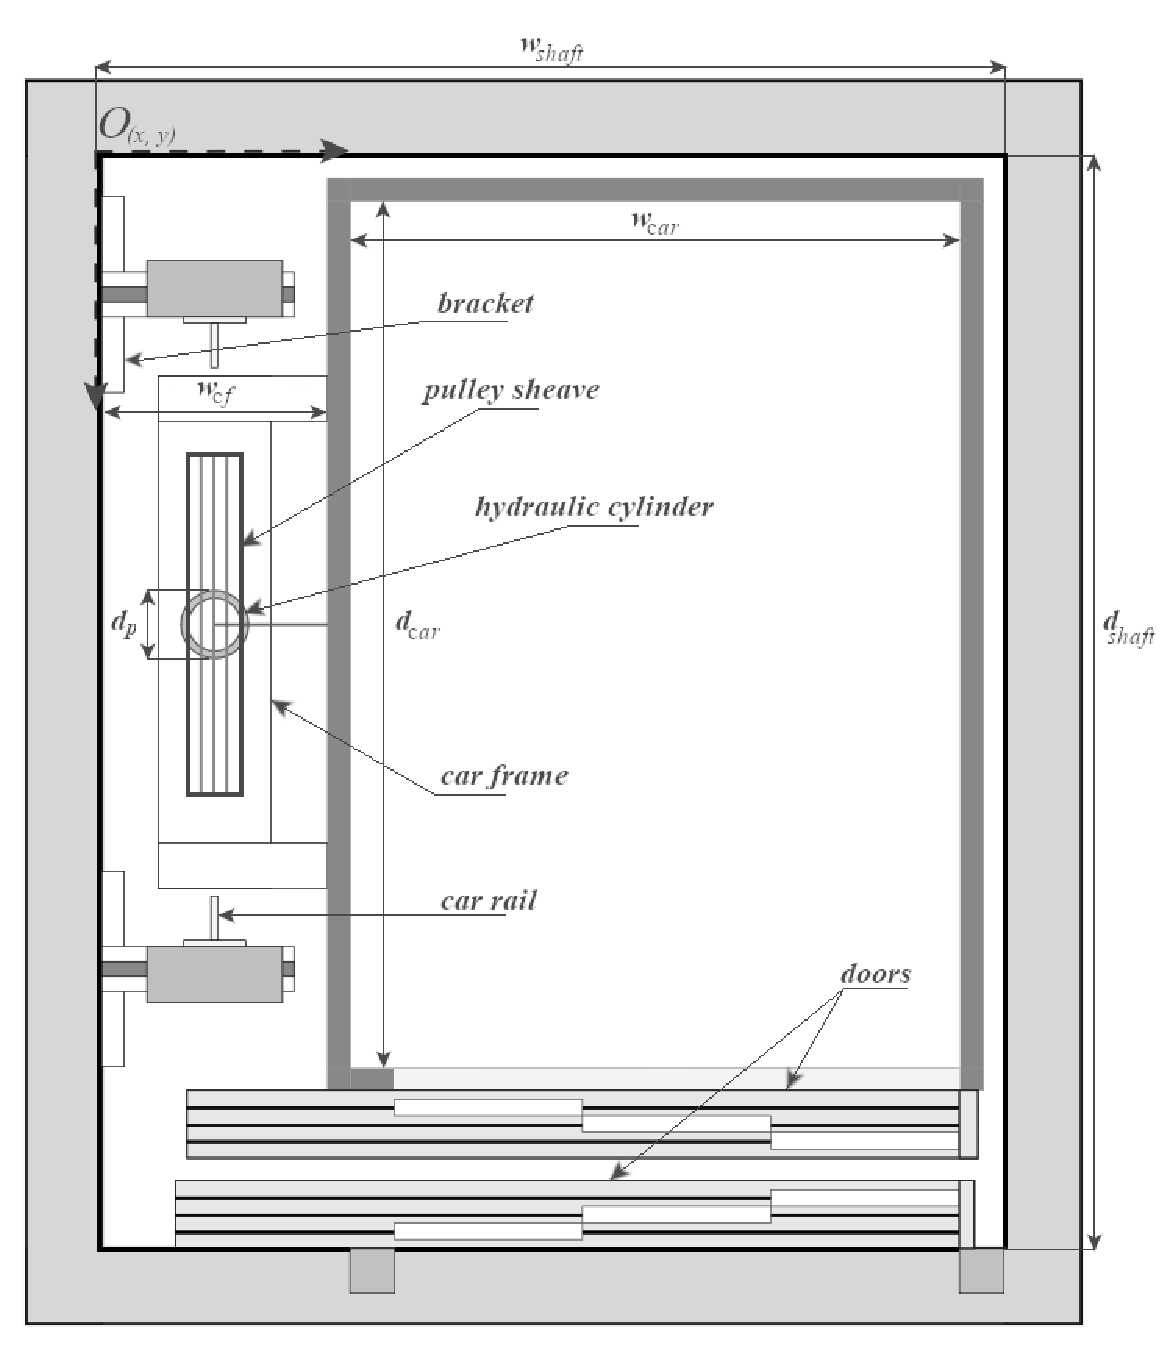
\includegraphics[width=.9\linewidth]{Elevator/planView.eps}
\end{figure}

Design of RHEs is usually performed in steps. The first one is the
choice of the doors and the car frame, whose positioning must be
determined considering shaft size, encumbrances, and tolerances since
a minimum distance between moving and fixed parts must always be taken
into account. In the second step, considering other parameters
like the distance between the car and the shaft or the materials used
for the car, an overall suspended weight and a maximum payload can
be computed. Based on these findings, other components like ropes,
rails, safety gear and the hydraulic cylinder can be engineered,
making sure that compliance to the norms and regulations is always
respected. In this phase, review of the previous phases might be
necessary because some choices might not result in feasible solutions,
which often makes the (manual) process to obtain the final design an
iterative trial-and-error endeavor. 
Considering the plan view of the of RHEs in Fig.\ref{img:planView}, 
in this work we  focus on elevators whose car frame is installed on the
left side and doors are installed at the bottom of the drawing. The
component selection we consider is limited to car frame, doors and
hydraulic cylinder, whereas placement involves car frame and doors.
\section{Neural Networks}
\label{sec:nns}

\paragraph{Basic notation and definitions.} 
We denote $n$-dimensional \emph{vectors} of real numbers 
$x \in \mathbb{R}^n$ --- also \emph{points} or \emph{samples} 
--- with lowercase letters like $x, y, z$. We write
$x = (x_1, x_2, \ldots, x_n)$ to denote a vector with
its \emph{components} along the $n$ coordinates. We denote $x \cdot y$
the \emph{scalar product} of two vectors $x, y \in \mathbb{R}^n$
defined as $x \cdot y = \sum_{i=1}^n x_i y_i$. The \emph{norm} $\lVert
x \rVert$ of a vector is defined as $\lVert x \rVert = \sqrt{x \cdot x}$.
We denote sets of vectors $X \subseteq \mathbb{R}^n$ with uppercase
letters like $X, Y, Z$.  A set of vectors $X$ is  
\emph{bounded} if there exists $r \in \mathbb{R}, r > 0$ such that 
$\forall x, y \in X$ we have $d(x, y) < r$ where $d$ is the 
\emph{Euclidean norm} $d(x, y) = \lVert x - y \rVert$. 
A set $X$ is \emph{open} if for every point $x \in X$ there 
exists a positive real number $\epsilon_x$ such that a point
$y \in \mathbb{R}^n$ belongs to $X$ as long as $d(x,y)
< \epsilon_x$. The complement of an open set is a \emph{closed} set ---
intuitively, one that includes its boundary, whereas open sets do not;
closed and bounded sets are \emph{compact}. A set $X$ is \emph{convex}
if for any two points $x,y \in X$ we have that also $z \in X~\forall 
z = (1 - \lambda)x + \lambda y$ with $\lambda \in
[0,1]$, i.e., all the points falling on the
line passing through $x$ and $y$ are also in $X$. Notice that the
intersection of any family, either finite or infinite, of convex sets
is convex, whereas the union, in general, is not. Given any
non-empty set $X$, the smallest convex set $\mathcal{C}(X)$
containing $X$ is the \emph{convex hull of} $X$ and it is
defined as the intersection of all convex sets containing
$X$. A \emph{hyperplane} $H \subseteq \mathbb{R}^n$ can be
defined as the set of points
\begin{equation*}
	H = \{x \in \mathbb{R}^n \mid a_1x_1 + a_2x_2 + \ldots + a_n x_n =
	b\}
\end{equation*}
where $a \in \mathbb{R}^n$, $b \in \mathbb{R}$ and at least one
component of $a$ is non-zero. Let $f(x) = a_1x_1 + a_2x_2 + \ldots +
a_n x_n - b$ be the affine form defining $H$. The \emph{closed half-spaces
	associated with} $H$ are defined as
\begin{equation*}
	H_{+}(f) = \{x \in X \mid f(x) \geq 0 \} \qquad  H_{-}(f) = \{x \in
	X \mid f(x) \leq 0 \}
\end{equation*}
Notice that both $H_{+}(f)$ and $H_{-}(f)$ are convex. A
\emph{polyhedron} in $P \subseteq \mathbb{R}^n$ is a set of points 
defined as $P= \bigcap_{i=1}^p C_i$ where $p \in \mathbb{N}$ is a
finite number of closed half-spaces $C_i$. A bounded polyhedron is a
\emph{polytope}: from the definition, it follows that polytopes are 
convex and compact in $\mathbb{R}^n$. 


\paragraph{Neural networks.} Given a finite number $p$ of functions 
$f_1: \mathbb{R}^n  \to \mathbb{R}^{n_1}, \ldots, f_p:
\mathbb{R}^{n_{p-1}} \to \mathbb{R}^{m}$ --- also called \emph{layers}
--- we define a \emph{feed forward neural network}~\cite{abdi1999neural}
as a function $\nu : \mathbb{R}^n \to \mathbb{R}^m$ obtained through
the compositions of the layers, i.e.,  $\nu(x) = f_p(f_{p-1}( \ldots
f_1(x) \ldots ))$. The layer $f_1$ is called \emph{input layer}, the
layer $f_p$ is called \emph{output layer}, and  the remaining layers
are called \emph{hidden}. For $x \in \mathbb{R}^n$, we consider only
two types of layers:
\begin{itemize}
	\item $f(x) = Ax + b$ with $A \in \mathbb{R}^{m \times n }$ and $b
	\in \mathbb{R}^m$ is an \emph{affine layer} implementing the
	linear mapping $f : \mathbb{R}^n \to 
	\mathbb{R}^m$;
	\item $f(x) = (\sigma_1(x_1), \ldots, \sigma_n(x_n))$ is a
	\emph{functional layer} $f: \mathbb{R}^n \to \mathbb{R}^n$
	consisting of $n$ \emph{activation 
		functions} --- also called \emph{neurons}; usually
	$\sigma_i = \sigma$ 
	for all $i \in [1,n]$, i.e., the function $\sigma$ is applied
	componentwise to the vector $x$. 
\end{itemize}
We consider two kinds of activation functions $\sigma: \mathbb{R} \to
\mathbb{R}$ that find widespread adoption: the \emph{ReLU} function
defined as $\sigma(r) = max(0,r)$, and the \emph{logistic} function
defined as $\sigma(r) = \frac{1}{1 + e^{-r}}$.
Although we do not consider them here, affine mappings
can also represent convolutional layers with one or more filters~\cite{DBLP:conf/sp/GehrMDTCV18}.
For a neural network $\nu : \mathbb{R}^n \to
\mathbb{R}^m$, the task of \emph{classification} is about assigning to
every input vector $x \in \mathbb{R}^n$ one out of $m$ labels: an
input $x$ is assigned to a class $k$ when $\nu(x)_k > \nu(x)_j$ for
all $j \in [1,m]$ and $j \neq k$; the task of \emph{regression} is
about approximating a functional mapping from $\mathbb{R}^n$ to
$\mathbb{R}^m$. 
In this regard, neural networks consisting of affine layers
coupled with either ReLUs or logistic layers offer universal
approximation capabilities~\cite{hornik1989multilayer}.

\paragraph{Verification task.} Given a neural network $\nu :
\mathbb{R}^n \to \mathbb{R}^m$ we wish to verify algorithmically that
it complies to stated \emph{post-conditions} on the output as long as
it satisfies \emph{pre-conditions} on the input. Without loss of
generality\footnote{Input domains must be bounded to enable
	implementation of neural networks on digital hardware; therefore,
	also data from physical processes, which are potentially ubounded,
	are normalized within small ranges in practical applications.},
we assume that the input domain of $\nu$ is a bounded set $I 
\subset \mathbb{R}^n$. Therefore, the corresponding output domain is 
also a bounded set $O \subset \mathbb{R}^m$ because $(i)$ affine
transformations of bounded sets are still bounded sets, $(ii)$ ReLU is a
piecewise affine transformation of its input, $(iii)$ the output
of logistic functions is always bounded in the set $[0,1]$, and the
composition of bounded functions is still bounded. We
require that the logic formulas defining pre- and post-conditions are
interpretable as finite unions of bounded sets in the input 
and output domains. Formally, given $p$ bounded sets $X_1, \ldots,
X_p$ in $I$ such that $\Pi = \bigcup_{i=1}^p X_i$ and $s$ bounded
sets $Y_1, \ldots, Y_s$ in $O$ such that $\Sigma =
\bigcup_{i=1}^s Y_i$, we wish to prove that  
\begin{equation}
	\label{eq:verif}
	\forall x \in \Pi. \nu(x) \in \Sigma.
\end{equation}
While this query cannot express some problems regarding
neural networks, e.g., invertibility or
equivalence~\cite{DBLP:journals/corr/abs-1805-09938}, it captures the
general problem of testing robustness against \emph{adversarial
	perturbations}~\cite{DBLP:journals/corr/GoodfellowSS14}. For example,
given a network $\nu : I \to O$ with $I \subset \mathbb{R}^n$ and
$O \subset \mathbb{R}^m$ performing a 
classification task, we have that separate regions of the input are 
assigned to one out of $m$ labels by $\nu$. Let us assume
that region $X_j \in I$ is classified in the $j$-th class
by $\nu$. We define an \emph{adversarial region} as a
set $\hat{X}_j$ such that for all $\hat{x} \in \hat{X}$ there exists at
least one $x \in X$ such that $d(x,\hat{x}) \leq \delta$ for some
positive constant $\delta$. The 
network $\nu$ is \emph{robust} with respect to $\hat{X}_j \subseteq I$ if,
for all $\hat{x} \in \hat{X}_j$, it is still the case that $\nu(x)_j > \nu(x)_i$
for all $i \in [1,m]$ with $i \neq j$. This can be stated in the
notation of condition (\ref{eq:verif}) by letting $\Pi = \{ \hat{X}_j 
\}$ and $\Sigma = \{ Y_j \}$ with $Y_j = \{ y \in O \mid y_j \geq y_i
+ \epsilon, \forall i \in [1,n] \wedge i \neq j, \epsilon >
0\}$. Analogously, in 
a regression task we may ask that points that are sufficently close to
any input vector in a set $X \subseteq I$ are also sufficiently close
to the corresponding output vectors. To do this, given the positive
constants $\delta$ and $\epsilon$, we let $\hat{X} = \{ \hat{x} \in I
\mid \exists x. (x \in X \wedge d(\hat{x},x) \leq  \delta) \}$ and $\hat{Y}
= \{\hat{y} \in O \mid \exists x. (x \in \hat{X} \wedge d(\hat{y},\nu(x)) \leq
\epsilon)\}$ to obtain  
$\Pi = \{\hat{X}\}$ and $\Sigma = \{\hat{Y}\}$. Notice that, given our
definition, we consider adversarial regions and output images 
that may not be convex.
%

%\section{Constraint Satisfaction Problems}

A Constraint Satisfaction Problem (CSP) requires a value, selected 
from a given finite domain, to be assigned to each variable in the 
problem, so that all constraints relating the variables are
satisfied~\cite{brailsford1999constraint}. In more detail, given a 
set of variables together with their domains, i.e., a set of possible 
values that can be assigned to each variable, and a description of 
the problem in the form of mathematical constraints, a CSP is the 
problem of finding values of the variables that satisfy every 
constraint. It is defined as a set of $n$ \textit{variables} 
$X = \{x_1, \ldots, x_n\}$, a set of current \textit{domains}
$\mathcal{D} = \{D(x_1), \ldots, D(x_n)\}$ where $D(x_i)$ is the
finite set of possible \textit{values} for variable $x_i$, and a 
set $\mathcal{C}$ of \textit{constraints} between variables.
A constraint $C$ on the set of variables $X(C) = (x_{i_1}, \ldots, 
x_{i_r})$ is a subset of the Cartesian product $D_0(x_{i_1}) \times 
\ldots \times D_0(x_{i_r})$ that specifies the \textit{allowed}
combinations of values for the variables $x_{i_1} \times \ldots
\times x_{i_r}$.
 
In this Thesis we consider two main approaches to solve CSPs, 
namely Constraint Programming (CP) and Satisfiability
Modulo Theory (SMT). CP is a powerful paradigm for solving CSPs
that draws on a wide range of techniques from artificial 
intelligence, operations research, algorithms, graph theory and 
others~\cite{rossi2006handbook}. In general, CP provides high level
languages that allow one to describe (model) a problem in a 
declarative way by means of constraints, that is, properties of the
solutions to be found. Product configuration has been established 
as a successful application area of CP~\cite{mcdonald2002case,
	jensen2004clab, benavides2005using, falkner2011modeling,
	hervieu2016practical}. A CP solver  checks whether a certain
assignment of decision variables respects all the constraints, 
and returns such assignment in that case. Most CP solvers deal 
naturally with finite domains and have good propagators to handle
injectivity constraints. SMT handles the original problem by 
encoding it to the problem of deciding the satisfiability of a 
first-order formula with respect to some decidable theory
$\mathcal{T}$. In particular, SMT generalizes the Boolean 
satisfiability problem (SAT) by adding background theories such 
as the theory of real numbers, the theory of integers, and the 
theories of data structures (\textit{e.g.}, lists, arrays and 
bit vectors) --- see, e.g.,~\cite{DBLP:series/faia/BarrettSST09}
for details. There exists a constraint modeling language for 
designing constraint satisfaction and optimization problems in 
a high-level, solver independent way called 
MiniZinc~\cite{marriott2014minizinc}. SMT solvers comply instead 
to a dedicated standard language called SMT-LIB~\cite{smtlib}.

Here we provide some more detail about the SMT approach which we use
as a basis to introduce our modeling of design and configuration for
RHEs. The corresponding CP formulation can be obtained with a simple
syntax-driven translation. To decide the satisfiability of an input
formula $\varphi$ in conjunctive normal form, SMT solvers typically
first build a \emph{Boolean  abstraction} $\textit{abs}(\varphi)$ of
$\varphi$ by replacing each constraint by a fresh Boolean variable
(proposition), e.g., 
\begin{eqnarray*}
	\arraycolsep=2pt
	\begin{array}{ccccccccccc}
		\varphi &: &\underbrace{x \geq y} &\wedge &(&\underbrace{y > 0}& \vee &\underbrace{x >0}&)& \wedge &\underbrace{y \leq 0} \\
		\textit{abs}(\varphi)&:&A& \wedge& (&B& \vee &C&)& \wedge  &\neg B
	\end{array}
	\label{eq:abs}
\end{eqnarray*}
where $x$ and $y$ are real-valued variables, and $A$, $B$ and $C$ are
propositions. A propositional logic solver searches for a satisfying
assignment $S$ for $\textit{abs}(\varphi)$, e.g., $S(A)=1$, $S(B)=0$, 
$S(C)=1$ for the above example.  If no such assignment exists then the
input formula $\varphi$ is unsatisfiable. Otherwise, the consistency
of the assignment in the underlying theory is checked by a
\emph{theory solver}. In our example, we check whether the set $\{ x
\geq y,\ y \leq 0,\ x > 0\}$ of linear inequalities is feasible, which
is the case. If the constraints are consistent then a satisfying
solution (\textit{model}) is found for $\varphi$. Otherwise, the
theory solver returns a theory lemma $\varphi_E$ giving an
\textit{explanation} for the conflict, e.g., the negated conjunction
some inconsistent input constraints. 
The explanation is used to refine the Boolean abstraction
$\textit{abs}(\varphi)$ to $\textit{abs}(\varphi)\wedge
\textit{abs}(\varphi_E)$. These steps are iteratively executed until
either a theory-consistent Boolean assignment is found, or no more
Boolean satisfying assignments exist.

Adding theories of cost to SMT yields Optimization Modulo Theories
(OMT), an extension that finds models
to optimize given objectives through a combination of SMT and optimization 
procedures~\cite{sebastiani2012optimization}. For example,
\begin{equation*}
	\left\{
	\begin{array}{l}
		\varphi : x \geq y \wedge (y > 0 \vee x > 0) \wedge y \leq 0 \\
		\min_{x,y} ( x + y )
	\end{array}
	\right.
\end{equation*}
requires all the constraints in $\varphi$ to be satisfied
and the additional cost $x + y$ to be minimized.
Notice that OMT extends classical formulations  
in mathematical programming, e.g., linear programming or mixed integer
linear programming, since it allows Boolean structure to be taken into
account  together with the optimization target. OMT solvers have been
developed for several first-order theories like, e.g., those of
linear arithmetic over the rationals $(LRA)$ or the integers
$(LIA)$ or their combination $(LIRA)$. In this work we mainly
consider \textit{quantifier free} theories in a mixed 
integer/rational domain --- known as $QF\_LIRA$ in the
literature~\cite{barrett2018satisfiability}.
%\section{Genetic algorithms}
\label{sec:gas}

Genetic Algorithms (GAs) are optimization procedures based on ideas 
borrowed from natural selection and evolution. Detailed descriptions
of GAs are to be found, e.g., in~\cite{davis1991handbook}. An
application of GAs to a relatively simple automated configuration
problem together with a comparison with other declarative techniques
can be traced back to~\cite{falkner2011modeling}, and
other earlier references leveraging GAs for automated product
configuration can be found in~\cite{zhang2014product}. A recent
survey~\cite{DBLP:journals/nca/SlowikK20} cites many different
applications of GAs and other evolutionary algorithms to engineering
problems, including automated configuration and optimization scenarios
such as, e.g., optimization of solar array layouts~\cite{lv2017solar}, load 
balancing in cargo ships~\cite{ramos2018new}, and building
energy-efficient houses~\cite{ascione2016simulation}.  
For the purpose of this paper, it is sufficient to recall that GAs
consider a \emph{population} as a finite set $P$ of potential
solutions to the target optimization problem. Each individual $p \in
P$ is characterized by a \emph{genotype} comprised of
\emph{chromosomes}. As in nature, chromosomes define the individual
and are the basis for the obtaining different individuals by
``mating'' procedures. The \emph{fitness function} is a mapping $f : P \to
\mathbb{R}$ which  ranks the individuals according to a \emph{fitness
  score}: the higher the chance of being a good solution, the higher the
fitness  score. Notice that GAs provide \emph{unconstrained
  optimization} over the space of potential solutions. 
In order to take into account constraints, as our elevator design problem 
requires, the fitness function should contain one or more \emph{loss 
	factors} --- see, e.g.,~\cite{homaifar1994constrained, 
	yeniay2005penalty, gungor2022meta} --- which 
penalize the individual design when it violates specific constraints: 
in this way, hard constraints are turned into preferences about 
solutions. By shaping the loss factors adequately we are able to control 
how much getting closer to violating a constraint can be discouraged.  
GAs are initialized with a randomly chosen population $P$ and then
they seek to improve the initial choice by repeating the
following steps: 
\begin{enumerate}
	\item the fitness $f(p)$ of each individual $p \in P$ is computed; 
	\item a set $M \subset P$ is extracted from $P$ such that individuals
	in $M$ have the highest fitness among those in $P$;
	\item the individuals in $M$ are subject to ``mating'' procedures
	such as \emph{crossover}, or other evolutionary phenomena such as
	\emph{mutation}: informally, crossover occurs when the
        genotypes of two individuals are split and recombined to form
        new ones bearing some chromosomes, i.e., common traits, from
        both their parents. 
	\item The result of the previous step is a population $P'$ which might
	contain individuals fitter than those of the
	previous population $P$; in  particular, the crossover operation
	attempts to combine the genes of fit individuals to produce fitter
	children, and mutation attempts to maintain diversity
	in a population of designs. 
	\item Population $P'$ becomes the new population $P$ and the search
	restarts from step (1) unless some \emph{termination condition}
	occurs, e.g., the fitness of the fittest individuals did not
	change in the last $k$ steps, or a fixed number of $h$ generations has
	been produced, where $k$ and $h$ are user-controlled hyper-parameters. 
\end{enumerate}
%In our case, each element of the population is a RHE design, and the
%genotype is meant to describe its  main elements.

%*******************************************************************************
%*********************************** PART 1 ************************************
%*******************************************************************************
\part{Verification of Neural Networks}

\chapter{Abstraction algorithms}
\label{ch:abstraction}
In this chapter we show the algorithms and definitions that compose our
abstraction model for the verification of neural networks by means of
reachability analysis and robustness certification. We give the general 
definitions for abstracting domains, and afterwards we focus on how to 
propagate this abstraction throughout the activation layers.

\section{Basic abstraction definitions}
\label{sec:abstr}

To enable algorithmic verification of neural networks, we consider the
abstract domain $\langle \mathbb{R}^n \rangle \subset 2^{\mathbb{R}^n}$ 
of polytopes defined in $\mathbb{R}^n$ to abstract (families of) bounded
sets into (families of) polytopes. We provide corresponding
abstractions for affine and functional layers to perform abstract
computations and we prove that their composition provides a consistent
overapproximation of concrete networks.

\begin{definition}{(Abstraction)}
\label{def:abs}
\normalfont Given a bounded set $X \subset \mathbb{R}^n$,
an abstraction is defined as a function $\alpha : 2^{\mathbb{R}^n} \to
\langle \mathbb{R}^n \rangle$
that maps $X$ to a polytope $P$ such
that $\mathcal{C}(X) \subseteq P$.
\end{definition}

Intutively, the function $\alpha$ maps a bounded set $X$ to a
corresponding polytope in the abstract space such that the polytope
always contains the convex hull of $X$. Depending on $X$, the
enclosing polytope may not be unique --- see Figure~\ref{fig:exabs}
for different examples. However, given the convex hull of any bounded
set, it is always possible to find an enclosing polytope. As shown
in~\cite{zheng2019computing}, one could always start with 
an axis-aligned regular $n$ simplex consisting of $n+1$ facets ---
e.g., the
triangle in $\mathbb{R}^2$ and the tethraedron in $\mathbb{R}^3$ ---
and then refine the abstraction as needed by adding facets, i.e.,
adding half-spaces to make the abstraction more precise. 

\begin{definition}{(Concretization)}
\label{def:concr}
\normalfont Given a polytope $P \in \langle \mathbb{R}^n \rangle$
a concretization is a function $\gamma : \langle \mathbb{R}^n \rangle
\to 2^{\mathbb{R}^n}$ that maps $P$ to the set of points cointained in
it, i.e., $\gamma(P) = \{ x \in \mathbb{R}^n \mid x \in P \}$.
\end{definition}

Intutively, the function $\gamma$ simply maps a polytope $P$ to the
corresponding (convex and compact) set in $\mathbb{R}^n$ 
comprising all the points contained in the polytope. As opposed to
abstraction, the result of concretization is uniquely determined.
We extend abstraction and concretization to finite families of
sets and polytopes, respectively, as follows. Given a family of $p$
bounded sets $\Pi = \{X_1, \ldots, X_p \}$, the abstraction of $\Pi$
is a set of polytopes $\Sigma = \{P_1, \ldots, P_s\}$ such that
$\alpha(X_i) \subseteq \bigcup_{i=1}^s P_i$ for all $i \in [1,p]$;
when no ambiguity arises, we abuse notation and write $\alpha(\Pi)$ to
denote the abstraction corresponding  to the family $\Pi$. Given a
family of $s$ polytopes $\Sigma = \{P_1, \ldots, P_s\}$, the
concretization of $\Sigma$ is the union of the concretizations of its
elements, i.e., $\bigcup_{i=1}^s \gamma(P_i)$; also in this case, we
abuse notation and write $\gamma(\Sigma)$ to denote the concretization
of a family of polytopes $\Sigma$.

\begin{figure}[t]
	\centering
	\caption{\label{fig:exabs} Three possible abstractions of a
		set: the first row depicts the bounded set $X$, and the second
		the enclosing polytope $P$. Starting from the left, the first
		set is a convex set whose polytope matches perfectly. The second
		is not linear, and it is approximated with an octagon. The third
		is linear but non convex, therefore is split into two convex
		polytopes.}
	\begin{tabular}{ccc}
		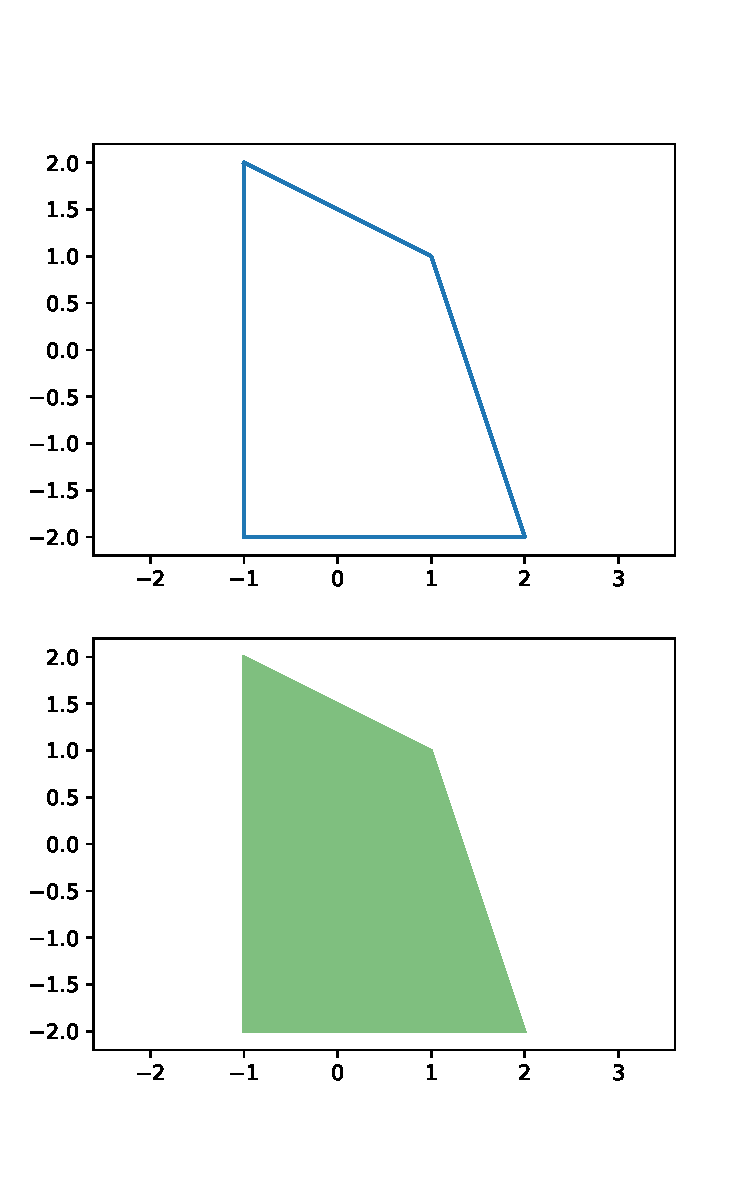
\includegraphics[width=.3\linewidth]{NN/input1_convex.pdf} &
		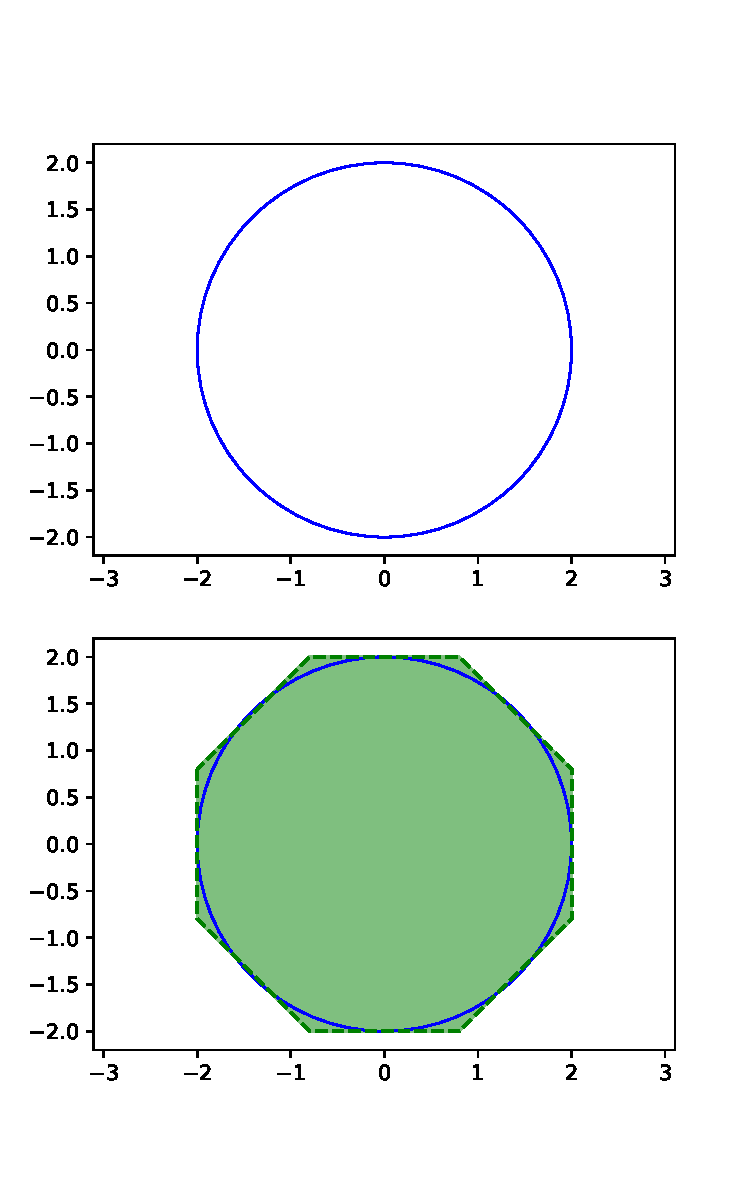
\includegraphics[width=.3\linewidth]{NN/input2_approx.pdf} &
		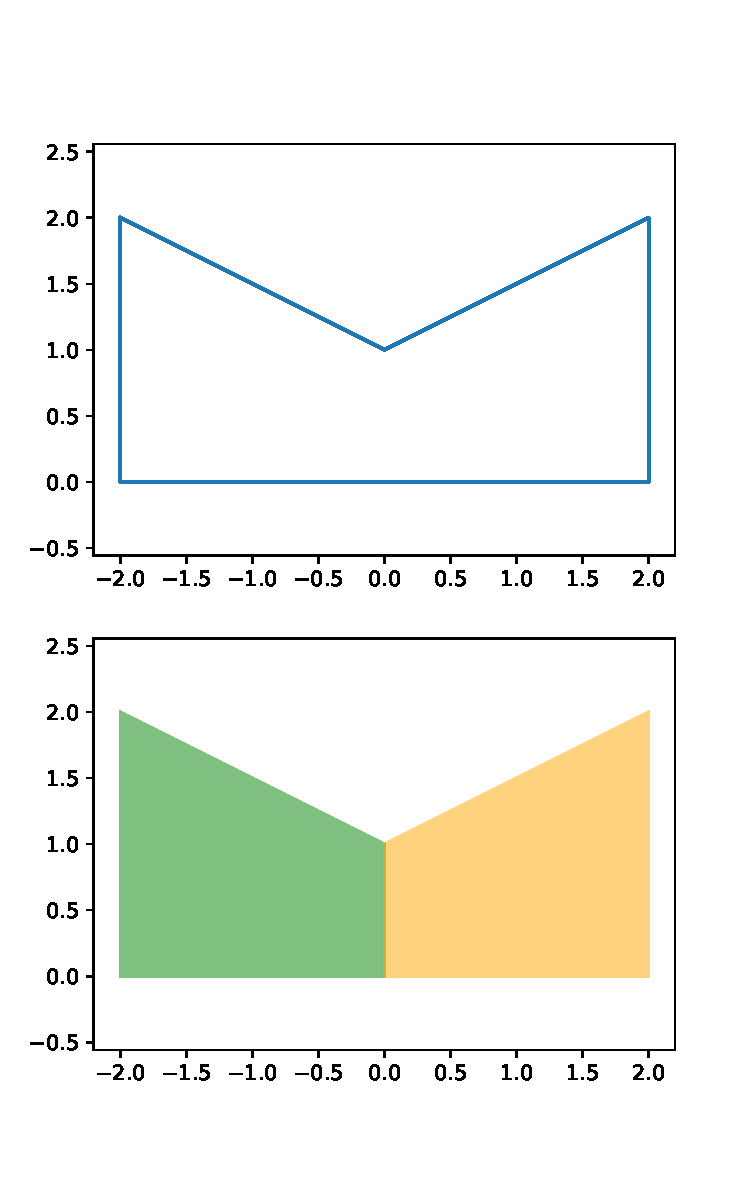
\includegraphics[width=.3\linewidth]{NN/input3_split.pdf}
	\end{tabular}
\end{figure}

Given our choice of abstract domain and a concrete network $\nu :
I \to O$ with $I \subset \mathbb{R}^n$ and $O \subset \mathbb{R}^m$,
we need to show how to obtain an \emph{abstract neural network}
$\tilde{\nu} : \langle I \rangle \to \langle O \rangle$ that provides
a sound overapproximation of $\nu$. To frame this concept, we
introduce the notion of consistent abstraction.

\begin{definition}{(Consistent abstraction)}
\normalfont Given a mapping $\nu : \mathbb{R}^n \to \mathbb{R}^m$, a 
mapping $\tilde{\nu} : \langle \mathbb{R}^n \rangle \to \langle 
\mathbb{R}^m \rangle$, abstraction function $\alpha : 2^{\mathbb{R}^n} 
\to \langle \mathbb{R}^m \rangle$ and concretization function 
$\gamma : \langle \mathbb{R}^m \rangle \to 2^{\mathbb{R}^m}$,
the mapping $\tilde{\nu}$ is a consistent abstraction of $\nu$ over a 
set of inputs $X \subseteq I$ exactly when 
\begin{equation}
\label{eq:cons}
\{ \nu(x) \mid x \in X \} \subseteq \gamma(\tilde{\nu}(\alpha(X)))
\end{equation}
\end{definition}

The notion of consistent abstraction can be readily extended to
families of sets as follows. The mapping $\tilde{\nu}$ is a consistent
abstraction of $\nu$ over a family of sets of inputs $X_1 \ldots X_p$
exactly when 
\begin{equation}
\label{eq:consset}
\{ \nu(x) \mid x \in \cup_{i=1}^p X_i \} \subseteq
\gamma(\tilde{\nu}(\alpha(X_1, \ldots, X_p)))
\end{equation}
where we abuse notation and denote with $\tilde{\nu}(\cdot)$
the family 
$\{ \tilde{\nu}(P_1), \ldots, \tilde{\nu}(P_s) \}$ with
$\{P_1, \ldots, P_s\} = \alpha(X_1, \ldots X_p)$

To represent polytopes and define the computations performed by
abstract layers we resort to a specific subclass of \emph{generalized star
sets}, introduced in~\cite{bak2017simulation} and defined as
follows --- the notation is adapted from~\cite{tran2019star}.

\begin{definition}{(Generalized star set)}
  \normalfont Given a \emph{basis matrix}
  $V \in \mathbb{R}^{n \times m}$ obtained arranging a set of
  $m$ \emph{basis vectors} $\{v_1, \ldots v_m\}$ in columns , a point
  $c \in \mathbb{R}^n$ called \emph{center} and a \emph{predicate} $R 
  : \mathbb{R}^m \to \{\top, \bot\}$, a generalized star set is a
  tuple $\Theta = (c,V,R)$.
  The set of points represented by the generalized star set is given by 
  \begin{equation}
    [ \! [ \Theta  ] \! ]  \equiv \{z \in \mathbb{R}^n \mid z = Vx + c
    \mbox{ such that } R(x_1, \ldots, x_m) = \top\}
  \end{equation}
\end{definition}

In the following we denote $[\![ \Theta ]\!]$ also as
$\Theta$. Depending on the choice of $R$, generalized star sets can
represent different kinds of sets, but 
we consider only those such that $R(x) := Cx \leq d$, where $C \in
\mathbb{R}^{p \times m}$ and $d \in \mathbb{R}^p$ for $p \geq 1$,
i.e., $R$ is a conjunction of $p$ linear constraints
as in~\cite{tran2019star}; we further require that the set $Y = \{y \in
\mathbb{R}^m \mid C y \leq  d\}$ is bounded. 

\begin{proposition}
\label{prop:polistar}
Given a generalized star set $\Theta = (c,V,R)$ such that
$R(x) := Cx \leq d$ with $C \in \mathbb{R}^{p \times m}$ and
$d \in \mathbb{R}^p$, if the set $Y
= \{y \in \mathbb{R}^m \mid C y \leq d\}$ is bounded, then the set of
points represented by  $\Theta$ is a polytope in $\mathbb{R}^n$, i.e.,
$\Theta \in \langle \mathbb{R}^n \rangle$. 
\end{proposition}

The proof of proposition (\ref{prop:polistar}) is
straightforward, since the set $Y$ is a polytope in $\mathbb{R}^m$, 
the mapping  $Vx + c$ is an affine mapping from  $\mathbb{R}^m$ to
$\mathbb{R}^n$ and affine mappings of polytopes are still
polytopes. From~\cite{tran2019star} we know that polytopes can be
represented as generalized star sets, and thus our 
restricted form of star sets provides an equivalent representation  
of polytopes in $\mathbb{R}^n$; in the following, we refer
to generalized star sets obeying our restrictions simply as \emph{stars}.

The simplest abstract layer to obtain is the one abstracting affine
transformations. As we have already mentioned, affine transformations
of polytopes are still polytopes, so we just need to define how to
apply an affine transformation to a star --- the definition is
adapted from~\cite{tran2019star}.  

\begin{definition}
  \label{def:absaffine} (Abstract affine mapping)
  \normalfont Given a star set $\Theta = (c,V,R)$ and an affine
  mapping $f : R^n \to R^m$ with $f = Ax + b$, the abstract affine
  mapping $\tilde{f} : \langle R^n \rangle \to \langle R^m \rangle$
  of $f$ is defined as $\tilde{f}(\Theta) = (\hat{c},\hat{V},R)$ where 
  \begin{equation*}
    \hat{c} = Ac + b \qquad \hat{V} = AV 
  \end{equation*}
\end{definition}

Intuitively, the center and the basis vectors of the input star
$\Theta$ are affected by the transformation of $f$, while the
predicates remain the same.

\begin{proposition}
\label{prop:affinecons}
Given an affine mapping $f : \mathbb{R}^n \to \mathbb{R}^m$, the
corresponding abstract mapping $\tilde{f} : \langle
\mathbb{R}^n \rangle \to \langle \mathbb{R}^m \rangle$ provides a consistent
abstraction over any bounded set $X \subset \mathbb{R}^n$, i.e.,
$\{ f(x) \mid x \in X \} \subseteq \gamma(\tilde{f}(\alpha(X)))$ for
all $X \subset \mathbb{R}^n$. 
\end{proposition}

To prove proposition (\ref{prop:affinecons}), we observe that
the set $\alpha(X)$ is any polytope $P$ such that $P \supseteq \mathcal{C}(X)$
--- equality holds only when $X$ is already a polytope, and thus $X
\equiv \mathcal{C}(X) \equiv P$. Let $\Theta_P = (c_P,V_P,R_P)$ be the
star corresponding to $P$ defined as
\begin{equation*}
c_P = 0^n \qquad V_P = I^n \qquad R_P = C_Px + d_P \leq 0
\end{equation*}
where $0^n$ is the $n$-dimensional zero vector, and $I^n$ is the $n
\times n$ identity matrix --- the columns of $I^n$ correspond
to the standard orthonormal basis $e_1, \ldots, e_n$ of
$\mathbb{R}^n$, i.e., $\lVert e_i \rVert = 1$ and $e_i \cdot e_j = 0$
for all $i \neq j$ with $i,j \in [1,n]$; the matrix $C_P \in
\mathbb{R}^{q \times n}$ and the vector $d_P \in 
\mathbb{R}^q$ collect the parameters defining $q$ half-spaces
whose intersection corresponds to $P$. Given our choice of $c$ and
$V$, it is thus obvious that $\Theta_P \equiv P$. Recall that $f = Ax + b$
with $A \in \mathbb{R}^{m \times n}$ and $b \in \mathbb{R}^m$; from  
definition (\ref{def:absaffine}) we have that
$\tilde{f}(\Theta_P) = \hat{\Theta}_P$ with $\hat{\Theta}_P = (\hat{c}_P, \hat{V}_P, R_P)$ and
\begin{equation*}
\hat{c}_P = A 0^n + b = b \qquad \hat{V}_P = AI^n = A
\end{equation*}
The concretization of $\hat{\Theta}_P$ is just the set of
points contained in $\hat{\Theta}_P$ defined as
\begin{equation}
  \label{eq:affineconc}
\gamma(\hat{\Theta}_P) = \{ z \in \mathbb{R}^m \mid z = Ax  + b
\mbox{ such that } C_px \leq d_P \}
\end{equation}
Now it remains to show that $\{ f(x) \mid x \in X \} \subseteq
\gamma(\hat{\Theta}_P)$. This follows from the fact that, for a generic $y
\in \{ f(x) \mid x \in X \}$ there must exists $x \in X$ such that $y
= Ax + b$; since $x$ satisfies $C_p x \leq d_P$ by construction of
$P$, it is also the case that $y \in \gamma(\hat{\Theta}_P)$ by definition
(\ref{eq:affineconc}).

\section{ReLU abstraction algorithms}
\label{sec:relu_abst}

\begin{algorithm}[t!]
  \caption{Abstraction of the ReLU activation function.}
  \label{alg:relu-abst}
  \small
  \begin{algorithmic}[1]
    \Function{compute\_layer}{\emph{input} = $[\Theta_1, \ldots, \Theta_N]$, \emph{refine} = $[r_1, \ldots, r_n]$}
    \State \emph{output} = $[\:]$
    \For{$i = 1:N$} 
      \State \emph{stars} = $[\Theta_i]$
      \For{$j$ = $1:n$}
        \emph{stars} = \textsc{compute\_relu}(\emph{stars}, $j$,
        \emph{refine}$[j]$, $n$)
      \EndFor
      \State \textsc{append}(\emph{output}, \emph{stars})
    \EndFor
    \State \Return \emph{output}
    \EndFunction
  \item[]
    \Function{compute\_relu}{\emph{input} = $[\Gamma_1, \ldots,
        \Gamma_M]$, $j$, \emph{level}, $n$}
    \State $output$ = $[\: ]$
    \For{$k = 1:M$}
      \State $(lb_j, ub_j)$ = \textsc{get\_bounds}(\emph{input}$[k]$, $j$)
      \State $M = [e_1\ ...\ e_{j-1}\ 0\ e_{j+1}\ ...\ e_n]$
      \If {$lb_j \geq 0$} $S$ = \emph{input}$[k]$
      \ElsIf {$ub_j \leq 0$} $S$ = $M$ * \emph{input}$[k]$
      \Else
        \If{\emph{level} $>$ $0$}
          \State $\Theta_{low}$ = \emph{input}$[k] \wedge z[j] < 0$;
          \hspace{1ex}$\Theta_{upp}$ = \emph{input}$[k] \wedge z[j] \geq 0$
          \State $S$ = $[M \mbox{ * } \Theta_{low}, \Theta_{upp}]$
        \Else
          \State $(c,V,Cx \leq d)$ = \emph{input}$[j]$
          \State $C_1$ = $[0\ 0\ ...\ -1] \in \mathbb{R}^{1 \times m+1}$, $d_1 = 0$
          \State $C_2$ = $[V[j,:]\ -1] \in \mathbb{R}^{1 \times m+1}$, $d_2 = -c_k[j]$
          \State $C_3$ = $[\frac{-ub_j}{ub_j - lb_j} \cdot V[j,:]\ -1] \in \mathbb{R}^{1 \times m+1}$, $d_3 = \frac{ub_j}{ub_j - lb_j} (c[j] - lb_j)$
          \State $C_0$ = $[C\ 0^{m \times 1}]$, $d_0 = d$
          \State $\hat{C}$ = $[C_0;\ C_1;\ C_2;\ C_3]$, $\hat{d} = [d_0;\ d_1;\ d_2;\ d_3]$
          \State $\hat{V} = MV$, $\hat{V} = [\hat{V}\ e_j]$
          \State $S$ = $(Mc, \hat{V}, \hat{C} \hat{x} \leq \hat{d})$
        \EndIf
      \EndIf
      \State \textsc{append}($output$, S)
    \EndFor
    \State \Return $output$
    \EndFunction
  \end{algorithmic}
\end{algorithm}

Algorithm~\ref{alg:relu-abst}~\cite{guidotti2021pynever} defines 
the abstract mapping of a functional layer with $n$ ReLU activation 
functions and adapts the methodology proposed in~\cite{tran2019star}. 
The function \textsc{compute\_layer} takes as input an indexed list 
of $N$ stars $\Theta_1, \ldots, \Theta_N$ and an indexed list of $n$ 
positive integers called \emph{refinement levels}. For each neuron, 
the refinement level tunes the grain of the abstraction: level $0$
corresponds to the coarsest abstraction that we consider --- the
greater the level, the finer the abstraction grain. In the case of
ReLUs, all non-zero levels map to the same (precise) refinement, i.e.,
a piecewise affine mapping. The output of function
\textsc{compute\_layer} is still an indexed list of stars, that can be
obtained by independently processing the stars in the input list.
For this reason, the \textbf{for} loop starting at line 3
can be  parallelized to speed up actual implementations. 

Given a single input star $\Theta_i \in \langle R^n \rangle$, each 
of the $n$ dimensions is processed in turn by the \textbf{for} loop 
starting at line 5 and involing the function \textsc{compute\_relu}. 
Notice that the stars obtained processing the $j$-th dimension are 
feeded again to \textsc{compute\_relu} in order to process the 
$j+1$-th dimension. For each star given as input, the
function \textsc{compute\_relu} first computes the lower and upper
bounds of the star along the $j$-th dimension by solving two
linear-programming problems --- function \textsc{get\_bounds} at line
11. Independently from the abstraction level, if $lb_j \geq 0$ then
the ReLU acts as an identity function (line 13), whereas if $ub_j \leq
0$ then the $j$-th dimension is zeroed (line 14). The $\ast$ operator
takes a matrix $M$, a star $\Gamma = (c, V, R)$ and returns the star
$(Mc, MV, R)$. In this case, $M$ is composed of the standard orthonormal
basis in $\mathbb{R}^n$ arranged in columns, with the exception of 
the $j$-th dimension which is zeroed. 

\subsection{Exact abstract propagation}

When $lb_j < 0$ and $ub_j > 0$ we consider the refinement level. 
For any non-zero level, the input star is ``split” into two new stars, 
one considering all the points $z < 0$ ($\Theta_{low}$) and the other 
considering points $z \geq 0$ ($\Theta_{upp}$) along dimension $j$. 
Both $\Theta_{low}$ and $\Theta_{upp}$ are obtained by adding to the 
input star \textit{input[k]} the appropriate constraints. 
If the analysis at lines 17–18 is applied throughout the network, 
and the input abstraction is precise, then the abstract output 
range will also be precise, i.e., it will coincide with the concrete one: 
we call complete the analysis of \nevertwo{} in this case. The number
of resulting stars is worst-case exponential, therefore the complete
analysis may result computationally infeasible.

\begin{proposition}
\label{prop:relucons}
Given a ReLU mapping $f : \mathbb{R}^n \to \mathbb{R}^n$, the
corresponding abstract mapping $\tilde{f} : \langle
\mathbb{R}^n \rangle \to \langle \mathbb{R}^n \rangle$ defined in 
Algorithm~\ref{alg:relu-abst} provides a consistent 
abstraction over any bounded set $X \subset \mathbb{R}^n$, i.e.,
$\{ f(x) \mid x \in X \} \subseteq \gamma(\tilde{f}(\alpha(X)))$ for
all $X \subset \mathbb{R}^n$. 
\end{proposition}

%\textbf{TODO: proof of the above}

\begin{proposition}
\label{prop:allcons}
Given a concrete network $\nu : \mathbb{R}^n \to \mathbb{R}^m$ comprised 
of a finite number $p$ of layers 
$f_1: \mathbb{R}^n  \to \mathbb{R}^{n_1}, \ldots, f_p: \mathbb{R}^{n_{p-1}} \to \mathbb{R}^{m}$ 
such that each $f_i$ is either an affine or functional layer implementing 
ReLUs, the corresponding abstract network
$\tilde{\nu} : \langle \mathbb{R}^n \rangle \to \langle \mathbb{R}^m \rangle$ 
comprised of the corresponding abstract layers 
$\tilde{f}_1: \langle \mathbb{R}^n \rangle  \to \langle \mathbb{R}^{n_1} \rangle, \ldots, 
\tilde{f}_p: \langle \mathbb{R}^{n_{p-1}} \rangle \to \langle \mathbb{R}^{m} \rangle$ 
provides a consistent abstraction over any bounded set $X \subset \mathbb{R}^n$, i.e.,
$\{ \nu(x) \mid x \in X \} \subseteq \gamma(\tilde{\nu}(\alpha(X)))$ for
all $X \subset \mathbb{R}^n$. 
\end{proposition}

Proposition~\ref{prop:allcons} enforces that we can prove the (local) robustness of
a neural network by propagating the abstraction of an input set representing the
$l_{\infty}$ ball around a given input with a small perturbation $\epsilon$ and check
whether the output set is large enough to cause a misclassification.

\begin{proposition}
\label{prop:halfspace-intersect}
The intersection of a star $\Theta = (c,V,R)$ and a half-space 
$\mathcal{H} = \{z | Hz \leq g\}$ is another star with the following characteristics:
$\overline{\Theta} = \Theta \cap \mathcal{H} = (\overline{c},\overline{V},
\overline{R})$ with $\overline{c} = c$, $\overline{V} = V$,
$\overline{R} = R \wedge R'$ and $R'(x) = (H V)x \leq g - H c$
\end{proposition}
The proof of the proposition is straightforward since it is analogous to 
adding new constraints to the predicate of the star, as done for the ReLU 
abstract transformer.

\begin{proposition}
\label{prop:safety}
Let $[\Theta_1, ..., \Theta_n]$ be a star set obtained by applying 
Algorithm~\ref{alg:relu-abst} to a network of interest $\nu$ and an input star set 
corresponding to the input component of the property of interest $P$. Moreover let 
$\mathcal{\hat{H}}$ be an half-space corresponding to the unsafe zone as defined 
by the property of interest. 
If $\overline{\Theta}_i = \Theta_i \wedge \mathcal{\hat{H}} = \emptyset$ for $i = 1, ..., n$ 
then the neural network $\nu$ satisfy the property $P$.
\end{proposition}

\begin{proposition}
\label{prop:counter-input-set}
If in Algorithm~\ref{alg:relu-abst} the stars were always refined for all 
neurons it is possible to compute the complete counter input set 
(\textit{i.e.}, the set containing all possible inputs that make the neural 
network unsafe) as $\mathcal{C}_{\Theta} = \bigcup_i (c, V, \overline{R}_i)$ 
where $\overline{R}_i$ are the predicates of the stars obtained by the 
intersection between the unsafe zone and the output star set, whereas $c$ 
and $V$ are the center and basis matrix of the input star. 
\end{proposition}

\begin{proof}
\label{proof:counter-input-set}
If the complete version of Algorithm~\ref{alg:relu-abst} is used then all 
the stars in the computation process are defined on the same predicate variables
$\textbf{x} = [x_1, ..., x_m]$ which do not change during the computations since 
only the number of constraints on $\textbf{x}$ is changed by the abstract
transformers. As consequence the $\overline{R}_i$ contain values of $\textbf{x}$ 
that make the network unsafe, moreover it also contains all the constraints of
the base predicate $R$ of the input star. Therefore the complete counter input 
set containing all possible inputs that make the neural network unsafe is
$\mathcal{C}_{\Theta} = \bigcup_i (c, V, \overline{R}_i)$, $\overline{R}_i \neq \emptyset$.
\end{proof}

\subsection{Over-approximate abstract propagation}
\label{subsec:relu-overapprox}

If the refinement level is $0$, then the ReLU is abstracted using 
the over-approximation proposed in~\cite{tran2019star} and 
depicted in Figure~\ref{fig:relu-overapprox}. This approach is 
much less conservative than others, i.e., based on zonotopes or 
abstract domains, and provides a tighter abstraction.

\begin{figure}
	\centering
	\caption{\label{fig:relu-overapprox} Graphical representation
		of the ReLU function (left) and the over-approximation 
		considering a single variable (right) with $lb_{j} = -2$ 
		and $ub_{j} = 2$.}
	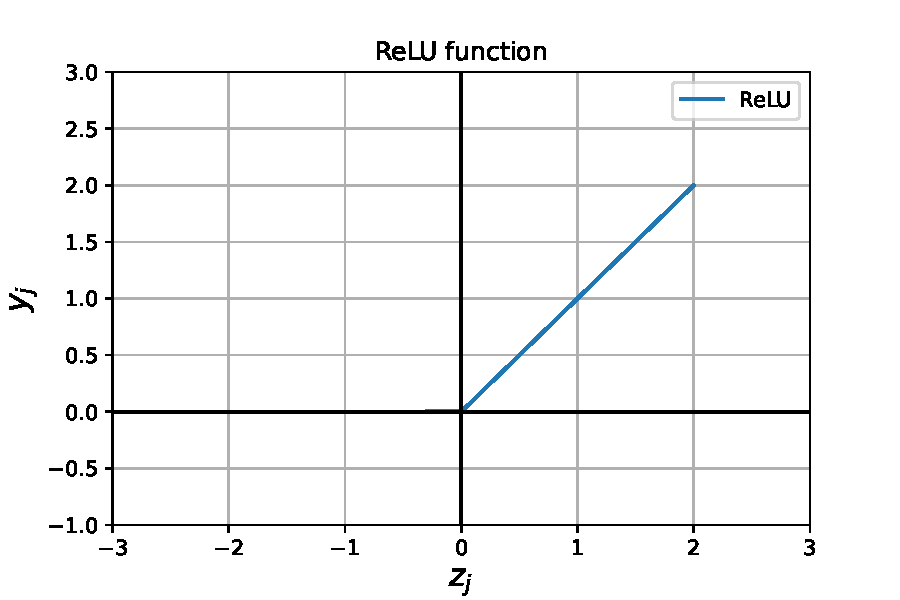
\includegraphics[width=.48\textwidth]{NN/ReLU_figure.pdf}
	\hspace*{\fill}
	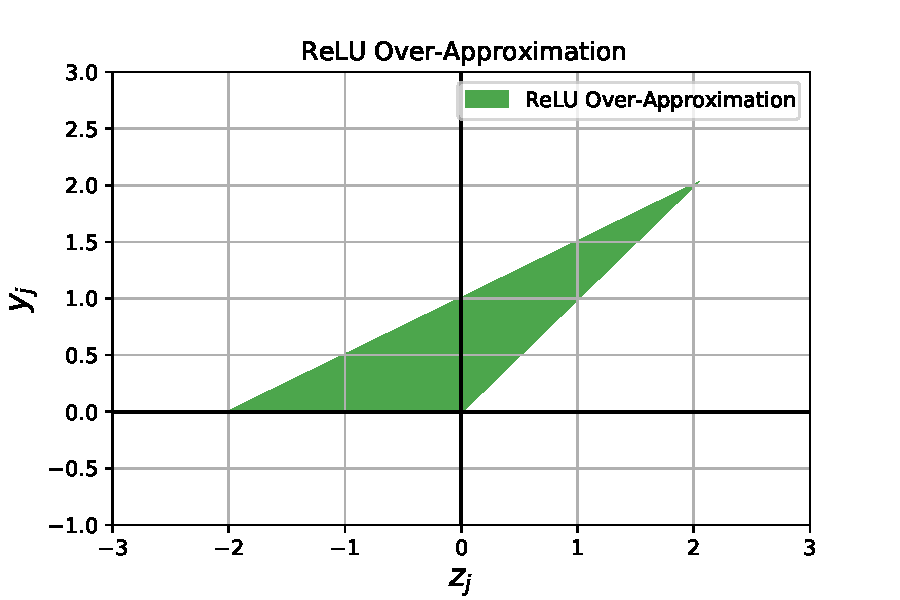
\includegraphics[width=.48\textwidth]{NN/relu_overapprox.pdf}
\end{figure}

As can be seen in Figure~\ref{fig:relu-overapprox}, three constraints
are needed to construct the over-approximation:
\begin{align*}
y_j &\geq 0\\
y_j &\geq z_j\\
y_j &\leq ub_j \frac{z_j - lb_j}{ub_j - lb_j}
\end{align*}
Such constraints must be added to the predicate matrix of the star, 
therefore we define an auxiliarly variable $x_{m+1}$ and we modify 
the basis matrix so that $y_j = x_{m+1}$ (line 26 in 
Algorithm~\ref{alg:relu-abst}). By doing so we make it possible to 
express our constraints only in terms of the predicate variables.
We remember that $z_j = V_j \mathbf{x} + c_j$, substituting it in 
the constraints we obtain:
\begin{align*}
x_{m+1} &\geq 0\\
x_{m+1} &\geq V_j \mathbf{x} + c_j\\
x_{m+1} &\leq ub_j \cdot \frac{V_j \mathbf{x} + c_j - lb_j}{ub_j - lb_j}
\end{align*}
If we reorder these constraints we can bring them in the format
$C\mathbf{x} \leq \mathbf{d}$:
\begin{align*}
- x_{m+1} &\leq 0\\
V_j \mathbf{x} - x_{m+1} &\leq -c_j\\
- \frac{ub_j}{ub_j-lb_j} V_j \mathbf{x} + x_{m+1} &\leq \frac{ub_j}{ub_j-lb_j}(c_j - lb_j)\\
\end{align*}
From these constraints it is straightforward to identify the 
corresponding matrices in lines 21 to 23 of the algorithm.

If this analysis is carried out throughout the network, then the 
output star will be a (sound) over-approximation of the concrete output 
range: we call \textit{over-approximate} the analysis of \nevertwo{} 
in this case. The number of star remains the same throughout
the analysis, but at the cost of a new predicate variable for each neuron
which, in turn, increases the complexity of the linear program required
by \textsc{get\_bounds}.

\subsection{Mixed abstract propagation}

In~\cite{guidotti2021pynever} it is proposed a new approach that adopts 
different levels of abstraction during the analysis: since each neuron
features its own refinement level, algorithm~\ref{alg:relu-abst}
controls the abstraction down to the single neuron. This setting strikes
a trade-off between complete and over-approximate settings. In order to
reduce as much as possible the approximation error, we rank the
neurons in each layer based on the area of the over-approximation
triangle depicted in Figure~\ref{fig:relu-overapprox}: intuitively,
the neuron with the widest bounds introduces a broader triangle and,
by design, a bigger approximation. 

We concretize the star along that neuron and propagate the approximate 
method along the others, such that each layer results in at most a single 
split. This reduces the computational cost significantly, as the growth 
becomes quadratic in the number of layers and the complexity increase by 
the approximation is contained. We call \textit{mixed} the analysis of 
\nevertwo{} in this case.
%\section{Improving abstract propagation}
\label{sec:optim}

\begin{figure}[t]
	\centering
	\caption{\label{fig:relu-subs} ReLU split subsumption example along axis $z_1$
		(the actual lower star is collapsed to a line)}
	\begin{subfigure}{.45\textwidth}
		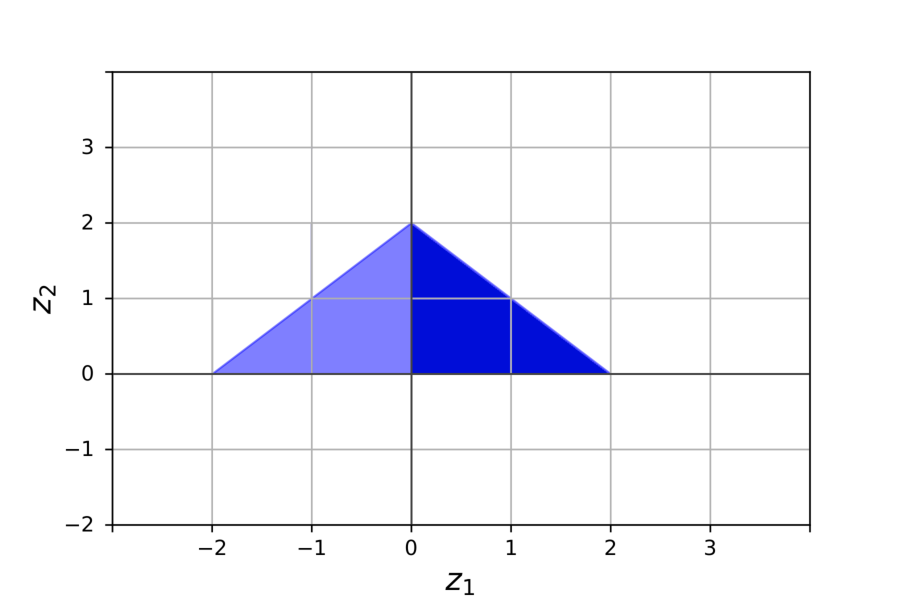
\includegraphics[width=\linewidth]{NN/Subsumed_true.pdf}
		\caption{\label{fig:relu-subs-ok}In this example the lower star can be
			subsumed by the upper one}
	\end{subfigure}
	\hspace*{\fill}
	\begin{subfigure}{.45\textwidth}
		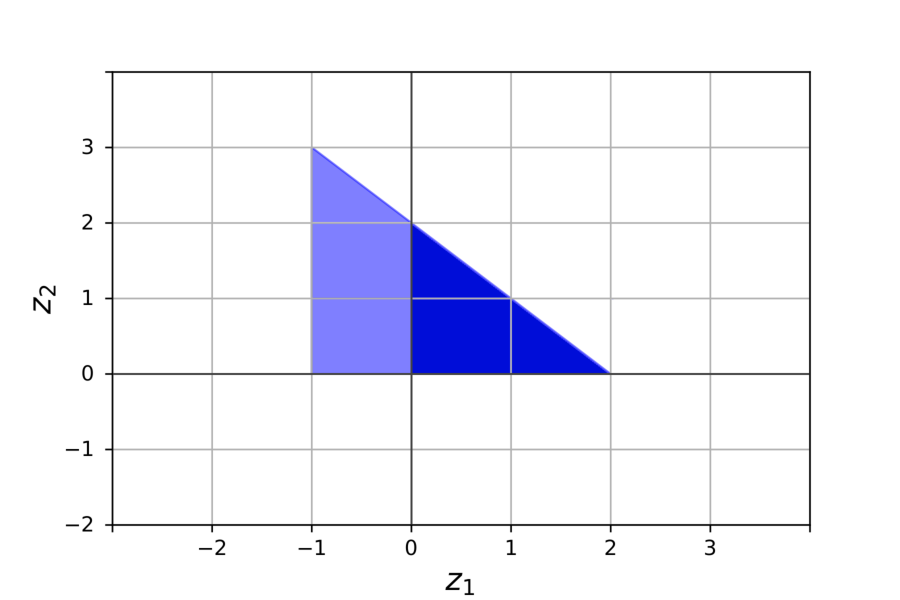
\includegraphics[width=\linewidth]{NN/Subsumed_false.pdf}
		\caption{\label{fig:relu-subs-no}In this example the lower star cannot be 
			subsumed by the upper one}
	\end{subfigure}
\end{figure}

The abstraction procedure detailed in Section~\ref{sec:abstr} allows to control the
number of stars produced during the layer propagation. Nevertheless, we can note that
the lower star in the ReLU split could be completely subsumed by the upper one depending
on the bounds along the other variables. 

Figure~\ref{fig:relu-subs} exemplifies this statement: in case~\ref{fig:relu-subs-ok}
the lower star is negligible when projected to the $z_2$ axis while in case~\ref{fig:relu-subs-no}
the projection adds information which is not present in the upper star. More formally,
we can say that if the lower star bounds along the dimension $z_2$ are lesser than the upper
star ones, then the upper star subsumes the lower on dimension $z_2$. We can generalize by
stating that for the dimension, i.e., neuron $i$ we can ignore the lower star if and only if
for all other dimensions, i.e., neurons $j = 1, ..., n$, $i \neq j$:

$$ub^j_{upp} \leq ub^j_{low} \wedge lb^j_{upp} \geq lb^j_{low}$$

The procedure is sound because the star set we obtain by the \textsc{compute\_relu} function
with the exact method in the same layer is guaranteed to contain stars with the same number
of dimensions such that the comparison is possible. Furthermore, given that ReLU does not
perform affine transformations, all stars share the same center and the dimension in the basis
matrix which is zeroed corresponds to the projection of the lower star on that dimension.

\begin{algorithm}[t]
	\caption{Star elimination algorithm}
	\label{alg:prop_v2}
	\begin{algorithmic}[1]
		\Function{get\_unique}{\emph{lower}, \emph{upper}, \emph{v}}
		\State $lower.lb_v = lower.ub_v = 0$
		\State $upper.lb_v = 0$
		\State \emph{dim\_list} = \textsc{order}(\emph{tot\_vars}, \emph{v})
		
		\For{$j$ in \emph{dim\_list}}
		\State $lb\_low_j, ub\_low_j$ = \textsc{get\_bounds}(\emph{lower}, $j$)
		\State $lb\_upp_j, ub\_upp_j$ = \textsc{get\_bounds}(\emph{upper}, $j$)
		
		\If{$ub\_upp > ub\_low$ or $lb\_upp < lb\_low$}
		\State \Return [\emph{lower, upper}]
		\EndIf
		\EndFor
		
		\State \Return [\emph{upper}]
		\EndFunction
		
		\item[]
		
		\Function{order}{\emph{num\_vars}, \emph{j}}
		\State \emph{output} = $[\:]$
		\For{$i = j + 1:num\_vars$}
		\State \textsc{append}(\emph{output}, $i$)
		\EndFor
		\For{$i = 0:j - 1$}
		\State \textsc{append}(\emph{output}, $i$)
		\EndFor
		\State \Return \emph{output}
		\EndFunction
		
		\item[]
		
		\Function{compute\_relu}{\emph{input} = $[\Gamma_1, \ldots,
			\Gamma_M]$, $j$, \emph{level}, $n$}
		
		$\ldots$
		
		\If{\emph{level} $>$ $0$}
		\State $\Theta_{low}$ = \emph{input}$[k] \wedge z[j] < 0$;
		\hspace{1ex}$\Theta_{upp}$ = \emph{input}$[k] \wedge z[j] \geq 0$
		\State $S$ = \textsc{get\_unique}($M \mbox{ * } \Theta_{low}, \Theta_{upp}, j$)
		\EndIf
		
		$\ldots$
		
		\EndFunction
	\end{algorithmic}
\end{algorithm}

Algorithm~\ref{alg:prop_v2} details the procedure for checking the elimination of
the lower star. In order to contain the number of LPs to solve, since each dimension
is processed subsequently, we start checking the dimensions following the one 
alongside which the ReLU split occurred: in this way, even if the check fails, the
LP does not add extra computational time as it is used for the next neuron. This
is obtained by function \textsc{order} in line $4$. 
After ordering the dimensions, we perform the subsumption check for each one of them;
whenever this check fails, both the lower and the upper star are returned without
spending further time checking other dimensions (line $9$). Only if the check is 
successful for every dimension, the function returns the upper star only (line $10$).
This modification is highlighted in the fragment of \textsc{compute\_relu} in lines
$18 - 22$. The cost for the extra LPs paid when the upper star subsumes the lower is 
balanced by the reduction of the number of stars that are propagated, whereas if the
subsumption check fails soon enough, no extra LPs are computed since the bounds are
used in the next neuron computation. The worst case scenario is a check that takes
almost all the dimensions to finally fail, which leads eventually to a major overhead.

%*******************************************************************************
%*********************************** PART 2 ************************************
%*******************************************************************************
\part{Bound Propagation}
%
\chapter{Bound Propagation Introduction}
\label{ch:bp-introduction}
\section{Bound propagation types}
\label{sec:bp_types}

The main goal of this chapter is to explain how we can apply a bound propagation on a Neural Network, made up of only fully connected layers at first, then also ReLU layers. Assume we have a property that set up an upper and lower bound for each neuron of the input. Essentially, let $\textbf{x}$ be the set of input neurons and $x_i$ the i-th neuron of $\textbf{x}$.
We can apply different types of bound propagation. The first that will be dealt with is the \textbf{naive propagation}. 

\subsection{Naive Propagation}

\begin{figure}[t]
	\caption{\label{fig:naive_prop} Example of naive propagation}
	\centering
	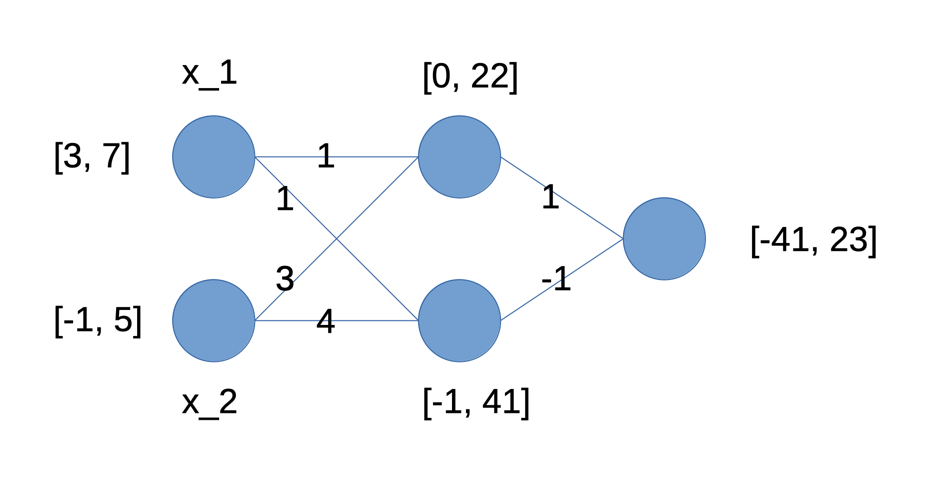
\includegraphics[scale= 0.3]{Chapter5/img/bound-propagation/naive_prop.png}
\end{figure}

In Fig~\ref{fig:naive_prop} represents a neural network consisting of two layers fully connected.\\
By performing the products and sums between the intervals and the fully connected weights along the layers we get an output interval [-41, 23].\\
Let the affine mapping (fc) be defined as  $\textbf{y} = W\textbf{x} + \textbf{b}$
and $W^+$ and $W^-$ be the positive and negative entries of $W$.\\
We also define $l^{+}_i$ and $l^{-}_i$ respectively as the vectors of the upper bounds and of the lower bounds.  

For calculating the intervals of the i-th fully connected layer for all nodes:

\begin{equation}
    \begin{aligned}
        lower\_bound\_i = W^+l^{-}_{i-1} + W^-l^{+}_{i-1} + b\\
        upper\_bound\_i = W^+l^{+}_{i-1} + W^-l^{-}_{i-1} + b
    \end{aligned}
\end{equation}

Now, note that the upper bound 23 of the output cannot be reached. It can appear only if the upper and lower nodes of the hidden layers are respectively 22 and -1 but this is impossible. This is because in order to have 22 in the upper node of the hidden layer it is necessary to have $x_1 = 7$ and $x_2 = 5$ as input values  but to have -1 in the lower node of the hidden layer it is necessary to have $x_1 = 3$ and $x_2 = -1$ at the same time. These two conditions are contradictory and therefore can't be satisfied, this is due to the fact that this is an overestimation of the real bounds. It is also an example of the \textbf{dependency problem}. 
Naive interval analysis suffers from large overestimation errors as it ignores the input dependencies during interval propagation.

\subsection{Symbolic Interval Propagation}

\begin{figure}[t]
	\caption{\label{fig:bound_prop}  Example of bound propagation}
	\centering
	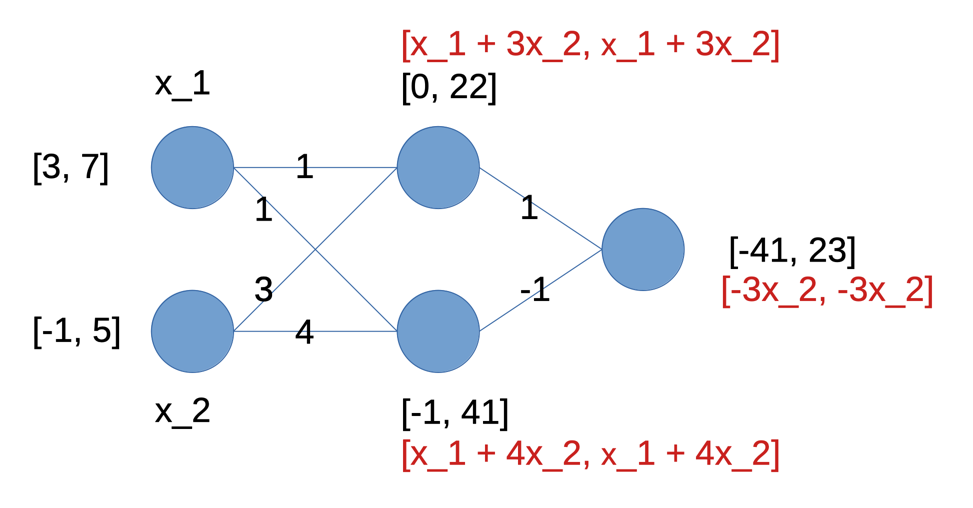
\includegraphics[scale= 0.3]{"Chapter5/img/bound-propagation/bound_prop_2.png"}
\end{figure}

In Fig~\ref{fig:bound_prop}  we use a different approach to overestimate the output interval. The main idea is to minimize overestimation by explicitly representing the intermediate computations of each neuron using symbolic intervals. These intervals encode the interdependency of the inputs and help in accurately estimating the output range of the neuron. In simpler terms, symbolic interval propagation is a technique that optimizes the calculation process within a neuron by using symbolic intervals to better understand the relationships between inputs and reduce the tendency to overestimate the output.\\
This approach on average, reduces significantly the over-approximation error with respect to the naive propagation.

\vspace{10mm}
In our example the intervals, made up respectively from a lower and an  upper bound vector, associated to the nodes of the input layers [$x\_1, x\_2$] are $l^{-}_0 = [3, -1]$ and $l^{+}_0 = [7,5]$.\\
Instead $[x_1 + 3x_2, x_1 + 3x_2]$ and [$x_1 + 4x_2, x_1 + 4x_2$] are the lower and upper symbolic bounds of the intermediate nodes.

Below are the procedure and formulas to compute the symbolic bounds of the i-th layer:
\begin{enumerate}
    \item For the input layer instantiate two identity matrix whose size is the number of input neuron and two zeroes offset vectors. In our example, we would instantiate 2 2x2 matrices and two zero-vectors of 2 elements.

        \begin{equation*}
            lower_0 = \begin{pmatrix}
            1 & 0 & \cdots & 0 \\
            0 & 1 & \cdots & 0 \\
            \vdots & \vdots & \ddots & \vdots \\
            0 & 0 & \cdots & 1
            \end{pmatrix}
        \end{equation*}
        
        \begin{equation*}
            upper_0 = \begin{pmatrix}
            1 & 0 & \cdots & 0 \\
            0 & 1 & \cdots & 0 \\
            \vdots & \vdots & \ddots & \vdots \\
            0 & 0 & \cdots & 1
            \end{pmatrix}
        \end{equation*}

        \begin{equation*}
            lower\_offset_0 = \begin{pmatrix}
            0  \\
            \vdots \\
            0  \\
            \end{pmatrix}
        \end{equation*}

        \begin{equation*}
            upper\_offset_0 = \begin{pmatrix}
            0  \\
            \vdots \\
            0  \\
            \end{pmatrix}
        \end{equation*}
        
    \item
    Let $upper_i$ and $lower_i$ respectively the matrix of the symbolic upper bound equations and lower bound equation of a fully connected layer i.
    A fully connected layer is characterised by a weight matrix $W$ and a bias vector $b$.\\
    Below are the formulas to calculate the upper symbolic bound and the lower symbolic bounds after a fully connected layer:
    \begin{equation}
        \begin{aligned}
            &lower_i = W^+_i lower_{i-1} + W^-_i upper_{i-1}\\
            &upper_i = W^+_i upper_{i-1} + W^-_i lower_{i-1}\\
            &lower\_offset_i = W^+_i lower\_offset_{i-1} + W^-_i upper\_offset_{i-1}\\
            &upper\_offset_i = W^+_i upper\_offset_{i-1} + W^-_i lower\_offset_{i-1}\\
        \end{aligned}
    \end{equation}
    where:\\
    $lower_{i-1}$ and $lower_{i-1}$ are the upper and lower symbolic bounds 
    matrixes of the previous layer. \\

    By iterating the above formula through all layers of a complete fully connected network, you get the symbolic upper and lower bounds equations for each fc layer.

    Given the symbolic upper and lower bounds matrices $lower\_i$, $upper\_i$, $lower\_offset_i$ and $upper\_offset_i$ of layer $i$ and a couple of vectors (the upper and lower bound vector $l^{+}_0$ $l^{-}_0$ ) on the input layer you can calculate the \textbf{numeric} lower and upper bounds of layer $i$. The formulas are below:
    
     \begin{equation}
        \begin{aligned}
            &numeric\_lower_i = lower_{i}^{+} \cdot l^{-}_0 + lower_{i}^{-} \cdot l^{+}_0 + offset_i\\
            &numeric\_upper_i = upper_{i}^{+} \cdot l^{+}_0 + lower_{i}^{-} \cdot l^{-}_0 + offset_i\\
        \end{aligned}
    \end{equation}

    where: \\
     $numeric\_lower_i$ and $numeric\_upper_i$ are the lower and upper numeric bounds vectors of layer $i$\\
     $l^{-}_0$ and $l^{+}_0$ are the lower and upper bounds vectors of input layer\\
\end{enumerate}

By iterating this process for all layers, we get the numeric and numeric bounds for all the layer of the network.\\
The main problem that arises is that we often need to deal with networks formed by FC and ReLU. The rectified linear activation function or ReLU for short is a piecewise linear function that will output the input directly if it is positive, otherwise, it will output zero. But we can't deal with it because it is not a linear and, therefore, we have to use a convex approximation to deal with it.


\subsection{Iterative Refinement Propagation}

\begin{figure}[t]
	\caption{\label{fig:iterative_propagation} Example of bisection and refinement}
	\centering
	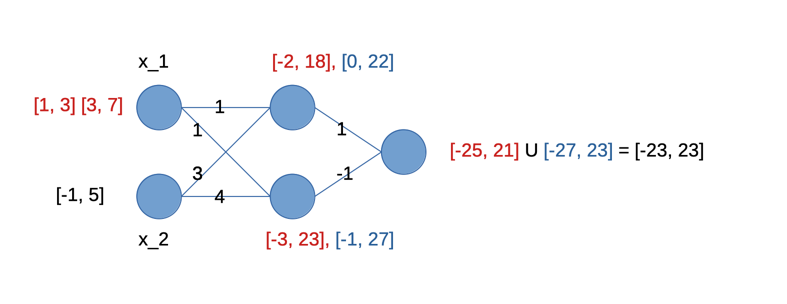
\includegraphics[scale=0.6]{"Chapter5/img/bound-propagation/bisection.png"}
\end{figure}

In fig~\ref{fig:iterative_propagation},  the input interval on a node is divided into two adjacent sub-intervals of equal size, effectively cutting it in half. This division helps decrease the overestimation and allows us to narrow down the range of possible values for the output. As a matter of fact the output interval is tighter respect to the one got with the naive propagation. It's important to note that we can continue refining the output interval by repeatedly splitting the input intervals in order to further tighten the overapproximation. This process is easily parallelizable because each split sub-interval can be independently checked.


    

	

	





\section{ReLU's Over-approximation}

The Rectified Linear Unit (ReLU) activation function is a commonly used activation function in neural networks. It is defined as follows:

\vspace{5mm}
$ReLU(x) = max(0, x)$
\vspace{5mm}
\\
In other words, if the input to the ReLU function (x) is greater than zero, the output will be equal to the input. If the input is less than or equal to zero, the output will be zero.
\\
The ReLU function has a simple and computationally efficient implementation, which contributes to its popularity. It introduces non-linearity into the network, allowing neural networks to learn complex relationships between inputs and outputs. ReLU is particularly useful in deep neural networks as it helps alleviate the vanishing gradient problem, where gradients become very small during backpropagation, by allowing the gradient to flow more easily for positive inputs.

\begin{figure}[t]
	\caption{\label{fig:relu_types} Main used ReLU's convex approximation in the literaturet}
	\centering
	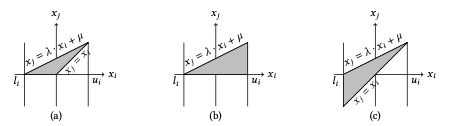
\includegraphics[scale=0.8]{"Chapter5/img/ReLU's/relus.png"}
\end{figure}


With regard to symbolic interval bound propagation the main problem that arises is that we often need to deal with networks formed by FC and ReLU. But we can't deal with it because it is not a linear and, therefore, we have to use a convex over-approximation. Below the main used convex over-approximation:

\begin{enumerate}
    \item The approximation of Fig. 4 (a) minimizes the area in the $x_i$ , $x_j$ plane, and would add the following relational constraints and concrete bounds for $x_j$:
       \begin{equation}
            \begin{aligned}
                & x_i \leq x_j, 0 \leq x_j, \\
                & x_j \leq u_i\left(x_i-l_i\right) /\left(u_i-l_i\right) . \\
                & l_j=0, u_j=u_i .
            \end{aligned}
        \end{equation}
        
 This ReLU approximation is the best possible in term of area but it has the disadvantage that uses 2 lower constraints. For this reason it is not well suitable for a further implementation in a bound propagation alghoritm.

    \item The approximation from Fig. 4 (b) adds the following constraints and bounds for $x_j$ :
    \begin{equation}
        \begin{aligned}
            & 0 \leq x_j \leq u_i\left(x_i-l_i\right) /\left(u_i-l_i\right), \\
            & l_j=0, u_j=u_i .
        \end{aligned}
    \end{equation}

    \item The approximation from Fig. 4 (c) adds the following constraints and bounds:
    \begin{equation}
        \begin{aligned}
            x_i & \leq x_j \leq u_i\left(x_i-l_i\right) /\left(u_i-l_i\right), \\
            l_j & =l_i, u_j=u_i .
        \end{aligned}
    \end{equation}
\end{enumerate}

\subsection{Application of ReLU approximation to bound propagation}
The networks used for verification purposes are typically small and typically consist of fully connected layers and ReLU activation layers. Earlier, we explained the process of bound propagation for networks composed solely of fully connected layers, referred to as Symbolic Interval propagation. Now, let's discuss how to modify the bound propagation method to make it compatible with ReLU layers.

Consider a network composed of three fully connected (FC) layers with dimensions 2x2, along with two ReLU layers, as shown in Figure 5 of the paper titled "Optimized Symbolic Interval Propagation for Neural Network Verification."


\begin{figure}[t]
	\caption{\label{fig:fc_relu_network} Simple neural network with FC and ReLU}
	\centering
	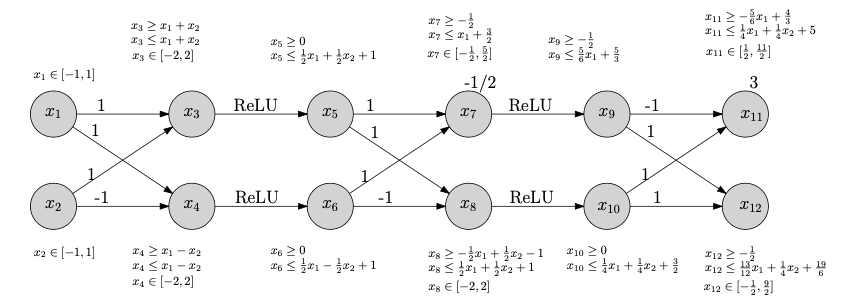
\includegraphics[scale=0.6]{"Chapter5/img/network_with_bound_prop/network_with_bound_prop.png"}
\end{figure}


To incorporate ReLU layers into the bound propagation process, we need to account for the behavior of the ReLU activation function. Below are the steps to modify bound propagation for networks containing ReLU layers:

\begin{enumerate}
	\item Symbolic Interval Propagation (SIP) with Fully Connected (FC) Layers:

	\begin{itemize}
		\item Initially, we start with an input layer, where the input bounds are represented symbolically.
		\item For each FC layer, we calculate the affine transformation symbolic bounds as seen previously.
		\item The numeric output bounds of the FC layer are obtained through the concretization operation of the symbolic bounds and input bounds
	\end{itemize}

	\item Incorporating ReLU layers:

		\begin{itemize}
			\item After each FC layer, introduce a ReLU layer, which applies the ReLU activation function element-wise to the output of the FC layer.
		\end{itemize}

	\item Bound Propagation through ReLU Layers

		\begin{itemize}
			\item For each ReLU layer, we compute the lower and upper bounds of the output based on the input bounds.
			\item If the lower bound of the input is greater than zero, the lower bound of the output remains the same as the lower bound of the input. This is intuitive because if the lower bound is greater that zero then we can ignore the ReLU 						second dial of the Carthesian plan and treat it as a simple bisector of the first quadrant.
			\item If the upper bound of the input is less than or equal to zero, the upper bound of the output is zero. This is intuitive because if the upper bound il less that zero than we can ignore the ReLU first dial of the Carthesian  plan and 						treat it as a simple zero function.
			\item If the lower bound is less than zero and the upper bound is greater than 0 then it is needed to apply an over-approximation of the ReLU symbolic bounds.\\
				In the example in the Fig ~\ref{fig:fc_relu_network} all the neurons are in the third case and it is used the following metric for the linearization:\\
				If $u<\lvert l \rvert$ is applied the ReLU over-approximation in Fig~\ref{fig:relu_types} b\\
				 Else If  $u>\lvert l \rvert$ is applied the ReLU over-approximationin in Fig~\ref{fig:relu_types} c\\
				This diversification in the over-approximation's choice is due to the fact that  if  $u<\lvert l \rvert$ the over-approximation in Fig~\ref{fig:relu_types} b introduces a smaller error than the one in  Fig~\ref{fig:relu_types} c and 						vice-versa. The over-approximation of the ReLU introduces a discrepancy between the symbolically propagated limits and the actual value limits, causing a potential over-estimation errors in limit propagation which increases as 						the number of ReLu layers increases and consequently as the depth of the network increases.
		\end{itemize}

	\item Iterative process:

		\begin{itemize}
			\item Apply the modified bound propagation process iteratively across all FC and ReLU layers in the network.
			\item The output bounds obtained from the last FC layer represent the output bounds of the network.
		\end{itemize}
\end{enumerate}

\subsection{Detailed Study of Symbolic Linear Relaxation of ReLU}
\label{subsec:symbolic-linear-relaxation}
The key insight of symbolic linear relaxation is to find the tightest linear bounds for the ReLU function, minimizing the overestimation error when approximating network outputs. However, it is important to note that the approximation errors may vary for overestimated nodes in different layers, depending on the symbolic intervals assigned as inputs.

For layers preceding the $n_0$-th layer, which is the first layer with overestimated nodes, all nodes have the same symbolic lower and upper bounds as you can notice in the first ReLU layer of the example.

However, in deeper layers where overestimated nodes become more frequent, the expressions for the lower and upper symbolic bounds can be more complex. To address this challenge, we provide a detailed discussion and illustration of how symbolic linear relaxation works.
The linearization below in not present in section 2, but it is the tightest linearization possible and it is the one that will be used in the bound propagation. This is due to the fact that it introduces the smallest error possible respect to the linearizations seen before.

Let's consider an arbitrary overestimated node A, with the equation given by $z = Relu(Eq)$, where $Eq$ represents its input kept as a symbolic interval $[Eq_{low}, Eq_{up}]$. Additionally, let $n_0$ represent the first layer where overestimated nodes occur, $n_A$ denote the layer in which node A appears, and $(l_{low}, u_{low})$ and $(l_{up}, u_{up})$ represent the concrete lower and upper bounds of A's symbolic bounds $Eq_{low}$ and $Eq_{up}$.

We can consider several cases for the symbolic linear relaxations applied to node A, depending on its position relative to the $n_0$ layer.
    
\begin{enumerate}
        \item if $n_0 == n_A$: if A is an overstimed node in $n_0$ than we see that A's input equation $Eq$ satisfies $Eq_{low} = Eq_{up}=Eq$ .  Due to the fact that $u>0$ and $l<0$ the output can be approximated with:
        \begin{equation}
       	 \operatorname{Relu}([E q, E q]) \mapsto\left[\frac{u}{u-l} E q, \frac{u}{u-l}(E q-l)\right]
        \end{equation}
        
        \item $n_A>n_0$ : If $\mathrm{A}$ is an overestimated node after $n_0$-th layer, 
    	possibly its symbolic lower bound equation $E q_{l o w}$ is no longer the same as its upper bound equation $E q_{u p}$ before relaxation.
     	Though we can still approximate the it as $\operatorname{Relu}\left(\left[E q_{l o w}, E q_{u p}\right]\right) \mapsto\left[\frac{u_{u p}}{u_{u p}-l_{l o w}} E q_{l o w}, \frac{u_{u p}}{u_{u p}-l_{l o w}}\left(E q_{u p}-l_{\text {low }}\right)\right]$, this is not 		 	the tightest 	possible bound. Therefore, we consider bounds on $E q_{l o w}$ and $E q_{u p}$ independently to achieve tighter approximations.
	\begin{equation}
    		\begin{aligned}
    			& \operatorname{Relu}\left(\left[E q_{\text {low }}, E q_{u p}\right]\right) \mapsto \\
    			& \qquad\left\{\begin{array}{l}
    				{\left[0, \frac{u_{u p}}{u_{u p}-l_{u p}}\left(E q_{u p}-l_{u p}\right)\right] \quad\left(l_{\text {low }} \leq 0, l_{u p} \leq 0, u_{l o w} \leq 0, u_{u p}>0\right)} \\
    				{\left[0, E q_{u p}\right] \quad\left(l_{\text {low }} \leq 0, l_{u p} \leq 0, u_{l o w}>0, u_{u p}>0\right)} \\
    				{\left[\frac{u_{l o w}}{u_{l o w}-l_{l o w}} E q_{l o w}, \frac{u_{u p}}{u_{u p}-l_{u p}}\left(E q_{u p}-l_{u p}\right)\right] \quad\left(l_{\text {low }} \leq 0, l_{u p}>0, u_{l o w} \leq 0, u_{u p}>0\right)} \\
    				{\left[\frac{u_{\text {low }}}{u_{\text {low }}-l_{l o w}} E q_{l o w}, E q_{u p}\right] \quad\left(l_{\text {low }} \leq 0, l_{u p} \leq 0, u_{l o w}>0, u_{u p}>0\right)}
   			\end{array}\right.
   		\end{aligned}
%    	
	\end{equation}
 \end{enumerate}
    
%\section{Counter-example Guided Abstraction Refinement}
\label{sec:cegar}

Our algorithm can be used to compute the complete or over-approximate 
reachable set of the neural network of interest. Once the reachable 
set has been computed, the property of interest can be verified by computing
the intersection between the negation of such property and the reachable 
set (which we call \textit{reachable counter set}). If such intersection is 
the empty set, then the network is compliant with the property of interest; 
otherwise, if the reachable set is complete, we have shown that the network 
is unsafe. However, if the reachable set is over-approximated, the concrete 
network may satisfy the property, and the over-approximation may be too coarse.
In both cases in which the reachable counter set is not the empty set, we are 
interested in extracting concrete input points corresponding to the output 
contained in the reachable counter set.
In particular, when we have a complete counter reachable set we can leverage 
the following theorem, adapted from~\cite{tran2020verification}:

\begin{theorem}
	\label{th:counter-input}
	Let $\nu$ be a feed-forward neural network, $\Theta = (c, V, R)$ be a star 
	input set, $\nu(\Theta) = \bigcup_{i=1}^k \Theta_i$, $\Theta_i = 
	(c_i, V_i, R_i)$ be the reachable set of the neural network and \emph{S} be a 
	safety specification. Denote $\overline{\Theta}_i = \Theta_i \cap \neg 
	\mathbf{S} = (c_i, V_i, \overline{P}_i)$, $i = 1, ..., k$. The neural network 
	is safe if and only if $\overline{P}_i = 0$ for all i. If the neural network 
	violates its safety property then the complete counter input set containing all 
	possible inputs in the input set that lead the neural network to unsafe states 
	is $\mathbf{C} = \bigcup_{i=1}^k (c, V, \overline{P}_i), \overline{P}_i \neq 0$.
\end{theorem}

For the proof of Theorem \ref{th:counter-input} we refer 
to~\cite{tran2020verification}.
Using Theorem~\ref{th:counter-input} we can easily compute the complete counter 
input set, so the problem of extracting concrete input points becomes the problem 
of extracting points from a star-set which in itself can be considered as 
extracting points from a single star. To do this, we consider the problem of 
extracting points from the predicate of the star, which, under our pre-conditions, 
is always a polytope. We will then apply to the points of the predicate ($\alpha$) 
the affine transformation $x = c + V \alpha$ to obtain a corresponding point of 
the star of interest. To extract the point from the polytope defined by the 
predicate, we leverage the hit and run sampler~\cite{DBLP:conf/wsc/Smith96}.
It should be noted that while the hit and run algorithm produces an approximation 
of a uniform distribution for the $\alpha$ of the predicate, the application of 
the affine transformation needed for the transformation to the point of the star 
skews such distribution. A possible solution to this issue is to transform the 
predicate to its V-representation, apply the affine transformation directly to the 
polytope, return to the H-representation and apply the hit and run sampler. 
However, for our aims, the skew of the distribution is not that relevant. 
Therefore, at least at this time, we do not need to transform between the two 
representations, which is computationally expensive.
%
The problem is different when we are working with the over-approximate reachable 
counter set: in this case, we do not have a way to compute the counter input set 
since the addition of the new variables needed for the over-approximation to the 
predicate of the star invalidates Theorem~\ref{th:counter-input}.
Therefore an alternative solution is needed to compute inputs that allegedly are 
not compliant with the property of interest. We define the \textit{abstract counter
	output set} (ACOS) as the intersection between the abstract reachable set and the
negation of the property $S$. Our algorithm extracts a point from the ACOS using hit 
and run sampling and then searches for the corresponding input point. Formally the 
search problem of the corresponding input point can be defined as:
\begin{definition}
	Given a reference output point $\hat{y}$, a starting input point $x$ and a feed 
	forward neural network $\nu$ we can define the search problem for the point 
	$\hat{x}$ which satisfies $\nu(\hat{x}) = \hat{y}$ as the following minimization 
	problem:
	\begin{equation*}
		\hat{x} = \min_{x} ||\hat{y} - \nu(x)||_2
	\end{equation*}
\end{definition}
However, the non-convexity and non-linearity of the function make the minimization 
problem not easily solvable: the non-convexity and the presence of 
local minima make it extremely difficult to apply gradient descent. 
Consequently, we developed a simple search-by-sampling algorithm which, given a 
starting point in the input space, generates a ``cloud" of points using a normal 
distribution with the starting point as center and a given variance. Such points 
are then compared, and the one whose corresponding output is nearest to the desired 
one is selected as the center for another step of the algorithm. The search terminates 
when the euclidean distance between the output found and the one we are searching for 
is less than a given threshold or when a given number of steps is exceeded.
If the algorithm finds an input point in the concrete input set and whose 
corresponding output is in the ACOS, we have found a concrete counter-example, and 
the network is proven unsafe. Otherwise, the point found is a point whose corresponding
output is reasonably close to the ACOS and can be leveraged for our refinement.
%
Once an adequate sample is found, we can use it to guide our refinement. 
The idea behind the refinement algorithm is to rank the approximation error
for each neuron by computing the triangle areas of the approximate method 
--- see, Section~\ref{sec:relu_abst} --- and enhance it with a measure of the 
relevance of the neurons with respect to the sample found. 
To compute the relevance, we leveraged the layer-wise relevance propagation 
algorithm~\cite{DBLP:journals/corr/SamekMBLM16} which, while traditionally used 
by the explainability community for classification models, can provide an adequate
relevance measure even for regression tasks. It should be noted that our 
implementation of the algorithm supports, at present, only fully-connected layers 
and ReLU activation functions. For more details on layer-wise relevance propagation 
we refer to~\cite{DBLP:series/lncs/MontavonBLSM19}. 
%
%
%
\begin{algorithm}[t]
	\caption{CEGAR Algorithm.}
	\label{alg:ref-abst}
	\begin{algorithmic}[1]
		\Function{cegar\_verification}{\emph{input\_set}, \emph{unsafe\_zone}, \emph{network}}
		\State \emph{ref\_levels} = $[0, ..., 0]$
		\State $ACOS$, $areas$, $safe$ = \textsc{starset\_ver}(\emph{input\_set}, \emph{unsafe\_zone}, \emph{network}, \emph{ref\_levels})
		\If {\textsc{is\_empty}(\emph{ACOS})}
		\State \Return $ACOS$, $areas$, $True$
		\EndIf
		\Statex
		\State $output\_counter$ = \textsc{get\_sample}(\emph{ACOS})
		\State $input\_counter$ = \textsc{input\_search}(\emph{network}, \emph{output\_counter})
		\If {$input\_counter \in input\_set$}
		\State \Return $ACOS$, $areas$, $False$
		\EndIf
		\Statex
		\State $neuron\_relevances$ = \textsc{compute\_rel}(\emph{input\_counter}, \emph{network})
		\State $ref\_levels$ = \textsc{compute\_ref\_levels}(\emph{neuron\_relevances}, \emph{areas})
		\State \Return \textsc{starset\_ver}(\emph{input\_set}, \emph{unsafe\_zone}, \emph{network}, \emph{ref\_levels})
		\EndFunction
	\end{algorithmic}
\end{algorithm}
%
%

The refinement procedure is detailed in Algorithm~\ref{alg:ref-abst}~\cite{DBLP:conf/cpsschool/DemarchiG22}.
As the first thing, it needs to apply our verification methodology in its
over-approximate form (line 3) to compute the over-approximate
reachable counter set and the triangle areas. If the network is proven to be safe 
(line 4) then the verification algorithm terminates (line 5), otherwise we can 
search the counter-example as shown before (line 6 and 7). 
If we found a concrete counter-example then the network is proven to be 
unsafe and the procedure terminates (line 8 and 9), otherwise we use the spurious
counter-example to find the relevances of the neurons of the network (line 10).
At this point, the relevances and the triangle areas can be used to evaluate the
significance of each ReLU neuron of the network. Once a measure of the significance 
is computed for each neuron of each ReLU layer, we can choose a given number of 
neurons to refine for each layer (line 11), and we can change the refinement levels
of Algorithm~\ref{alg:relu-abst} as needed. Then our verification methodology 
is applied again using the new refinement levels (line 12). Concerning the measure
of significance, we investigate on \emph{Product significance} (PS) which computes, 
for each neuron, the value of the multiplication between its relevance and the area
of the triangle abstraction, and \emph{mixed-R} (mR), which uses the relevances as 
coefficients for the ranking used in the standard mixed methodology.
%
%\chapter{PyNeVer BP Application}
\label{ch:bp-application}
\section{Bound Propagation applied to PyNeVer}
\label{sec:pynever_application}


The PyNeVer algorithm allows for property verification using different levels of refinement. The higher the level of refinement, the more efficient the algorithm becomes. However, as the level of refinement increases, the resulting polytope from the network will be larger than the real one, leading to decreased accuracy in the verification process.\\
Nevertheless, to achieve an exact computation of the output polytope for a given network and property, the minimum level of over-approximation must be used.\\
The objective of this thesis is to leverage bound propagation to improve the efficiency of the PyNeVer algorithm and achieve better time performance. The idea is to utilise bound propagation to determine the node bounds in advance, thereby reducing the number of calculations required during property verification. This will result in a more efficient solution by avoiding redundant computations and focusing only on the regions of interest.

%The GET_BOUNDS function is necessary to understand if a star at which is applied a ReLU function along the j-th dimension must be zeroes along that dimension if it has $ub_j<=0$, or directly propagated if $lb_j>=0$ or must be splitted along the j-th dim if $ub_j >=0 and lw_j<=0$.\\
%The GET_BOUNDS function is function that solves an optimization problem and it is quite expensive. The idea to make more efficient the algorithm is to apply a bound propagation algorithm before running the verification process. In this way it is possible to know a priori which neurons are stable .

\subsection{Real bounds and extimated bounds with bound propagation: all scenarios}
\label{subsec:all_bounds_scenarios}
 The bound propagation performs a calculation that return the numeric bound for all the fully connected layers on the network. Through the upper and lower bound of a neuron we can know if it is stable or unstable. The problem is that the bound propagation implemented must deal with ReLU functions which are not linear and hence introduces an over-approximation.
This implies:
\begin{equation}
	\begin{aligned}
		&lb^* < lb \\
		&ub^* > ub \\
	\end{aligned}
\end{equation}
where $lb$ and $ub$ are the real lower and upper bounds of a node, while $lb*$ and $ub*$ are the overestimated ones.\\
And this over-extimation grows up with the number of ReLU layers.\\
This over-extimation leads to different scenarios:
\begin{itemize}
	\item if the over-extimated lower bound of a node $lb*>0$, knowing that $lb>lb*$ then the neuron is for sure positive stable\\
		\begin{minipage}{\linewidth}
			\centering
			\includegraphics[width=\textwidth]{"Chapter6/img/pos_stable pos_stable"}
		\end{minipage}
	\item if the over-extimated upper bound of a node $ub*<0$, knowing that $ub<ub*$ then the neuron for sure negative stable\\
		\begin{minipage}{\linewidth}
			\centering
			\includegraphics[width=\textwidth]{"Chapter6/img/neg_stable neg_stable"}
		\end{minipage}
	\item if $lb*<0$ and $ub*>0$ knowing that $lb>lb*$ and $ub<ub*$ we cannot state if the neuron is stable or not. We can in turn distinguish three different cases:
	\begin{itemize}
		\item When $lb*<0$ and $lb>0$, in this case the bound propagation suggest that the neuron is unstable while in fact is positive stable\\
			\begin{minipage}{\linewidth}
				\centering
				\includegraphics[width=\textwidth]{"Chapter6/img/unstable pos_stable"}
			\end{minipage}
		\item When $ub*>0$ and $ub<0$, in this case the bound propagation suggests that the neuron is unstable while in fact is negative stable \\
			\begin{minipage}{\linewidth}
				\centering
				\includegraphics[width=\textwidth]{"Chapter6/img/unstable neg_stable"}
			\end{minipage}
		\item When $lb*<0, ub*>0$ and $lb<0, ub>0$, in this case the neuron is unstable as suggested by the bound propagation\\
			\begin{minipage}{\linewidth}
				\centering
				\includegraphics[width=\textwidth]{"Chapter6/img/unstable unstable"}
			\end{minipage}
	\end{itemize}
\end{itemize}
This means that the bound propagation states correctly if a neuron is positive or negative stable. Differently if it states that a neuron is unstable, it isn't possible to get useful information from it.


\subsection{Optimized version of PyNeVer with Bound Propagation}

As discussed earlier, the goal of this thesis is to apply bound propagation to optimize the code of pyNever. As discussed in SubSection \ref{subsec:all_bounds_scenarios}, through the precomputation of bound propagation, given a network and a property, it is possible to identify stable nodes without having to repeatedly call the GET\_BOUNDS function of pyNever. Below, an improved version of pyNever will be presented, which utilizes precalculated bounds to avoid using the GET\_BOUNDS function whenever possible. This enhances the efficiency of the program.

In Section \ref{subsec:all_bounds_scenarios}, we thoroughly examined the concept of bound propagation through precomputation. During this phase, bounds are computed for each node in the network, considering the specified property. The resulting bounds are then stored for later use during program execution.

The enhanced version of pyNever we will present leverages these precalculated bounds to avoid unnecessary calls to the GET\_BOUNDS function. Instead of invoking the function for each star and for each evaluated ReLU node, the program checks if the pre-computated bound states that the node is stable. If so, it is possible to avoid to call the GET\_BOUNDS function. If, differently, the precomputated bound states that the node is unstalbe then it will be necessary to calculate the exact bounds.  This optimization results in a significant improvement in overall performance.

The improved implementation of pyNever introduces an initial phase of bound precomputation, which takes time at program startup but greatly reduces execution time during the evaluation of subsequent nodes. Thanks to this strategy, a part of stable nodes can be efficiently identified without repeating costly computations for each evaluation.

The new version of pyNever, incorporating this improved implementation, offers a substantial advantage in terms of efficiency and execution speed. By minimizing calls to the GET\_BOUNDS function through the use of precalculated bounds, the program can handle large and complex networks more efficiently.

In conclusion, applying bound propagation with precomputed bounds in pyNever represents a significant advancement in code optimization. By utilizing precalculated bounds, the program can rapidly and efficiently identify stable nodes, avoiding redundant calculations and reducing overall execution time. This implementation offers a considerable advantage in the efficiency and usability of pyNever in various application contexts.

\begin{algorithm}[t!]
  \caption{Abstraction of the ReLU activation function with Bound Propagation.}
  \label{alg:new-relu-abst}
  \small
  \begin{algorithmic}[1]
    \Function{compute\_layer}{\emph{input} = $[\Theta_1, \ldots, \Theta_N]$, \emph{refine} = $[r_1, \ldots, r_n]$, \textbf{\emph{lower\_bounds: list}}, \textbf{\emph{upper\_bounds: list}}}
      \State \emph{output} = $[\:]$
      \For{$i = 1:N$} 
        \State \emph{stars} = $[\Theta_i]$
        \For{$j = 1:n$}
          \State \emph{stars} = \textsc{compute\_relu}(\emph{stars}, $j$, \emph{refine}$[j]$, $n$, \textbf{\emph{lower\_bounds[i]}}, \textbf{\emph{upper\_bounds[i]}})
        \EndFor
        \State \textsc{append}(\emph{output}, \emph{stars})
      \EndFor
      \State \Return \emph{output}
    \EndFunction

    \Function{compute\_relu}{\emph{input} = $[\Gamma_1, \ldots, \Gamma_M]$, $j$, \emph{level}, $n$, \textbf{\emph{lower\_bound}}, \textbf{\emph{upper\_bound}}}
      \State $output$ = $[\:]$
      \For{$k = 1:M$}
        \State $is\_positive\_stable$ = False
        \State $is\_negative\_stable$ = False
        \If {$lower\_bound \geq 0$}
          \State $is\_positive\_stable$ = True
        \ElsIf {$upper\_bound \leq 0$}
          \State $is\_negative\_stable$ = True
        \Else
          \State $(lb_j, ub_j)$ = \textsc{get\_bounds}(\emph{input}$[k]$, $j$)
        \EndIf
        \State $M = [e_1\ ...\ e_{j-1}\ 0\ e_{j+1}\ ...\ e_n]$
        \If {$is\_positive\_stable$}
          \State $S$ = \emph{input}$[k]$
        \ElsIf {$is\_negative\_stable$}
          \State $S$ = $M$ * \emph{input}$[k]$
        \ElsIf {$lb_j \geq 0$}
          \State $S$ = \emph{input}$[k]$
        \ElsIf {$ub_j \leq 0$}
          \State $S$ = $M$ * \emph{input}$[k]$
        \Else
          \If{\emph{level} $> 0$}
            \State $\Theta_{low}$ = \emph{input}$[k] \wedge z[j] < 0$;
            $\Theta_{upp}$ = \emph{input}$[k] \wedge z[j] \geq 0$
            \State $S$ = $[M \mbox{ * } \Theta_{low}, \Theta_{upp}]$
          \Else
            \State $(c,V,Cx \leq d)$ = \emph{input}$[j]$
            \State $C_1$ = $[0\ 0\ ...\ -1] \in \mathbb{R}^{1 \times m+1}$, $d_1 = 0$
            \State $C_2$ = $[V[j,:]\ -1] \in \mathbb{R}^{1 \times m+1}$, $d_2 = -c_k[j]$
            \State $C_3$ = $[\frac{-ub_j}{ub_j - lb_j} \cdot V[j,:]\ -1] \in \mathbb{R}^{1 \times m+1}$, $d_3 = \frac{ub_j}{ub_j - lb_j} (c[j] - lb_j)$
            \State $C_0$ = $[C\ 0^{m \times 1}]$, $d_0 = d$
            \State $\hat{C}$ = $[C_0;\ C_1;\ C_2;\ C_3]$, $\hat{d} = [d_0;\ d_1;\ d_2;\ d_3]$
            \State $\hat{V} = MV$, $\hat{V} = [\hat{V}\ e_j]$
            \State $S$ = $(Mc, \hat{V}, \hat{C} \hat{x} \leq \hat{d})$
          \EndIf
        \EndIf
        \State \textsc{append}($output$, $S$)
      \EndFor
      \State \Return $output$
    \EndFunction
  \end{algorithmic}
\end{algorithm}


\subsection{Pynever Complete Verification Example}

\begin{figure}[htbp]
  \centering
  \begin{minipage}[t]{0.4\textwidth}
    	\centering
   	\caption{\label{fig:nn_with_bp} non-bp-case}
	\includegraphics[scale=0.3]{"Chapter6/img/nn_with_bp"}
	\label{fig:nn_with_bp} 
  \end{minipage}
  
  \vspace{1cm}
  
  \begin{minipage}[t]{0.4\textwidth}
   	\centering
   	\caption{\label{fig:nn_without_bp} bp-case}
	\includegraphics[scale=0.3]{"Chapter6/img/nn_without_bp"}
	\label{fig:nn_without_bp}
  \end{minipage}

  \caption{Neural network composed by three FC and two ReLU layers}
  \label{fig:images}
\end{figure}


The Fig~\ref{fig:nn_without_bp} represents a NN composed by:s
\begin{itemize}
	\item Input: the NN has a two dimensional input
	\item FC1: a fully connected layer 2x4
	\item A ReLU activation function is applied to the FC1
	\item FC2: a fully connected layer 4x4 
	\item A ReLU activation function is applied to the FC2
	\item A FC3 4x2. The output is bidimensional
\end{itemize}

%The  FC1 and FC2 layers have the neurons colored in green or red:
%\begin{equation}
%    	\begin{aligned}
%    		& IF neuron color is \textit{green} \mapsto \textit{stable}
%    		& IF neuron color is \textit{red} \mapsto \textit{unstable} 
%    	\end{aligned}
%\end{equation}

In Fig~\ref{fig:nn_without_bp} it is represented a NN without a pre-applied bound propagation. The grey nodes which belongs to the FC layers are nodes whose stability or instability is not knows. Differently, in Fig~\ref{fig:nn_with_bp}, it is pre-applied a bound propagation. It is known a priori if green nodes are positive or negative stable, instead of grey nodes that might be stable or unstable.\\
Below is explained which are the differences and the advantages between the PyNeVer algorithm with bound propagation applied and the "normal" one:
\begin{itemize}
	\item bp-case: PyNeVer algorithm with bound propagation applied
	\item non-bp-case: PyNeVer algorithm without bound propagation applied. 
\end{itemize} 
The PyNeVer algorithm is sequential respect to the layers of the NN, this means that the verification process iterates from the first layer till the last one.
\begin{enumerate}
	\item FC1: the hyper-rectangle star defined by the input property is propagated through the FC1. For PyNeVer algorithm the number of stars in input in a fully connected layer  undergo a transformation (translation or rotation) but don't change in number. In our example we have one star in input in the FC1 layer and so we'll have one star in output. \textbf{The two algorithm versions behave in the same way for FC layers.}
	\item ReLU1:  for computing this layer PyNeVer calls COMPUTE\_LAYER function that, in our example, receives in input 1 star. COMPUTE\_LAYER function calls the function COMPUTE\_RELU one time for each dimension (the $i-th$ ReLU node corresponds to the $i-th$ dimension). \\
\textbf{For both the two algorithms}, the COMPUTE\_RELU bounds is called 4 times. The difference between the two algorithms is that the COMPUTE\_RELU in the non-bp-case must call the GET\_BOUNDS function for all stars along the j-th dimension while in the bp-case the GET\_BOUNDS is called only for the nodes we don't know if they are stable or unstable (the grey ones in fig~\ref{fig:nn_without_bp}). In this case the the bp-case the GET\_BOUNDS function is called 2 times while in the nn-bp-case it is called 4 times.  The max number of output stars is $2^{n_1}$ where $n_1$ is the number of nodes in a generic ReLU layer for each star in input.
	\item FC2: all the input stars undergo a transformation, but the number remains invaried.
	\item ReLU2: the COMPUTER\_LAYER function is called and receives a set of stars as input . For each star is called the COMPUTE\_RELU and for each call are returned at max $2^n_2$ stars. So in the end, the max number of stars returned to COMPUTE\_LAYER function is $2^{n_1}$ * $2^{n_2}$. As for the ReLU1 layer, in the bp-case the GET\_BOUNDS function is not called for stars processed along the dimensions that correspond to the green nodes.
	\item FC3: is the output layer and behaves as the previous fully connected layers.
\end{enumerate}

The GET\_BOUNDS function is necessary to understand if a star at which is applied a ReLU function along the j-th dimension must be zeroes along that dimension if it has $ub_j<=0$, or directly propagated if $lb_j>=0$ or must be splitted along the j-th dim if $ub_j >=0$ and $lw_j<=0$.\\
The GET\_BOUNDS function is function that solves an optimization problem and it is quite expensive. The idea to make more efficient the algorithm is to apply a bound propagation algorithm before running the verification process. In this way it is possible to know a priori which neurons are stable .


\section{Future work}
\label{sec:future}
%
Here we outline the research directions that could follow the
work of this Thesis. The promising results obtained experimenting
with \liftcreate{} and declarative encodings have proven valuable
enough to consider a commercial distribution of the tool for
technical designers. 

Our experimental analysis allows us to also
make considerations in a broader sense, reasoning about design
of technical systems \textit{in general}. Considering the current
research and industry scenario, where implementation of algorithms, 
tools, solvers and computational capability are a widespread
available resource, possible and viable extension to this research 
can be the study of techniques to optimize the problem definition 
and encoding. Professional engineers strive for a computational 
approach to design but, except for some very advanced solutions, 
tools are somehow related to technical legacies or to partial, 
non-integrated solution.

For what concerns the topic of neural networks verification, 
there are several things that could improve the functionalities
and capabilities of the application. While \pynever{} is structured 
to support the conversion and training of sequential network 
architectures, the verification methodology only supports fully 
connected layers with ReLU and Logistic activation functions: 
for this reason our principal interest is to provide abstract 
transformers for other layers in order to be able to work with 
more complex architectures.
To this end, we are interested in constraint propagation as a
mean to provide a faster approximate algorithm. Preliminary
tests using plain constraint propagation on fully connected
architectures showed that it is possible to propagate bounds
with any activation function in a fraction of the time we use
in our abstraction, altough with a very coarse approximation. 
Employing further constraints, specific for each layer, could
help use improve the results.

Finally, the problem of scalability remains the principal issue
in every computer-intensive application and we can only try to
optimize the search space or to employ dedicated LP solvers for
the greater bottlenecks --- which are the bounds computation in
all algorithms. We are also working on improving the CEGAR
algorithm for refining approximate analysis and we are deploying
new RL-based case studies that could help us to benchmark our
future implementations.

\chapter{Bound Propagation Pseudocode}
\label{ch:bp-pseudocode}
\section{Bound Propagation Pseudocode}
In this chapter, the pseudocode of the bound propagation implemented in PyNever is presented and explained. The original code was written by Elena and subsequently modified and tested within PyNever.

\subsection{Pseudocode explanation}
Below the explanation of pseudocode~\ref{alg:bp-pseudocode}
\begin{itemize}
	\item The function \textit{ComputeBounds} method calculates symbolic and numeric bounds for all layers of a \textit{SequentialNetwork} using symbolic linear propagation.
	\item line 3-5:  Create a \textbf{HyperRectBounds} object from the property using \textbf{PropertyFormatConverter}. The property originally is written in SMT format and then, 
	it is parsed by a PyNeVer built parser and "wrapped" in a \textit{NeVerProperty}. 
	Then \textbf{PropertyFormatConverter} returns an \textbf{HyperRectBounds} from the \textbf{NeverProperty} to work with the bound propagation algorithm.
	\item line 7-9: The \textit{input\_bounds} represents the formulas of the lower and upper bounds of the input layer. The \textit{lower} and \textit{upper} objects are initialized with eye matrices and zero-vectors. The dimension of the eye matrices and of the zero-vectors is equal to the number of neurons of the input bounds.
	% \item Create \texttt{lower} and \texttt{upper} objects of type \texttt{LinearFunctions} to represent the lower and upper bounds using an identity matrix and a zero vector.
	% \item Create an \texttt{input_bounds} object of type \texttt{SymbolicLinearBounds} using \texttt{lower} and \texttt{upper}.
	\item line 11-13: Initialize empty dictionaries \textit{numeric\_preactivation\_bounds}, \textit{numeric\_postactivation\_bounds}, and \textit{symbolic\_bounds} to store numeric and symbolic bounds.
	\item line 14-24: The FOR loop cicles over the layers of \textit{network} given as argument. 
	The layers are of class \textbf{AbsFullyConnectedNode} or \textbf{AbsReLUNode}, otherwise an exception is raised.
	At each cycle of the loop, the symbolic bounds are calculated and, subsequently concretized.\\
	The calculation of the symbolic bounds is performed by:\\
	\begin{itemize}
		\item if the i-th layer is a \textbf{AbsReLUNode} then is called the \textit{compute\_relu\_output\_bounds} that performs the symbolic linear relaxation in~\ref{subsec:symbolic-linear-relaxation}
		\item if the i-th layer is a \textbf{AbsFullyConnectedNode} then is called the \textit{symbolic\_dense\_output\_bounds} explained in~\ref{subsec:fc-symbolic-interval-propagation}. The AbsFullyConnectedNode contains the weight and bias matrices.
	\end{itemize}
	\item The symbolic bounds calculated at cycle i will be used to calculate the ones at cycle i+1. 
	All the symbolic and numeric bounds of all layer are saved in dictionaries but only the numeric one is returned.
\end{itemize}


\begin{algorithm}[t!]
  \caption{Bound Propagation Algorithm}
  \label{alg:bp-pseudocode}
  \small
\begin{algorithmic}[1]
	\Function{ComputeBounds}{\emph{network}, \emph{property}}
    		\State \Comment{the PropertyFormatConverter takes in input a PyNeVer property and return and return an HyperRectangleBounds}
   		 \State $property\_converter = {PropertyFormatConverter}(\text{property})$
    
    		\State $input\_hyper\_rect = property\_converter.get\_vectors()$
    
    		\State $layers = \text{get\_abstract\_network}(\text{network})$
    
   		\State $input\_size = input\_hyper\_rect.get\_size()$
    
    		\State $lower = \text{LinearFunctions}(\text{np.identity(input\_size)}, \text{np.zeros(input\_size)})$
    
    		\State $upper = \text{LinearFunctions}(\text{np.identity(input\_size)}, \text{np.zeros(input\_size)})$
    
    		\State $input\_bounds = \text{SymbolicLinearBounds}(lower, upper)$
    
    		\State $numeric\_preactivation\_bounds = \text{dict}()$
    
   		\State $numeric\_postactivation\_bounds = \text{OrderedDict}()$
    
    		\State $symbolic\_bounds = \text{dict}()$
    
    		\State $current\_input\_bounds = input\_bounds$
    
    		\For{$i$ \textbf{in} $0$ \textbf{to} $\text{len}(layers) - 1$}
    
       			\If{$layers[i]$ \text{ is instance of } $\text{ReLU}$}
            			\State $symbolic\_activation\_output\_bounds = \text{compute\_relu\_output\_bounds}(symbolic\_dense\_output\_bounds, input\_hyper\_rect)$
            
            			\State $postactivation\_bounds = \text{HyperRectangleBounds}(\text{np.maximum}(preactivation\_bounds.\text{get\_lower}(), 0), 							\text{np.maximum}(preactivation\_bounds.\text{get\_upper}(), 0))$
            
       			\ElsIf{$layers[i]$ \text{ is instance of } $\text{FullyConnected}$}
            			\State $symbolic\_dense\_output\_bounds = \text{compute\_dense\_output\_bounds}(layers[i], current\_input\_bounds)$
            
            			\State $preactivation\_bounds = symbolic\_dense\_output\_bounds.\text{to\_hyper\_rectangle\_bounds}(input\_hyper\_rect)$
            
            			\State $symbolic\_activation\_output\_bounds = symbolic\_dense\_output\_bounds$
            
            			\State $postactivation\_bounds = \text{HyperRectangleBounds}(preactivation\_bounds.\text{get\_lower}(), preactivation\_bounds.\text{get\_upper}())$
            
        				\Else
            				\State \textbf{raise} \text{Exception}            
        			\EndIf
        
        			\State $symbolic\_bounds[layers[i].\text{identifier}] = (symbolic\_dense\_output\_bounds, symbolic\_activation\_output\_bounds)$
        
        			\State $numeric\_preactivation\_bounds[layers[i].\text{identifier}] = preactivation\_bounds$
        
        			\State $numeric\_postactivation\_bounds[layers[i].\text{identifier}] = postactivation\_bounds$
        
        			\State $current\_input\_bounds = symbolic\_activation\_output\_bounds$
        
    		\EndFor
    
    		\State \textbf{return} $numeric\_postactivation\_bounds$
    
	\EndFunction
\end{algorithmic}
\end{algorithm}

% \begin{algorithm}
% \label{alg:hyper-rect-bound}
% 	\begin{algorithmic}[1]
% 		\State \textbf{Class:} $HyperRectangleBounds$
% 		\State \quad \textbf{public} $lower: list$
% 		\State \quad \textbf{public} $upper: list$
% 	\end{algorithmic}
% \end{algorithm}


% \begin{algorithm}
% 	\label{alg:linear-functions}
% 	\begin{algorithmic}[1]
% 		\State \textbf{Class:} $LinearFunctions$
% 		\State \quad \textbf{public} $size$
% 		\State \quad \textbf{public} $matrix$
% 		\State \quad \textbf{public} $offset$
% 	\end{algorithmic}
% \end{algorithm}

% \begin{algorithm}
% 	\label{alg:symbolic-linear-bounds}
% 	\begin{algorithmic}[1]
% 		\Require $lower$ is the lower bound of a layer
% 		\Require $upper$ is the upper bound of a layer
% 		\Statex
% 		\State \textbf{Class:} $SymbolicLinearBounds$
% 		\State \quad \textbf{public} $lower: LinearFunctions$
% 		\State \quad \textbf{public} $upper: LinearFunctions$
% 	\end{algorithmic}
% \end{algorithm}
% \begin{itemize}
% 	\item The \texttt{compute_bounds} method calculates symbolic and numeric bounds for all nodes using symbolic linear propagation.
% 	\item Create a \texttt{HyperRectBounds} object from the property using \texttt{PropertyFormatConverter}.
% 	\item Obtain the input bounds as \texttt{input_hyper_rect} using \texttt{get_vectors()} from \texttt{property_converter}.
% 	\item Get the layers of the network using \texttt{get_abstract_network(self.abst_net)}.
% 	\item Calculate the input size as \texttt{input_size} using \texttt{get_size()} from \texttt{input_hyper_rect}.
% 	\item Create \texttt{lower} and \texttt{upper} objects of type \texttt{LinearFunctions} to represent the lower and upper bounds using an identity matrix and a zero vector.
% 	\item Create an \texttt{input_bounds} object of type \texttt{SymbolicLinearBounds} using \texttt{lower} and \texttt{upper}.
% 	\item Initialize empty dictionaries \texttt{numeric_preactivation_bounds}, \texttt{numeric_postactivation_bounds}, and \texttt{symbolic_bounds} to store numeric and symbolic bounds.
% 	\item Set \texttt{current_input_bounds} to \texttt{input_bounds}.\\
% 		For each layer in the layers:
% 		\begin{itemize}
% 			\item If the current layer is an \texttt{AbsReLUNode}, call \texttt{compute_relu_output_bounds} to calculate the symbolic activation output bounds. Calculate the post-activation bounds as \texttt{HyperRectangleBounds} by taking the maximum between the lower bound of pre-activation and zero.
% 			\item If the current layer is an \texttt{AbsFullyConnectedNode}, call \texttt{compute_dense_output_bounds} to calculate the symbolic dense output bounds. Calculate the pre-activation bounds as \texttt{HyperRectangleBounds} using the symbolic dense output bounds and the input bounds.
% 			\item Otherwise, raise an exception indicating that bounds computation is only supported for ReLU and Linear activation functions.
% 		\end{itemize}
	
% 	Store the symbolic and numeric bounds in the \texttt{symbolic_bounds}, \texttt{numeric_preactivation_bounds}, and \texttt{numeric_postactivation_bounds} dictionaries.
% 	Set \texttt{current_input_bounds} to the symbolic activation output bounds.
% 	Assign the value of \texttt{numeric_postactivation_bounds} to the \texttt{numeric_bounds} attribute of the current object.
% 	Finally, return the \texttt{symbolic_bounds}, \texttt{numeric_preactivation_bounds}, and \texttt{numeric_postactivation_bounds} dictionaries.
	
% 	In summary, the method computes symbolic and numeric bounds for all nodes in the network, keeping track of intermediate bounds using appropriate variables and dictionaries.
% \end{itemize}




%\chapter{NeVerTools: \coconet{} and \nevertwo{}}
%\label{ch:never2}
%In this chapter we describe our tools \coconet{} and \nevertwo{} that
are part of the \textit{NeVerTools} suite. The two tools are complementary 
and serve two purposes: \coconet{} aims to bridge the gap between the 
representation and the conversion of neural networks in the verification 
community; on the other hand, \nevertwo{} is our graphical user interface 
(GUI) for learning and verification.
Both \coconet{} and \nevertwo{} are written in Python and rely on two components:
the \pynever{} API~\cite{guidotti2021pynever} which contains the actual methods 
for the training and verification and the PyQt5 API~\cite{summerfield2007rapid}
which allows to design GUIs for a desktop environment.

\section{\coconet{}}
\label{sec:coconet}

The verification community has stabilized in the recent years and started in
2020 the International Verification of Neural Networks Competition
(VNN-COMP)~\cite{muller2022third} that gathers verification
benchmarks for evaluating the performances of verification tools. In order
to even the workflow and process of verification tools, the VNN-COMP relies
on the VNN-LIB~\cite{vnnlib} standard, which consists of the ONNX~\cite{onnx}
file format for the neural networks and the SMT-LIB~\cite{smtlib} for the
specification of the property. Since there exist many different formats for
the representation of neural networks, we developed 
\coconet{}~\footnote{https://github.com/NeVerTools/CoCoNet} for allowing
researchers to convert their networks to ONNX. It is also possible to build a
network from scratch visually in the environment.

\subsection{Software architecture}

\begin{figure}[t]
	\caption{\label{fig:cd_coconet} UML Class Diagram representing the main
		software components of \coconet. Using the PyQt API we leverage the
		\texttt{QGraphicsView} and \texttt{QGraphicsScene} interfaces to build
		a workspace in the \texttt{QMainWindow}. On the other hand, the class
		\texttt{Scene} serves as a controller for the creation and display of
		graphics blocks and as an interface to the \pynever{} components.}
	\centering
	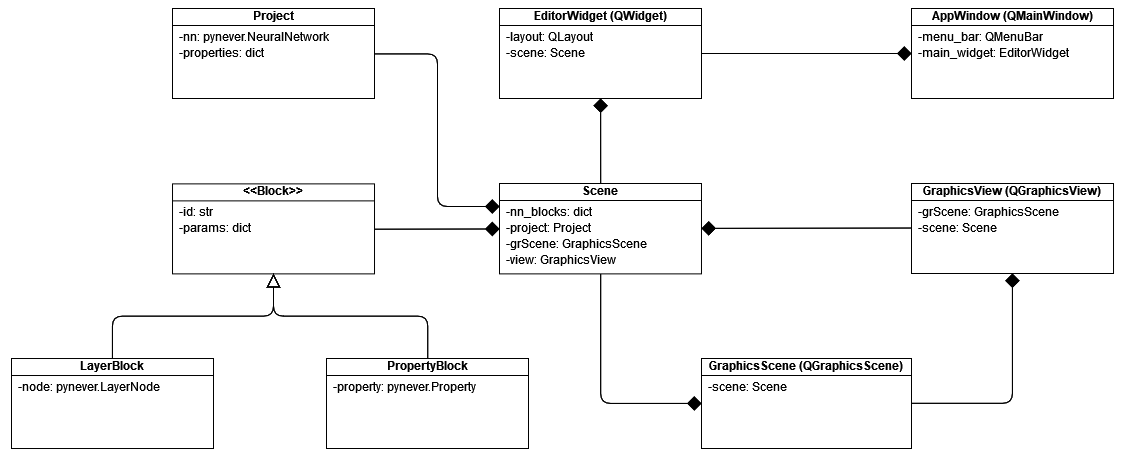
\includegraphics[width=\linewidth]{NN/CoCoNetCD.png}
\end{figure}

The architecture of \coconet{} is detailed in Figure~\ref{fig:cd_coconet}. Relying
on PyQt5's model for building GUIs, we use the classes \texttt{GraphicsScene} and
\texttt{GraphicsView} to control the logical model and the rendering, respectively.
In particular, we separate the building elements (blocks and edges) in the class
\texttt{Scene} from the methods and utilities for managing the exchange with the
view in \texttt{GraphicsScene}. The class \texttt{Project} serves as a
controller for reflecting the actions taken in the graphical environment to the
neural network that is built within \pynever. The main window of the application is 
displayed by the class \texttt{EditorWidget} which is associated with the 
\texttt{CoCoNetWindow} class containing the logic for displaying the 
\texttt{GraphicsView} and all the menus and layouts involved.

In order to comply with the VNN-LIB standard we have two kinds of available blocks:
the \texttt{LayerBlock} that represent the layers of a neural network, and the
\texttt{PropertyBlock} that represent a property to link to the input or the output
of the network. Each \texttt{LayerBlock} is initialized with a \texttt{LayerNode}
object from \pynever, i.e., represents a layer of the neural network displaying
all the fields and allowing the modification of some parameters. \texttt{PropertyBlock}
objects are initialized with a \pynever{} property, which allows to define a SMT-based
rule on the input and/or the output.

\subsection{Application interface}

\begin{figure}[t]
	\caption{\label{fig:coconet_gui} Screenshot of \coconet's GUI. The network
		is displayed in the Graphics Scene, and there is a toolbar with the 
		available blocks divided in nodes and properties on the left.}
	\centering
	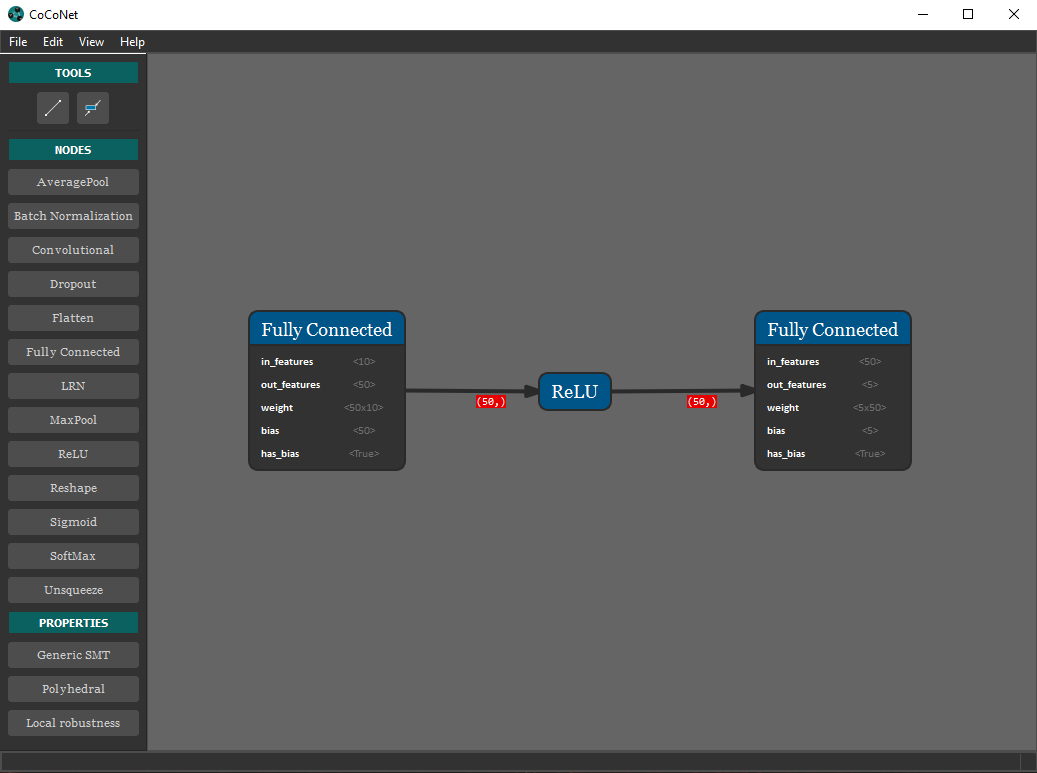
\includegraphics[width=.8\linewidth]{NN/CoCoNet_net.png}
\end{figure}

Figure~\ref{fig:coconet_gui} is a screenshot of \coconet's main window. The
view contains a simple network with a single Fully Connected layer with a ReLU
activation function. The available layers from \pynever{} are displayed in the
left toolbar, where the last three entries are different versions of a property.
The displayed nodes show the information related to the corresponding node: while
the ReLU layer has no parameters, the Fully Connected layer shows the inputs, the
outputs and the dimension of the weight and bias matrices. When a network is loaded
or created in the view, it is possible to add properties or save it in the VNN-LIB
format creating one ONNX file for the network and a SMT-LIB file for the property.

It is possible to connect one or more properties to the neural network displayed,
in the left toolbar we have three alternatives:
\begin{itemize}
	\item \textit{Generic SMT} - a simple text dialog where it is possible to directly
		write a property in plain SMT-LIB language
	\item \textit{Polyhedral} - a property that allows to set an upper or lower bound
		to each variable the property is connected to
	\item \textit{Local robustness} - a property that allows to specify a pair of
		input and output samples with an $\epsilon$-$\delta$ perturbation
\end{itemize}
%
\begin{figure}[t]
	\centering
	\caption{\label{fig:properties} Screenshot of the edit dialogs for three properties
		available in \coconet. From left to right, as described in the dialog label, 
		there is the \textit{Generic SMT} property, the \textit{Polyhedral} property 
		and the \textit{Local robustness} property.}
	\begin{subfigure}{.3\linewidth}
		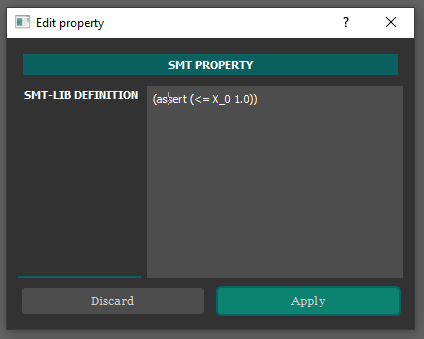
\includegraphics[width=\linewidth]{NN/Generic.png}
	\end{subfigure}
	\hspace*{\fill}
	\begin{subfigure}{.3\linewidth}
		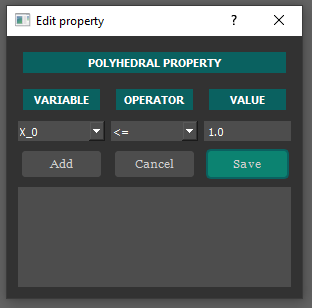
\includegraphics[width=\linewidth]{NN/Poly.png}
	\end{subfigure}
	\hspace*{\fill}
	\begin{subfigure}{.3\linewidth}
		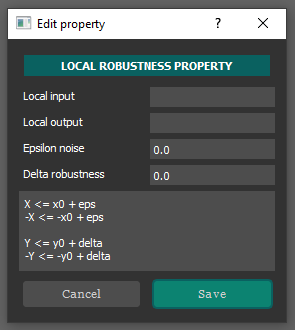
\includegraphics[width=\linewidth]{NN/LocRob.png}
	\end{subfigure}
\end{figure}
%
In Figure~\ref{fig:properties} we show the dialogs for the specification of the different
properties. For the \textit{Polyhedral} property the variables are constrained to the
number of inputs for a \textit{pre}-condition or the number of outputs for a 
\textit{post}-condition and can be bounded with all the relational operators, i.e.,
$<, \leq, =, >, \geq$. The \textit{Local robustness} property requires two samples, one
for the input and one for the output, and the two $\epsilon$ and $\delta$ measures.

Once the network and the properties are set, it is possible to save the benchmark in the
VNN-LIB format: using the \textit{Save as...} menu, it is possible to select 
\textit{VNN-LIB} as the output file format. In this way, the neural network will be saved
--- or converted, if opened as a different format --- as an ONNX file and the properties
will be stored in a separate SMT-LIB file with the same name of the network.
%\include{Chapter5/never2}

%\chapter{Experimental analysis}
%\label{ch:experiments_nn}
%\section{Case studies}
\label{sec:nn-exp_case}

Here we describe our case studies developed in order to experiment with
our algorithms and to build new benchmarks for the verification community:
Adaptive Cruise Control~\cite{DBLP:conf/ecms/DemarchiGPT22} and drone
control.
The purpose of creating a new benchmark for the evaluation of verification 
algorithms is that, while the verification community has been prolific in 
developing novel methodologies, very few general benchmarks have been proposed,
among which the most popular is still the ACAS XU 
benchmark~\cite{DBLP:conf/cav/KatzBDJK17}, released in 2017.

Furthermore, autonomous driving and drone control are tasks relevant for modern
applications and, at the same time, the neural networks used in this kind of 
control are usually small enough for the existing verification methodologies 
to be successfully applied. 

\subsection{Adaptive Cruise Control}

Technically, an adaptive cruise control (ACC) is an autonomous driving
function of level one\footnote{``Taxonomy and Definitions for Terms
	Related to Driving Automation Systems for On-Road Motor Vehicles'',
	SAE Standards, J3016\_202104.}, which controls the
acceleration of the \emph{ego car} --- the car whereon the ACC is
installed --- along the longitudinal axis. An ACC has two competing
objectives: keeping 
the ego car at the speed set by the user (\textit{speed following
	mode}) and keeping a safe distance from the \emph{exo car} in front
(\textit{car following mode}). The ACC that we consider has one
output, i.e., the acceleration $a$ suggested to the ego car in
$m \cdot s^{-2}$, and five inputs, two of which are fixed:
%
\begin{itemize}
	\item $v_p [m \cdot s^{-1}]$: the speed of the ego car.
	\item $v_r [m \cdot s^{-1}]$: the speed of the exo car relative to
	the ego car; when there is no exo car, this input has the value
	$0$.  
	\item $D [m]$: the actual distance between the ego car and the exo
	car; when there is no exo car or when the exo car is farther than
	$150m$ this input has the default value of $150m$.  
	\item $TH [s]$: Minimum headway time; this is the minimum
	time gap between the exo car and the ego car: $TH \cdot
	v_p$ corresponds to $D_s$, i.e.,the \emph{minimum safety
		distance}.
	\item $D_0 [m]$: A safety margin to be added to the minimum safety
	distance $D_s$.
\end{itemize}
%
In production vehicles the ACC function is implemented using classical
control laws. We view the production function --- called $ACC_{o}$
in the following --- as a black-box whose behavior should be learned
by a neural network.

\begin{figure}[t]
	\caption{Box plot for a million samples of the Adaptive Cruise Control 
		data set ($TH = 1.5$; $D_0 = 5$)}
	\label{fig:cruise-boxplot}
	\centering
	\scalebox{0.25}{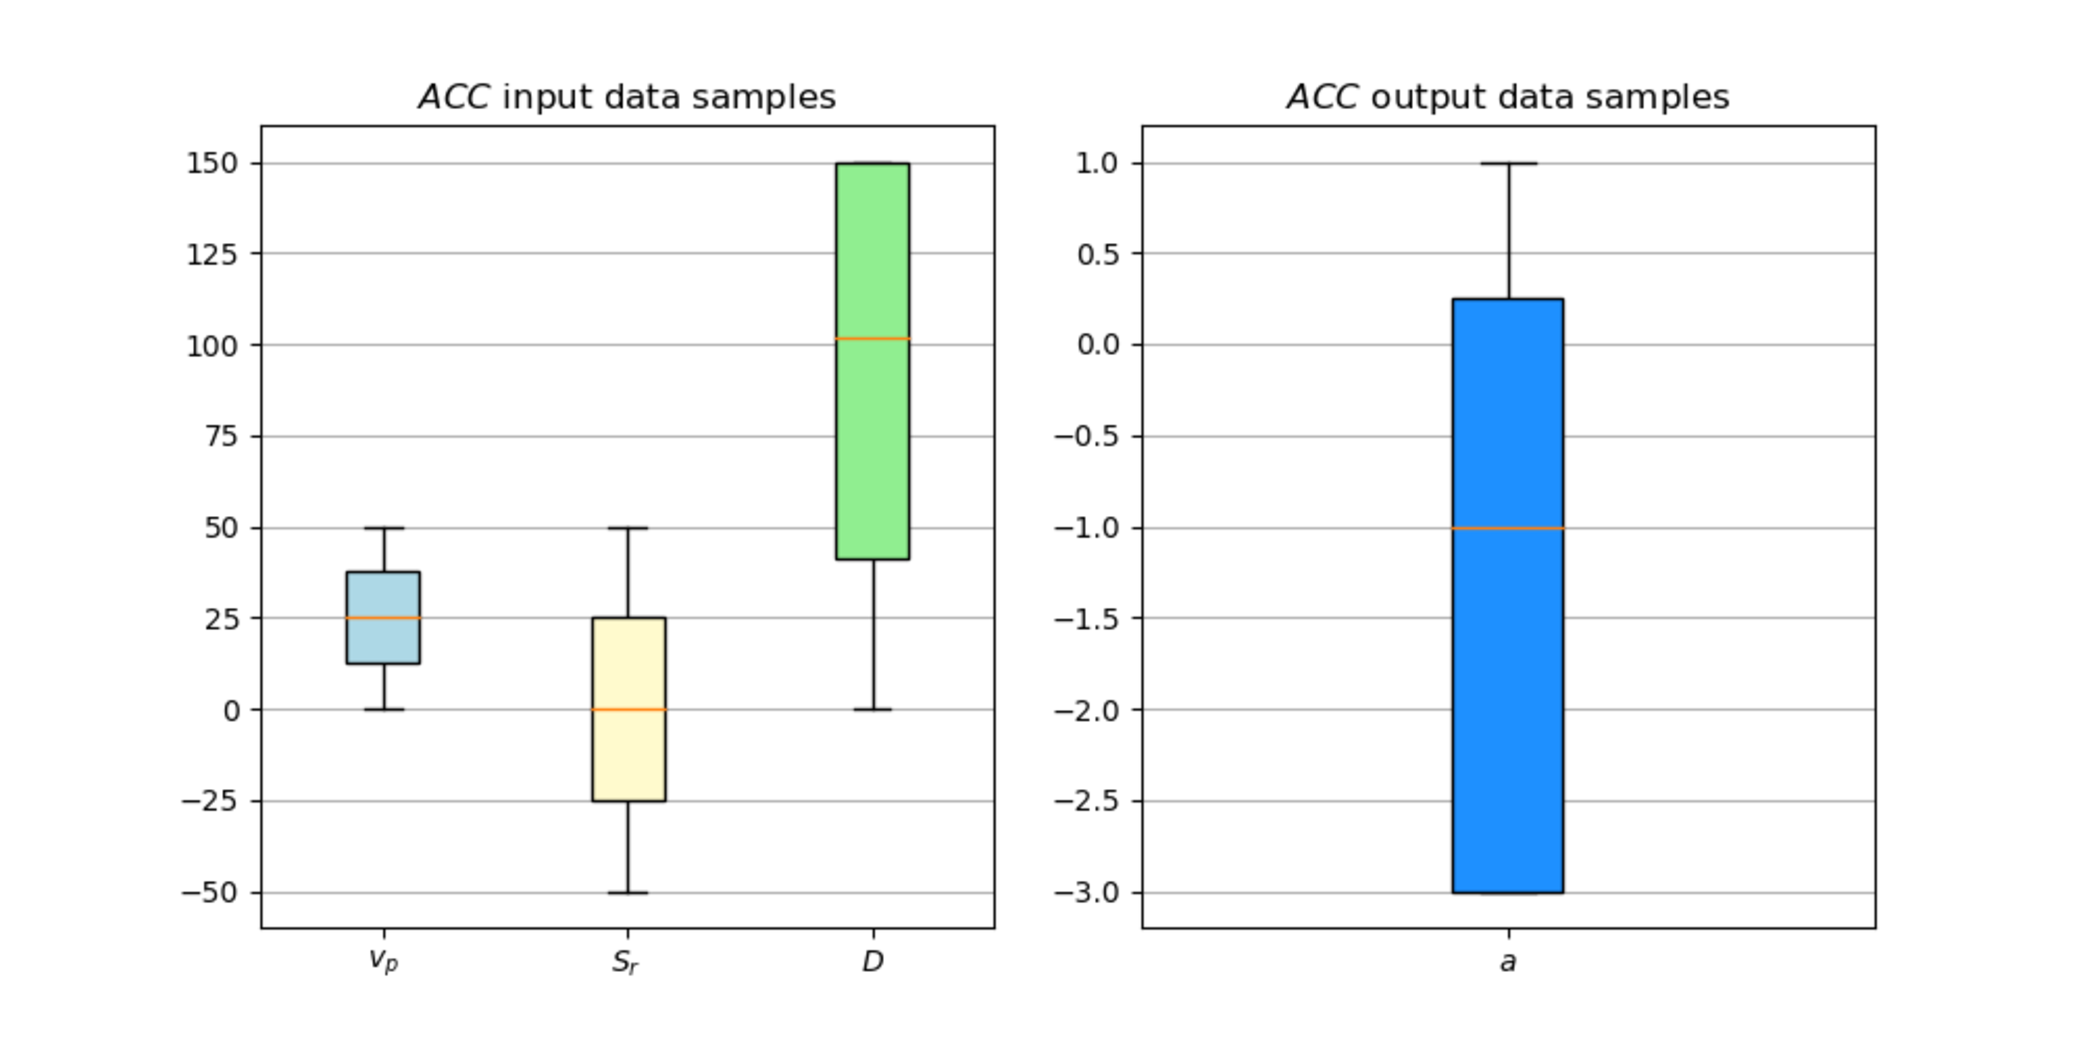
\includegraphics{NN/acc_samples.pdf}}
\end{figure}

Given the goal of learning $ACC_{o}$ using a NN, we should generate
several instances of input-output data using, e.g., a car
simulator. Since a simulator was unavailable to us at the time of this 
writing, we generated the dataset to learn various NNs by drawing
samples from uniform distributions over the input values of $ACC_{o}$,
considering the following lower and upper bounds for $v_p$, $v_r$ and $D$:
%
\begin{equation}
	\begin{aligned}
		0 & \leq v_p \leq 50 \\
		-50 & \leq v_r \leq 50 \\
		0 & \leq D \leq 150
	\end{aligned}
	\label{eq:outbounds-in}
\end{equation}
%
The values of $TH$ and $D_0$ are kept fixed, and we obtain the
corresponding output $a$ by feeding $ACC_{o}$ with the generated inputs. 
We generate 16 different data sets, each composed by a million
samples, that feature 16 different combinations of $TH$ and $D_0$,
where $TH \in \{1, 1.5, 2, 2.5\}$, while $D_0 = \{2.5, 5, 7.5, 10\}$. 
Figure \ref{fig:cruise-boxplot} shows the distributions of input and
output samples using box plots in the case $TH=1.5$ and $D_0 = 5$.

We tested three NN architectures comprised of affine and ReLU
layers: we refer to them as \textit{Net0}, \textit{Net1} and
\textit{Net2} in the following. These NNs feature increasing complexity 
both in terms of the number of layers and in the amount of neurons per 
layer. The networks considered differ from one another only for the details 
of the hidden layers, which are the following:
%
\begin{itemize}
	\item \textit{Net0}: two affine layers of 20 and 10 neurons respectively, 
	each followed by a ReLU layer;
	\item \textit{Net1}: two affine layers of 50 and 40 neurons respectively, 
	each followed by a ReLU layer;
	\item \textit{Net2}: four affine layers of 20, 20, 20 and 10 neurons 
	respectively, each followed by a ReLU layer.
\end{itemize}
%
The input of the network is in all the cases a three dimensional vector.
All the networks present an output layers consisting
of a linear layer of dimension 1 (without a following ReLU layer).

To learn the NNs we split the data sets in two parts,
one for training and one for testing, with the ratio of 4:1. Our
training phase lasts $100$ epochs for each of the $16$ data sets. We
consider the \textit{Adam} optimizer~\cite{kingma2017adam} and the
\textit{ReduceLROnPlateau} scheduler. For both our loss
function and our performance metric we leveraged the \textit{Mean
	Squared Error (MSE) loss}. We set batch sizes to $32$ for training,
validation, and test sets. In our setup, we dedicated $30\%$ of the
training set to the validation process. Concerning the optional
parameters, we also set the learning rate to $0.01$, the weight decay
to $0.0001$ and the training scheduler patience to $3$, i.e., the
number of consecutive epochs without loss decrease that triggers
training procedure abortion. All the training is perfomed inside
\nevertwo{} which, in turn, is based on the \textsc{pyTorch}
library. For this reason, all the remaining parameters required by 
learning algorithms are set to their default \textsc{pyTorch} values.

\paragraph{Verification setup.}
We consider three properties to be verified for the ACC case study, 
and we verify them in \nevertwo{} with different NNs. The first property 
that we define, called \textit{OutBounds} in the following, simply 
checks that the output acceleration does not exceed the bounds of the
$ACC_o$ function. Stated formally, this amounts to have \nevertwo{} check
that, given the preconditions in Eq. (\ref{eq:outbounds-in}) the output 
$a$ satisfies the postcondition
%
\begin{equation}
	-3 \leq a \leq 1.
	\label{eq:outbounds-out}
\end{equation}
%
The second property we consider is called \textit{Near0}, and it is
aimed at making sure that the ACC system does not output positive
accelerations when the vehicle ahead is too close. We frame this
concept via the precondition
%
\begin{equation}
	\begin{aligned}
		0 & \leq v_p \leq 50 \\
		-50 & \leq v_r \leq 50 \\
		0 & \leq D \leq 150\\
		TH \cdot v_r + D_0 & \geq D + \varepsilon
	\end{aligned}
	\label{eq:near0-in}
\end{equation}
%
where $\varepsilon \in {\mathbb{R}^+}$ is a positive tolerance
value in the last inequality. Notice that the input bounds are the
same as \textit{Outbound}. The last inequality 
stems from the fact that $TH \cdot v_r$ is the safety distance
required to stop the ego car in time if the exo car brakes, and
$D_0$ is a buffer value which, like $TH$, is constant for each data
set. The corresponding output postcondition for \textit{Near0} is
%
\begin{equation}
	-3 \leq a \leq 0.
	\label{eq:near0-out}
\end{equation}
%
Intuitively, we do not want the network to output positive
accelerations in this case.

Finally, the last property we consider is \textit{Far0}, which is
symmetrical with respect to \textit{Near0}. The precondition is
%
\begin{equation}
	\begin{aligned}
		0 & \leq v_p \leq 50 \\
		-50 & \leq v_r \leq 50 \\
		0 & \leq D \leq 150\\
		TH \cdot v_r + D_0 & \leq D - \varepsilon
	\end{aligned}
	\label{eq:far0-in}
\end{equation}
%
where $\varepsilon \in {\mathbb{R}^+}$ is still a tolerance value and the
input bounds coincide with \textit{OutBounds} and \textit{Near0}
properties. In this case, we want to verify that when the ego car
is too far from the exo car (or there is no vehicle ahead at all), the
NN does not suggests negative accelerations. The output postcondition is
%
\begin{equation}
	0 \leq a \leq 1.
	\label{eq:far0-out}
\end{equation}

In our experiments, we consider two different sub-settings for the mixed
algorithm, called \textit{mixed} and \textit{mixed2} which differ in the
number of neurons to refine, either $1$ or $2$, respectively.

\subsection{RL-based drone hovering}

\begin{figure}[t]
	\caption{\label{fig:drone}The Bitcraze Crazyflie 2.1 drone
		considered in our setup}
	\centering
	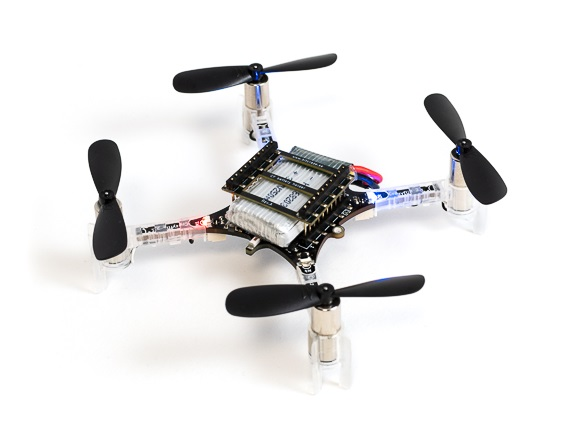
\includegraphics[width=.6\linewidth]{NN/drone_real.jpg}
\end{figure}
%
Here we consider another benchmark which is based on a reinforcement learning
environment: autonomous drone control. In particular, we consider the 
problem of making a drone take off and hover at a chosen altitude. Our motivation 
for dealing with a robotics framework is twofold: first, the control problems
arising in robotics are more and more relevant in the real world scenario; drones
and unmanned agents in general are being employed in several tasks that require
a high confidence in the agent. Second, using the Soft Actor-Critic architecture 
we are able to employ reasonable-sized network architectures for the agent that 
we are able to verify, and we delegate the more complex tasks to the critic which 
is not required to be certified.

We focused on building a modular setup for the generation of benchmarks using well-maintained
and stable resources to be able to easily extend it to new case studies and network 
architectures. In particular, we leveraged:
%
\begin{itemize}
	\item \gym\footnote{https://github.com/openai/gym}: an open source Python 
	library providing a standard API for communication between reinforcement 
	learning algorithms and environments.
	\item \stableb\footnote{https://github.com/DLR-RM/stable-baselines3}: an 
	open source training framework providing scripts for training and evaluating 
	RL agents using standard state-of-the-art algorithms.
	\item \pybullet\footnote{https://pybullet.org/}: an open source physics 
	simulator for robotics and reinforcement learning.
	\item \drones\footnote{https://github.com/utiasDSL/gym-pybullet-drones}: an 
	open source \gym-stile environment supporting the definition of various 
	learning tasks on the control of one or more quadcopters.
\end{itemize}
%
Using these open source resources we greatly simplified the complexity of our 
setup and we were able to directly train the network of interest in the environment 
corresponding to our case study with the chosen state-of-the-art RL algorithm.
In Figure~\ref{fig:drone} we show the quadcopter model of choice,
which was the default one proposed in \drones{} (Bitcraze's Crazyflie 2.x).
To evaluate our algorithms we built the experimental setup detailed in the following.
%
\paragraph{RL setup.} The reinforcement learning setup we used to train 
our model was based on the one proposed by~\cite{DBLP:conf/iros/PaneratiZZXPS21}: 
in particular, we leveraged their \textsc{HoverAviary} environment, together with 
the \stableb{} implementation of the Soft Actor-Critic (SAC) algorithm,
to train our neural networks of interest. We chose this algorithm because
it is more stable than traditional actor-critic algorithms, but it still makes
use of two different networks: the \textit{actor} to learn a
policy and the \textit{critic} to approximate the optimal value
function. Because of this, it is possible to learn a relatively small
actor network, which is then subject to verification, while the critic
network can be as complex as the task requires without impacting on
the verification performances since only the actor network is relevant
for this purpose. 
The hyperparameters chosen for the SAC algorithm were the default ones proposed 
by \stableb{} except for the network architectures of the actor and the critic: 
in particular, for the critic we chose a fixed architecture with four hidden layers 
with $512, 256, 128, 64$ neurons, respectively, each followed by a ReLU layer, 
whereas for the actor we considered the eight different architectures presented in
Table~\ref{tab:ac-arch}.
%
\begin{table}[t]
	\caption{\label{tab:ac-arch}Actor network architectures used in our 
		experimental evaluation, arranged in two (\textit{AC1} to \textit{AC4}) 
		or three (\textit{AC5} to \textit{AC8}) hidden layers. The size of layers, 
		i.e., the number of neurons in each layer, is detailed in column 
		\textbf{No. of neurons}. Each hidden layer is followed by a ReLU layer.}
	\setlength{\tabcolsep}{15.5pt}
	\centering
	%\begin{tabular}{c c c}
	\begin{tabular}{l c r}
		\toprule
		\textbf{Architecture} & \textbf{Network ID} & \textbf{No. of neurons} \\
		\midrule
		\multirow{4}{*}{\textbf{Two layers}} & \textit{AC1} & 32, 16 \\
		& \textit{AC2} & 64, 32 \\
		& \textit{AC3} & 128, 64 \\
		& \textit{AC4} & 256, 128 \\
		\midrule
		\multirow{4}{*}{\textbf{Three layers}} & \textit{AC5} & 32, 16, 8 \\
		& \textit{AC6} & 64, 32, 16 \\
		& \textit{AC7} & 128, 64, 32 \\
		& \textit{AC8} & 256, 128, 64 \\
		\bottomrule
		\bigskip
	\end{tabular}
\end{table}

The observation type considered was the kinematic information (pose, linear and angular 
velocities) of the quadcopter, and the action type was the revolutions per minute 
(RPMs) applied to all the four rotors of the drone (similarly to what is done in
the experimental evaluation of~\cite{DBLP:conf/iros/PaneratiZZXPS21}).
All the actor models considered in our experiment were trained 
for 50000 steps and, at the end of the training process, the version
of the actor model 
presenting the best mean reward in an evaluation environment was chosen.
%
%
\paragraph{Verification setup.} The verification task we consider in our 
experiments is an analysis of the local robustness of our actor model with respect to 
small variations of the input, which could be interpreted as small noise on the 
sensors providing the input signal. Formally we consider the following assumption:
%
\begin{equation}
	\forall \varepsilon, x_0: \quad |x - x_0|_\infty \leq \varepsilon \quad \rightarrow \quad \nu(x_0) - \delta \leq \nu(x) \leq \nu(x_0) + \delta
	\label{eq:local-robustness}
\end{equation}
%
where $x_0$ is a specific input vector for the network $\nu$, and $\varepsilon$ and 
$\delta$ are scalar values representing the maximum noise on the input and the 
corresponding maximum output deviation, respectively. Our aim is to determine the 
values of $\delta$ corresponding to fixed values of $\varepsilon$ and $x_0$ for all 
the actors presented in Table~\ref{tab:ac-arch}.
The encoding of this verification task is straightforward in \nevertwo{}: we only need 
to define as input star the convex polytope defined by the constraints corresponding 
to $|x - x_0|_\infty \leq \varepsilon$ and then propagate it in our abstract network, 
applying the abstract transformer presented in Section~\ref{sec:relu_abst}, to 
obtain the abstract output set, whose stars can be easily analyzed to compute the 
reachable bounds of the output and, as a direct consequence, the maximum value of 
$\delta$. In the experiments we evaluated our complete, over-approximate and mixed 
algorithms: in particular, in our mixed algorithm we considered the case in which 
a single neuron is refined for each ReLU layer. We also considered two different 
values ($0.1$, $0.01$) for $\varepsilon$.
\\\\
Our experimental setup is available online in the public repository of
\pynever\footnote{https://github.com/NeVerTools/pyNeVer/tree/main/examples/submissions/IEEEAccess2023}, 
and the experiments herewith presented can be easily replicated.
The experiments were run on a machine with 2 Intel Xeon Gold 6432 CPUs and 128 GB of DDR4 RAM.
%
%\section{Experimental results}
\label{sec:nn-exp_results}

In this Section we present the evaluation of our methodology on the case studies
detailed before, as well as further experiments involving the star elimination
algorithm and the CEGAR algorithm presented in Sections~\ref{sec:optim} and
\ref{sec:cegar}.

\subsection{ACC}

\begin{table}[t!]
	\caption{\label{tab:acc_results} \nevertwo{} results for the ACC data set with
		$TH=1.5$ and $D_0=5$, with $\varepsilon = 0$ (left) and $\varepsilon = 20$
		(right). CPU time is in seconds rounded to the third decimal
		place. The best setting for each network and property is highlighted in 
		boldface.}
	\setlength{\tabcolsep}{9pt}
	\renewcommand{\arraystretch}{0.8}
	\centering
	%
	\begin{tabular}{c c c rr rr}
		\toprule
		\multirow{2}{*}{\textbf{Network ID}} & \multirow{2}{*}{\textbf{Property}} & 
		\multirow{2}{*}{\textbf{Setting}} & \multicolumn{2}{c}{$\varepsilon = 0$} &
		\multicolumn{2}{c}{$\varepsilon = 20$} \\
		\cmidrule{4-7}
		 & & & Result & Time & Result & Time \\
		\midrule
		%
		\multirow{12}{*}{\textit{Net0}} & \multirow{4}{*}{\textit{OutBounds}} 
		   & Over-approx & True & 5.139 & True & 5.037 \\
		 & & Mixed & True & \textbf{5.055} & True & 5.063 \\
		 & & Mixed2 & True & 5.112 & True & \textbf{4.996} \\
		 & & Complete & True & 6.273 & True & 6.203 \\
		 \cmidrule{2-7}
		 & \multirow{4}{*}{\textit{Near0}} 
		   & Over-approx & False & 5.666 & False & 5.034 \\
		 & & Mixed & False & 5.251 & False & 5.101 \\
		 & & Mixed2 & False & \textbf{5.203} & False & \textbf{4.965} \\
		 & & Complete & False & 6.319 & False & 5.345 \\
		 \cmidrule{2-7}
		 & \multirow{4}{*}{\textit{Far0}}
		   & Over-approx & False & 5.078 & False & 5.008 \\
		 & & Mixed & False & \textbf{4.986} & \textbf{True} & \textbf{5.016} \\
		 & & Mixed2 & False & 5.139 & True & 5.068 \\
		 & & Complete & False & 5.186 & True & 5.62 \\
		\midrule
		%
		\multirow{12}{*}{\textit{Net1}} & \multirow{4}{*}{\textit{OutBounds}}
		   & Over-approx & True & \textbf{5.931} & True & \textbf{5.948} \\
		 & & Mixed & True & 6.662 & True & 6.934 \\
		 & & Mixed2 & True & 7.309 & True & 7.232 \\
		 & & Complete & True & 51.683 & True & 52.318 \\
		 \cmidrule{2-7}
		 & \multirow{4}{*}{\textit{Near0}}
		   & Over-approx & False & \textbf{5.906} & False & \textbf{5.436} \\
		 & & Mixed & False & 6.676 & False & 5.797 \\
		 & & Mixed2 & False & 8.071 & False & 5.955 \\
		 & & Complete & False & 50.469 & False & 7.667 \\
		 \cmidrule{2-7}
		   & \multirow{4}{*}{\textit{Far0}} 
		 & Over-approx & False & \textbf{5.709} & False & \textbf{5.344} \\
		 & & Mixed & False & 5.888 & False & 5.776 \\
		 & & Mixed2 & False & 6.301 & False & 6.226 \\
		 & & Complete & False & 13.041 & False & 8.212 \\
		\midrule
		%
		\multirow{12}{*}{\textit{Net2}} & \multirow{4}{*}{\textit{OutBounds}}
		   & Over-approx & True & \textbf{9.525} & True & \textbf{9.532} \\
		 & & Mixed & True & 10.482 & True & 10.149 \\
		 & & Mixed2 & True & 12.525 & True & 12.065 \\
		 & & Complete & True & 26.958 & True & 26.794 \\
		 \cmidrule{2-7}
		 & \multirow{4}{*}{\textit{Near0}}
		   & Over-approx & False & \textbf{9.515} & False & 9.379 \\
		 & & Mixed & False & 10.292 & False & 9.872 \\
		 & & Mixed2 & False & 13.636 & False & 11.653 \\
		 & & Complete & False & 24.496 & \textbf{True} & \textbf{10.696} \\
		 \cmidrule{2-7}
		 & \multirow{4}{*}{\textit{Far0}}
		 & Over-approx & False & \textbf{9.753} & False & \textbf{9.453} \\
		 & & Mixed & False & 9.944 & False & 9.848 \\
		 & & Mixed2 & False & 12.148 & False & 11.558 \\
		 & & Complete & False & 13.27 & False & 10.854 \\
		\bottomrule
	\end{tabular}
\end{table}

We run our tests on a workstation featuring two
Intel Xeon Gold 6234 CPU, three NVIDIA Quadro RTX 6000/8000 GPUs (with
CUDA enabled), and 125.6 GiB of RAM running Ubuntu 20.04.03 LTS. For
the sake of brevity, we are only going to report here in 
Table~\ref{tab:acc_results} a fraction of the experiments we ran for 
the data set with $TH = 1.5$ and $D_0 = 5$, considering 
$\varepsilon = 0$ and $\varepsilon = 20$. The results we show here are 
consistent with the results obtained on other data sets that we do not 
report. In particular, looking at Table~\ref{tab:acc_results} we can 
observe that:
%
\begin{itemize}
	\item All the properties can be checked on all the networks in
		reasonable time by \nevertwo: less than one minute of CPU time is
		required independently from the network architecture and the
		specific setting considered.
	\item The complete setting is the most expensive in computational
		terms; given the considerations above this should come at no
		surprise, but in one case, namely \textit{Net2} on property
	\textit{Near0}, the complete setting is able to prevail over the 
		others, i.e., it certifies that the property is true; indeed mixed and
		over-approximated settings (shortened as over-approx in
		Table~\ref{tab:acc_results}) take less time, but state that the
		property is false because they do not manage to reach enough
		precision to state the correct result.
	\item The over-approximated setting is often faster than the other
		ones: 6 out of 9 cases for $\varepsilon = 0$ and 7 out of 9
		cases for $\varepsilon = 20$; however it must be noted that its
		results are definitive only when the property is true: 3 out of 9
		cases for both values of $\varepsilon$ and always for the (simplest)
		property \textit{OutBounds}.
	\item The mixed setting is at times faster than the
		over-approximated one, but only in one case, namely property
	\textit{Far0} on \textit{Net0} it is able to provide a definite
		answer while outperforming both the complete and over-approximated
		settings. 
\end{itemize}
%
Overall we can conclude that while further research is needed to improve 
on the capability of \nevertwo{} to provide definite answers with
faster techniques involving over-approximation, still the tool is able
to check a number of interesting properties in networks involving
hundreds of neurons in a relatively small amount of CPU time. We view
this as a positive result and an enabler for preliminary testing of
\nevertwo{} at industrial settings featuring networks of comparable size
to our ACC case study.

\subsection{Drones}
%
\begin{table}[t]
	\caption{\label{tab:exp-res}\nevertwo{} results for the drones case study.
		Column \textbf{Network ID} refers to the same actor architectures as
		detailed in Table~\ref{tab:ac-arch}. Column \textbf{Return} reports the 
		best return obtained during the testing of the Actors in the evaluation
		environment, while column \textbf{Epsilon} reports the $\varepsilon$ 
		values tested in our experiments. Columns \textit{\textbf{Over-approx}}, 
		\textit{\textbf{Mixed}} and \textit{\textbf{Complete}} refer to the 
		selected verification algorithm, with the maximum \textit{Delta} 
		($\delta$) obtained and the elapsed \textit{Time} in seconds, respectively. 
		The cells reporting ``--'' correspond to experiments in which our algorithm 
		was not able to complete the verification successfully in less than 
		70 seconds.}
	\setlength{\tabcolsep}{9pt}
	\centering
	%
	\begin{tabular}{c c c rr rr rr}
		\toprule
		\multirow{2}{*}{\textbf{Network ID}} & 
		\multirow{2}{*}{\textbf{Return}} & 
		\multirow{2}{*}{\textbf{$\varepsilon$}} & 
		%\multicolumn{6}{c}{\textbf{Algorithm}} \\
		% & & & 
		\multicolumn{2}{c}{\textbf{\textit{Over-approx}}} &
		\multicolumn{2}{c}{\textbf{\textit{Mixed}}} &
		\multicolumn{2}{c}{\textbf{\textit{Complete}}} \\
		\cmidrule{4-9}
		& & & $\delta$ & Time & $\delta$ & Time & $\delta$ & Time \\
		%
		\midrule
		%
		\multirow{2}{*}{\textit{AC1}} & \multirow{2}{*}{-27.15} &
		0.10 & 4.18 & 0.48 & 3.71 & 0.51 & 3.23 & 0.61 \\
		& & 0.01 & 0.34 & 0.47 & 0.33 & 0.49 & 0.33 & 0.47 \\
		% 
		\multirow{2}{*}{\textit{AC2}} & \multirow{2}{*}{-27.28} &
		0.10 & 2.40 & 0.71 & 2.11 & 0.78 & 1.82 & 5.91 \\
		& & 0.01 & 0.10 & 0.52 & 0.10 & 0.52 & 0.10 & 0.58 \\
		%
		\multirow{2}{*}{\textit{AC3}} & \multirow{2}{*}{-27.33} &
		0.10 & 12.90 & 2.66 & 12.86 & 2.82 & -- & -- \\
		& & 0.01 & 1.51 & 0.79 & 1.51 & 0.76 & 1.51 & 1.08 \\
		%
		\multirow{2}{*}{\textit{AC4}} & \multirow{2}{*}{-27.69} &
		0.10 & 6.23 & 5.37 & 5.91 & 8.60 & -- & -- \\
		& & 0.01 & 0.41 & 1.27 & 0.40 & 1.58 & 0.40 & 11.84 \\
		%
		\multirow{2}{*}{\textit{AC5}} & \multirow{2}{*}{-28.31} &
		0.10 & 17.65 & 0.82 & 17.09 & 0.83 & 14.40 & 2.25 \\
		& & 0.01 & 1.20 & 0.73 & 1.20 & 0.74 & 1.20 & 0.76 \\
		%
		\multirow{2}{*}{\textit{AC6}} & \multirow{2}{*}{-27.63} &
		0.10 & 1.99 & 0.94 & 1.79 & 0.98 & 1.57 & 7.79 \\
		& & 0.01 & 0.11 & 0.77 & 0.11 & 0.78 & 0.11 & 0.78 \\
		%
		\multirow{2}{*}{\textit{AC7}} & \multirow{2}{*}{-32.06} &
		0.10 & 2.89 & 1.84 & 2.45 & 2.02 & 2.24 & 61.81 \\
		& & 0.01 & 0.23 & 0.95 & 0.23 & 0.99 & 0.23 & 1.18 \\
		%
		\multirow{2}{*}{\textit{AC8}} & \multirow{2}{*}{-27.81} &
		0.10 & 30.14 & 9.50 & 28.97 & 14.45 & -- & -- \\
		& & 0.01 & 0.56 & 1.63 & 0.56 & 1.78 & 0.56 & 4.91 \\
		\bottomrule
		\bigskip
	\end{tabular}
\end{table}
%
From the results reported in Table~\ref{tab:exp-res} it would seem that, 
at least for the task considered, an increased size for the actor network does 
not necessarily correspond to an increase in performance. This would seem to 
support our belief that, in this kind of control task, small networks yield 
adequate performances, and therefore are still relevant in meaningful applications. 
Furthermore, from the values of $\delta$ obtained by our reachability analysis, 
it would seem that bigger networks do not present significantly increased 
robustness to local perturbation and, at least in our experiments, they often 
result to be less robust than smaller ones.
Regarding the comparison between the different reachability algorithms we notice 
that, as expected, the values of $\delta$ found by the complete algorithm are 
stricter than --- or as strict as --- the ones found by the mixed algorithm, and 
that the same behavior can be observed between the mixed and over-approximate 
algorithms. As we would expect, the computational time needed by the different 
algorithms increases with their complexity and the only exceptions appear to be
when the coarser algorithms are already good enough to compute a very strict 
$\delta$, which means that the number of unstable ReLU --- causing the loss of 
precision and the splitting of the stars in the over-approximate and complete 
algorithm respectively --- is extremely limited.

\subsection{Star elimination}

\begin{table}[t!]
	\setlength{\tabcolsep}{13pt}
	\centering
	\caption{\label{tab:acas_optim} Experimental results for the star elimination 
		algorithm on the ACAS Xu benchmark. The number of stars layer-by-layer for
		each network is compared between the original algorithm and the 
		elimination-based version. All times are expressed in seconds.}
	\begin{tabular}{c c rr rr}
		\toprule
		\multirow{2}{*}{\textbf{Network ID}} & \multirow{2}{*}{\textbf{Layer}} & 
		\multicolumn{2}{c}{\textbf{Original}} & \multicolumn{2}{c}{\textbf{Elimination}} \\
		\cmidrule{3-6} 
		 & & No. of stars & Time & No. of stars & Time \\
		\midrule
 		\multirow{6}{*}{\textit{1\_1}}
 		 & 1 & 18 & 10.89 & 18 & 10.9 \\ 
 		 & 2 & 49 & 11.36 & 49 & 11.48 \\ 
 		 & 3 & 230 & 12.43 & 230 & 12.56 \\ 
 		 & 4 & 1466 & 24.42 & 1465 & 24.52 \\ 
 		 & 5 & 3894 & 67.02 & 3864 & 66.19 \\ 
 		 & 6 & 31706 & 305 & 31025 & 303.72 \\ 
 		  & & & & & \\
 		\multirow{6}{*}{\textit{1\_3}}
 		 & 1 & 2 & 10.8 & 2 & 10.72 \\ 
 		 & 2 & 30 & 11.27 & 30 & 11.04 \\ 
 		 & 3 & 146 & 12.21 & 146 & 12.48 \\ 
 		 & 4 & 287 & 13.75 & 287 & 13.87 \\ 
 		 & 5 & 1700 & 28.52 & 1686 & 28.58 \\ 
 		 & 6 & 4121 & 69.78 & 4066 & 70.36 \\ 
 		  & & & & & \\
 		\multirow{6}{*}{\textit{2\_3}}
 		 & 1 & 11 & 10.75 & 11 & 11.04 \\ 
 		 & 2 & 35 & 10.95 & 35 & 11.15 \\ 
 		 & 3 & 102 & 11.77 & 102 & 12 \\ 
 		 & 4 & 230 & 13.31 & 230 & 13.59 \\ 
 		 & 5 & 408 & 17.46 & 408 & 17.26 \\ 
 		 & 6 & 2128 & 30.58 & 2115 & 30.75 \\ 
 		\bottomrule
	\end{tabular} 
\end{table}

Here we show some preliminary results on the star elimination algorithm detailed in
Section~\ref{sec:optim}. For the comparison, we considered three networks from the 
ACAS Xu evaluation~\cite{DBLP:conf/cav/KatzBDJK17} and the networks for drone control
presented before. ACAS Xu is an airborne collision avoidance system based on DNNs 
whose purpose is to issue advisory commands to an autonomous vehicle (ownship) about
evasive maneuvers to be performed if another vehicle (intruder) comes too close. 
In particular, we selected Property 3 and 4 since they could be easily expressed as
a single verification query in our tool.
In the words of~\cite{DBLP:conf/cav/KatzBDJK17}, these safety properties 
``\textit{deal with situations where the intruder is directly ahead of the ownship 
	and state that the NN will never issue a COC (clear of conflict) advisory}''.
Considering the analysis in~\cite{DBLP:conf/cav/KatzBDJK17}, each property can be
assessed on 42 different networks depending on the choice of two parameters, i.e.,
the the previous advisory value and the time to loss of vertical separation.

\begin{table}[t!]
	\setlength{\tabcolsep}{9pt}
	\centering
	\caption{\label{tab:rcra_optim} Experimental results for the star elimination 
		algorithm on the drone case study, both with $\varepsilon = 0.01$ and 
		$\varepsilon = 0.1$. The number of stars layer-by-layer for each network is
		compared between the original algorithm and the elimination-based version.
		All times are expressed in seconds.}
		\resizebox{\columnwidth}{!}{%
		\begin{tabular}{c c rr rr rr rr}
			\toprule
			\multirow{3}{*}{\textbf{Network ID}} & \multirow{3}{*}{\textbf{Layer}} & 
			\multicolumn{4}{c}{$\varepsilon = 0.01$} & \multicolumn{4}{c}{$\varepsilon = 0.1$} \\
			\cmidrule{3-10}
			&  & \multicolumn{2}{c}{Original} & \multicolumn{2}{c}{Elimination} &
			\multicolumn{2}{c}{Original} & \multicolumn{2}{c}{Elimination} \\
			&  & Stars & Time & No. of stars & Time & No. of stars & Time & No. of stars & Time \\
			\midrule
			\multirow{2}{*}{\textit{AC1}}
			& 1 & 17 & 11.67 & 17 & 11.35 & 520 & 16.67 & 518 & 17.13 \\ 
			& 2 & 25 & 11.34 & 25 & 11.33 & 2660 & 22.84 & 2579 & 25.01 \\ 
			& & & & & & & & & \\
			\multirow{2}{*}{\textit{AC2}}
			& 1 & 3 & 11.13 & 1 & 11.23 & 3187 & 56.21 & 2712 & 72.09 \\ 
			& 2 & 5 & 11.15 & 1 & 11.09 & 6397 & 119.24 & 5367 & 103.82 \\
			& & & & & & & & & \\
			\multirow{2}{*}{\textit{AC3}}
			& 1 & 18 & 11.90 & 5 & 11.63 & - & - & 5008 & 228.73 \\ 
			& 2 & 81 & 12.77 & 14 & 11.43 & - & - & - & - \\ 
			& & & & & & & & & \\
			\multirow{2}{*}{\textit{AC4}}
			& 1 & 226 & 24.54 & 226 & 24.70 & - & - & - & - \\ 
			& 2 & 490 & 39.52 & 487 & 43.48 & - & - & - & - \\
			& & & & & & & & & \\
			\multirow{3}{*}{\textit{AC5}}
			& 1 & 3 & 11.03 & 3 & 11.06 & 1962 & 20.24 & 966 & 19.34 \\ 
			& 2 & 5 & 11.08 & 5 & 11.10 & 4677 & 42.71 & 1993 & 25.29 \\ 
			& 3 & 5 & 11.00 & 5 & 11.10 & 11318 & 49.97 & 4572 & 27.07 \\ 
			& & & & & & & & & \\
			\multirow{3}{*}{\textit{AC6}}
			& 1 & 4 & 11.08 & 4 & 11.21 & 5992 & 105.60 & 3504 & 94.00 \\ 
			& 2 & 4 & 11.06 & 4 & 11.15 & 11593 & 198.89 & 6287 & 128.23 \\ 
			& 3 & 4 & 11.11 & 4 & 11.03 & - & - & 14298 & 171.42 \\ 
			& & & & & & & & & \\
			\multirow{3}{*}{\textit{AC7}}
			& 1 & 16 & 11.32 & 16 & 11.38 & - & - & - & - \\ 
			& 2 & 43 & 11.87 & 43 & 11.92 & - & - & - & - \\ 
			& 3 & 88 & 12.14 & 87 & 12.03 & - & - & - & - \\ 
			& & & & & & & & & \\
			\multirow{3}{*}{\textit{AC8}}
			& 1 & 12 & 12.30 & 10 & 12.94 & - & - & - & - \\ 
			& 2 & 18 & 12.41 & 14 & 12.07 & - & - & - & - \\ 
			& 3 & 45 & 11.89 & 30 & 11.62 & - & - & - & - \\ 
			\bottomrule 
	\end{tabular}}
\end{table}

Table~\ref{tab:acas_optim} shows the results of the elimination algorithm for three
networks in the ACAS Xu set. We selected only three networks as they are representative
enough for the analysis herewith presented. Column ``\textbf{Layer}'' refers to the
layer of the network in which we analyize the abstract propagation: each network in the
ACAS Xu pool is made of six layers and in each layer the number of stars increases.
Comparing the original algorithm and the optimized one, we can see that in this case
the number of stars that can be deleted is almost neglectable: in network \textit{1\_1}
we remove less than 700 stars in the last layer, with more than 31k stars alone.
On the other hand, the comparison of CPU time is encouraging: even with the overhead
introduced by Algorithm~\ref{alg:prop_v2} we do not pay a significant toll. This
allows us to determine that, at least, we can always try in principle to optimize the
number of stars in the propagation.

In Table~\ref{tab:rcra_optim} we show a more encouraging result. We applied the same
elimination algorithm to the drones case study and in this case the experiments
show that star elimination can actually improve the performance of the verification
algorithm. Comparing the results with $\varepsilon = 0.01$ and $\varepsilon = 0.1$ we
observe that in the former case we propagate a very small number of stars: this is
reasonable since a tighter input bound is more likely to be more stable. This 
stability makes the elimination-based version very similar to the original one 
with notable exceptions, e.g., in network \textit{AC2} all the extra stars created 
in the original algorithm can be deleted and only one star is significative. 
The experiment with $\varepsilon = 0.1$ is more representative since the number of 
stars grows higher. Here we obtain slightly better results than ACAS Xu for networks 
\textit{AC1} and \textit{AC2}, but already in \textit{AC3} the optimized algorithm 
manages to propagate the first layer within a timeout of 5 minutes where the original 
algorithm fails. Then, on networks \textit{AC5} and \textit{AC6} it manages to cut 
the number of stars in less than a half with a valuable speed-up in computational time, 
too.

Given the preliminary nature of these experiments, the discrepancy between the CPU
times in Tables~\ref{tab:exp-res} and~\ref{tab:rcra_optim} is due to the fact that
the latter experiments are run on a machine equipped with an Intel\textregistered  
\hspace{1pt} Core\texttrademark \hspace{1pt} i7-6500U dual core CPU @ 2.50GHz, 
featuring 8GB of RAM and running Ubuntu Linux 16.04 LTS 64 bit.

\subsection{CEGAR}
%
\begin{table}[t]
	\caption{\label{tab:ref_results} Experimental results for CEGAR on a subset of 
		ACAS Xu networks. Columns \textbf{Property} and \textbf{Network ID} report 
		the property and the network considered, respectively. The other columns 
		report the verification time in seconds and result (\textit{Verified}) 
		for \textbf{Mixed}, \textbf{CEGAR-PS} and \textbf{CEGAR-mR} analyses, 
		respectively. Given the randomic nature of the counter-example generator,
		we report the average time and the number of results over 10 repetitions 
		of the experiment.}
	\setlength{\tabcolsep}{9pt}
	\centering
	%
	\resizebox{\columnwidth}{!}{%
	\begin{tabular}{l l rr rr rr}
		\toprule
		\multirow{2}{*}{\textbf{Property}} & \multirow{2}{*}{\textbf{Network ID}} &
		\multicolumn{2}{c}{\textbf{Mixed}} & 
		\multicolumn{2}{c}{\textbf{CEGAR-PS}} &
		\multicolumn{2}{c}{\textbf{CEGAR-mR}} \\ 
		\cmidrule{3-8} 
		 & & Time & Verified & Time & Verified & Time & Verified \\ 
		\midrule
		\multirow{5}{*}{\textit{\# 3}} 
		& \textit{1\_1} & 13 & True & 10 & 3/10  & 9 & 9/10  \\ 
		& \textit{1\_3} & 10 & True & 14 & 6/10 & 10 & 0/10  \\ 
		& \textit{2\_3} & 7 & True & 10 & 9/10  & 7 & 6/10  \\ 
		& \textit{4\_3} & 15 & True & 17 & 10/10 & 14 & 10/10 \\ 
		& \textit{5\_1} & 6 & True & 11 & 10/10 & 9 & 10/10 \\
		 & & & & & & & \\
		\multirow{4}{*}{\textit{\# 4}}
		& \textit{1\_1} & 11 & True & 10 & 0/10  & 9 & 0/10 \\ 
		& \textit{1\_3} & 8 & True & 16 & 0/10  & 11 & 0/10  \\ 
		& \textit{3\_2} & 12 & True & 12 & 10/10 & 12 & 10/10 \\ 
		& \textit{4\_2} & 12 & True & 11 & 10/10 & 12 & 10/10 \\
		\bottomrule
	\end{tabular}}
\end{table}
%
Here we provide the results of the empirical evaluation of the CEGAR method.
All the	experiments ran on a laptop equipped with an Intel i7-8565 CPU 
(8 core at 1.8GHz) and 16 GB of memory with Ubuntu 20 operating system.
We test the CEGAR algorithm on the ACAS Xu benchmark: among the networks 
available, we selected those for which our over-approximate
analysis could not find a  definitive answer, ending with a total of 9 networks. 
 
In Table~\ref{tab:ref_results} we show the performance of the two versions of the
refinement algorithm explained in Section~\ref{sec:cegar}, and we compare them 
with our mixed abstraction methodology. The PS refinement (\textit{CEGAR-PS}) 
selects six neurons in the whole network to refine, while the mR refinement 
(\textit{CEGAR-mR}) refines one single neuron for each layer.
Note that, by design, the number of neurons refined is the same for every 
methodology: six in the whole network. The difference between the three algorithms 
is which neurons are selected and how. As can be seen, the performances of the 
two refinement algorithms are comparable; however, they seem to be less effective 
than our mixed methodology and CEGAR-PS seems to be slightly more accurate than 
CEGAR-mR at the cost of a small increase in the time needed to solve the query.
We believe that the difference in performance is mainly attributable to the fact 
that, while the measurements of relevance we used are valid, they do not capture how 
the coarseness of the abstraction changes dynamically when a particular neuron is 
refined. On the contrary, the mixed methodology chooses in each layer the neuron to 
refine based on the values of the areas of the triangles given the previous layer 
output. As a consequence, the choice of which neurons to refine is guided by the 
coarseness of the abstraction \emph{after} the refinement is already applied in the 
previous layers.

%*******************************************************************************
%******************************** CONCLUSIONS **********************************
%*******************************************************************************
%\chapter{Conclusions and Future work}
%\label{ch:conclusions}
%\section{Conclusions}
\label{sec:concl}
%
The work presented in this Thesis has advanced the state of the art with the
following contributions:
%
\begin{itemize}
	\item We experimented with declarative encodings for the automated design
		of a complex system, and generalized some best practices that can
		apply to different case studies.
	\item We expanded and structured the reachability analysis for DNNs employing
		the notion of generalized Star set.
	\item We developed some variations of the verification algorithms pushing
		towards the optimization of some existing bottlenecks in the procedures.
	\item We developed state of the art tools for both case studies, i.e., a
		web-based application for the design of elevator systems and two GUIs
		for the construction, conversion, learning and verification of DNNs.
\end{itemize}
%
In~\cite{AiLift2} we started by encoding the elevator design problem first described
in~\cite{AiLift} using the Satisfiability Modulo Theories paradigm, and we observed that
with the employ of specific constraints it was possible to reach and also outperform the
baseline algorithm. Encouraged by this result, we considered using pure Constraint 
Programming solvers in~\cite{AiLift3} in order to understand the impact of the encoding
choiches that we observed with SMT. While a full encoding is still best handled by an
SMT solver when encountering computations involving real parameters, CP solvers provided
a significant speed-up when considering integer encodings only. Finally, in~\cite{AiLift4}
we resumed all our work and included another comparison using Genetic Algorithms.

We applied the work of~\cite{DBLP:conf/ecai/GuidottiLPT20} and~\cite{guidotti2021pynever} 
to new case studies, namely Adaptive Cruise Control in~\cite{DBLP:conf/ecms/DemarchiGPT22} 
and Reinforcement Learning-based drone control. Here we perfectioned our tool \nevertwo{} 
in order to build the networks, train them and define the properties to verify. The 
drone setup is the first step for a RL-based verification framework for robotics case 
studies that we are building. We also investigated an optimization for parts of our 
verification methodology in order to cope with the pervasive and well-known scalability 
issues: in~\cite{DBLP:conf/cpsschool/DemarchiG22} we investigated a counter-example guided
abstract refinement which was introduced in~\cite{DBLP:phd/basesearch/Guidotti22} and we 
experimented with a way for deleting degenerate stars in the complete verification algorithm.

Finally, we published state of the art tools in both domains. \liftcreate{} is a research
prototype available at \url{liftcreate.ailift.it}, still focused on the heuristic engine 
but designed in order to be able to switch between new engines on the fly.
\coconet{} and \nevertwo{} are the two interfaces in the NeVerTools portfolio, which is 
part of a larger open-source ecosystem which is still in progress, called
\textit{NeuralVerification}\footnote{www.neuralverification.org}: here we collect 
all the resources about our research and development including the VNN-LIB 
standard~\cite{vnnlib} that we use in the verification community.

In conclusion, the work presented in this Thesis can be evaluated on the initial research
questions:
\begin{itemize}
	\item $(i)$ The choice of specific encodings, i.e., arithmetic theories, logic
	encapsulation, optimization, is a key point in the design encoding. In fact, the
	experimental evaluation proves how impactful they can be in order to obtain a
	result faster than other methodologies.
	
	\item $(ii)$ The choice of solvers and tools is complementary to the choice of the
	encoding: there is no silver bullet when it comes to choose a tool for solving a 
	design problem. Depending on the problem shape and how it is encoded, different
	solvers yield different results.
	
	\item $(iii)$ The integration of new encodings in an existing and complex application
	was a challenging task that impacted the original architecture as well. In fact, in
	order to factorize common elements in the design flow and to build design processes
	that could be seamlessly integrated in the base application, it was necessary to rewrite
	or refactor several tasks that degraded the baseline performances, too.
	
	\item $(iv)$ Abstraction-based methods for the verification of neural networks have
	proven very efficient in the compact representation of sets for evaluating the 
	reachability of a network. On the other hand, exact analysis suffers from the curse
	of dimensionality when it is necessary to branch into several alternatives in order
	to explore exhaustively the solutions space. Corroborated by different case studies,
	this Thesis proposes an improvement of exact reachability analysis by discarding
	duplicate solutions during branching.
	
	\item $(v)$ The most important contribution that is presented in this Thesis is the
	\textit{NeVerTools} suite with the tools \coconet{} and \nevertwo. In fact, \nevertwo{}
	is the only tool in the verification community to provide a single environment where it
	is possible to build, edit, learn and verify a network. Leveraging the VNN competition,
	the employ of \coconet{} and \nevertwo{} by practitioners interested in providing
	guarantees on their systems should benefit from contributions by the whole community.
\end{itemize}
%\section{Future work}
\label{sec:future}
%
Here we outline the research directions that could follow the
work of this Thesis. The promising results obtained experimenting
with \liftcreate{} and declarative encodings have proven valuable
enough to consider a commercial distribution of the tool for
technical designers. 

Our experimental analysis allows us to also
make considerations in a broader sense, reasoning about design
of technical systems \textit{in general}. Considering the current
research and industry scenario, where implementation of algorithms, 
tools, solvers and computational capability are a widespread
available resource, possible and viable extension to this research 
can be the study of techniques to optimize the problem definition 
and encoding. Professional engineers strive for a computational 
approach to design but, except for some very advanced solutions, 
tools are somehow related to technical legacies or to partial, 
non-integrated solution.

For what concerns the topic of neural networks verification, 
there are several things that could improve the functionalities
and capabilities of the application. While \pynever{} is structured 
to support the conversion and training of sequential network 
architectures, the verification methodology only supports fully 
connected layers with ReLU and Logistic activation functions: 
for this reason our principal interest is to provide abstract 
transformers for other layers in order to be able to work with 
more complex architectures.
To this end, we are interested in constraint propagation as a
mean to provide a faster approximate algorithm. Preliminary
tests using plain constraint propagation on fully connected
architectures showed that it is possible to propagate bounds
with any activation function in a fraction of the time we use
in our abstraction, altough with a very coarse approximation. 
Employing further constraints, specific for each layer, could
help use improve the results.

Finally, the problem of scalability remains the principal issue
in every computer-intensive application and we can only try to
optimize the search space or to employ dedicated LP solvers for
the greater bottlenecks --- which are the bounds computation in
all algorithms. We are also working on improving the CEGAR
algorithm for refining approximate analysis and we are deploying
new RL-based case studies that could help us to benchmark our
future implementations.



% ********************************** Back Matter *******************************
% Backmatter should be commented out, if you are using appendices after References
%\backmatter

% ********************************** Bibliography ******************************
\begin{spacing}{0.9}

% To use the conventional natbib style referencing
% Bibliography style previews: http://nodonn.tipido.net/bibstyle.php
% Reference styles: http://sites.stat.psu.edu/~surajit/present/bib.htm

\bibliographystyle{apalike}
%\bibliographystyle{unsrt} % Use for unsorted references  
%\bibliographystyle{plainnat} % use this to have URLs listed in References
\cleardoublepage
\bibliography{References/references} % Path to your References.bib file


% If you would like to use BibLaTeX for your references, pass `custombib' as
% an option in the document class. The location of 'reference.bib' should be
% specified in the preamble.tex file in the custombib section.
% Comment out the lines related to natbib above and uncomment the following line.

%\printbibliography[heading=bibintoc, title={References}]


\end{spacing}

% ********************************** Appendices ********************************
%
%\begin{appendices} % Using appendices environment for more functunality
%
%%!TEX root = ../thesis.tex
% ******************************* Thesis Appendix A ****************************
\chapter{How to install \LaTeX} 

\section*{Windows OS}

\subsection*{TeXLive package - full version}
\begin{enumerate}
\item	Download the TeXLive ISO (2.2GB) from\\
\href{https://www.tug.org/texlive/}{https://www.tug.org/texlive/}
\item	Download WinCDEmu (if you don't have a virtual drive) from \\
\href{http://wincdemu.sysprogs.org/download/}
{http://wincdemu.sysprogs.org/download/}
\item	To install Windows CD Emulator follow the instructions at\\
\href{http://wincdemu.sysprogs.org/tutorials/install/}
{http://wincdemu.sysprogs.org/tutorials/install/}
\item	Right click the iso and mount it using the WinCDEmu as shown in \\
\href{http://wincdemu.sysprogs.org/tutorials/mount/}{
http://wincdemu.sysprogs.org/tutorials/mount/}
\item	Open your virtual drive and run setup.pl
\end{enumerate}

or

\subsection*{Basic MikTeX - \TeX~ distribution}
\begin{enumerate}
\item	Download Basic-MiK\TeX (32bit or 64bit) from\\
\href{http://miktex.org/download}{http://miktex.org/download}
\item	Run the installer 
\item	To add a new package go to Start >> All Programs >> MikTex >> Maintenance (Admin) and choose Package Manager
\item	Select or search for packages to install
\end{enumerate}

\subsection*{Texmaker - \TeX~ editor}
\begin{enumerate}
\item	Download TexStudio from\\
\href{http://www.xm1math.net/texmaker/download.html}
{http://www.xm1math.net/texmaker/download.html} 
\item	Run the installer
\end{enumerate}

\subsection*{TexStudio - \TeX~ editor}
\begin{enumerate}
\item	Download TexStudio from\\
\href{http://texstudio.sourceforge.net/\#downloads}
{http://texstudio.sourceforge.net/\#downloads} 
\item	Run the installer
\end{enumerate}

\section*{Mac OS X}
\subsection*{MacTeX - \TeX~ distribution}
\begin{enumerate}
\item	Download the file from\\
\href{https://www.tug.org/mactex/}{https://www.tug.org/mactex/}
\item	Extract and double click to run the installer. It does the entire configuration, sit back and relax.
\end{enumerate}

\subsection*{TexStudio - \TeX~ editor}
\begin{enumerate}
\item	Download TexStudio from\\
\href{http://texstudio.sourceforge.net/\#downloads}
{http://texstudio.sourceforge.net/\#downloads} 
\item	Extract and Start
\end{enumerate}


\section*{Unix/Linux}
\subsection*{TeXLive - \TeX~ distribution}
\subsubsection*{Getting the distribution:}
\begin{enumerate}
\item	TexLive can be downloaded from\\
\href{http://www.tug.org/texlive/acquire-netinstall.html}
{http://www.tug.org/texlive/acquire-netinstall.html}.
\item	TexLive is provided by most operating system you can use (rpm,apt-get or yum) to get TexLive distributions
\end{enumerate}

\subsubsection*{Installation}
\begin{enumerate}
\item	Mount the ISO file in the mnt directory
\begin{verbatim}
mount -t iso9660 -o ro,loop,noauto /your/texlive####.iso /mnt
\end{verbatim}

\item	Install wget on your OS (use rpm, apt-get or yum install)
\item	Run the installer script install-tl.
\begin{verbatim}
	cd /your/download/directory
	./install-tl
\end{verbatim}
\item	Enter command `i' for installation

\item	Post-Installation configuration:\\
\href{http://www.tug.org/texlive/doc/texlive-en/texlive-en.html\#x1-320003.4.1}
{http://www.tug.org/texlive/doc/texlive-en/texlive-en.html\#x1-320003.4.1} 
\item	Set the path for the directory of TexLive binaries in your .bashrc file
\end{enumerate}

\subsubsection*{For 32bit OS}
For Bourne-compatible shells such as bash, and using Intel x86 GNU/Linux and a default directory setup as an example, the file to edit might be \begin{verbatim}
edit $~/.bashrc file and add following lines
PATH=/usr/local/texlive/2011/bin/i386-linux:$PATH; 
export PATH 
MANPATH=/usr/local/texlive/2011/texmf/doc/man:$MANPATH;
export MANPATH 
INFOPATH=/usr/local/texlive/2011/texmf/doc/info:$INFOPATH;
export INFOPATH
\end{verbatim}
\subsubsection*{For 64bit OS}
\begin{verbatim}
edit $~/.bashrc file and add following lines
PATH=/usr/local/texlive/2011/bin/x86_64-linux:$PATH;
export PATH 
MANPATH=/usr/local/texlive/2011/texmf/doc/man:$MANPATH;
export MANPATH 
INFOPATH=/usr/local/texlive/2011/texmf/doc/info:$INFOPATH;
export INFOPATH

\end{verbatim}



%\subsection{Installing directly using Linux packages} 
\subsubsection*{Fedora/RedHat/CentOS:}
\begin{verbatim} 
sudo yum install texlive 
sudo yum install psutils 
\end{verbatim}


\subsubsection*{SUSE:}
\begin{verbatim}
sudo zypper install texlive
\end{verbatim}


\subsubsection*{Debian/Ubuntu:}
\begin{verbatim} 
sudo apt-get install texlive texlive-latex-extra 
sudo apt-get install psutils
\end{verbatim}

%%!TEX root = ../thesis.tex
% ******************************* Thesis Appendix B ********************************

\chapter{Installing the DIBRIS Unige-thesis class file}

\LaTeX.cls files can be accessed system-wide when they are placed in the
<texmf>/tex/latex directory, where <texmf> is the root directory of the user’s \TeX installation. On systems that have a local texmf tree (<texmflocal>), which
may be named ``texmf-local'' or ``localtexmf'', it may be advisable to install packages in <texmflocal>, rather than <texmf> as the contents of the former, unlike that of the latter, are preserved after the \LaTeX system is reinstalled and/or upgraded.

It is recommended that the user create a subdirectory <texmf>/tex/latex/CUED for all CUED related \LaTeX class and package files. On some \LaTeX systems, the directory look-up tables will need to be refreshed after making additions or deletions to the system files. For \TeX Live systems this is accomplished via executing ``texhash'' as root. MIK\TeX users can run ``initexmf -u'' to accomplish the same thing.

Users not willing or able to install the files system-wide can install them in their personal directories, but will then have to provide the path (full or relative) in addition to the filename when referring to them in \LaTeX.


%
%\end{appendices}

% *************************************** Index ********************************
\printthesisindex % If index is present

\end{document}

